% !TEX program = xelatex
\documentclass[UTF8,fontset=fandol,a4paper,11pt]{ctexart}
\usepackage[margin=21mm,top=23mm,bottom=22mm,headheight=16pt]{geometry}
\usepackage{amsmath,amssymb,mathtools,bm}
\usepackage{tikz}
\usetikzlibrary{arrows.meta,calc,angles,quotes,patterns,decorations.pathmorphing}
\usepackage{xcolor,booktabs,array,longtable,enumitem,fancyhdr,needspace}
\usepackage[unicode,hidelinks]{hyperref}
\definecolor{ink}{HTML}{24343C}
\definecolor{accent}{HTML}{166A70}
\definecolor{muted}{HTML}{65747A}
\definecolor{rulegray}{HTML}{D4DDE0}
\definecolor{warm}{HTML}{966037}
\color{ink}
\setlength{\parindent}{2em}
\setlength{\parskip}{4pt}
\linespread{1.12}
\AtBeginDocument{\setlength{\abovedisplayskip}{6pt plus 2pt minus 1pt}
\setlength{\belowdisplayskip}{6pt plus 2pt minus 1pt}
\setlength{\abovedisplayshortskip}{0pt plus 1pt}
\setlength{\belowdisplayshortskip}{4pt plus 1pt}}
\setlist[enumerate]{label=(\arabic*),leftmargin=2.3em,itemsep=3pt,topsep=4pt}
\setlist[itemize]{leftmargin=2em,itemsep=2pt,topsep=4pt}
\allowdisplaybreaks[1]
\setlength{\emergencystretch}{2em}
\setcounter{secnumdepth}{0}
\providecommand{\tightlist}{\setlength{\itemsep}{0pt}\setlength{\parskip}{0pt}}
\ctexset{section={format=\Large\bfseries\color{accent},beforeskip=10pt,afterskip=9pt},
subsection={format=\normalsize\bfseries\color{accent},beforeskip=10pt,afterskip=4pt},
subsubsection={format=\normalsize\bfseries,beforeskip=8pt,afterskip=3pt}}
\pagestyle{fancy}
\fancyhf{}
\fancyhead[L]{\small\color{muted}物理学难题集萃}
% 页眉仅保留书名；版本名称只在封面显示。
\fancyfoot[L]{\small\color{muted}\chapterlabel}
\fancyfoot[R]{\small\thepage}
\renewcommand{\headrulewidth}{0.4pt}
\renewcommand{\footrulewidth}{0pt}
\newcommand{\dd}{\mathop{}\!\mathrm{d}}
\newcommand{\vect}[1]{\bm{#1}}
\newcommand{\tagline}[1]{\noindent{\small\color{muted}#1}\par}
\newcommand{\result}[1]{\begin{equation*}\boxed{#1}\end{equation*}}
\newcommand{\figcaption}[1]{\par\vspace{2pt}{\small\color{muted}#1}\par}
\newcommand{\teach}[2]{\Needspace{4\baselineskip}\subsection*{讲解要点与追问}#1\par\smallskip\noindent\textbf{追问：}#2\par}
\newcommand{\workarea}{\par\vspace{7mm}\noindent{\small\color{muted}作答区}\par\vspace{4mm}
\noindent\textcolor{rulegray}{\rule{\linewidth}{0.3pt}}\par\vspace{16mm}
\noindent\textcolor{rulegray}{\rule{\linewidth}{0.3pt}}\par\vspace{16mm}
\noindent\textcolor{rulegray}{\rule{\linewidth}{0.3pt}}\par\vspace{16mm}
\noindent\textcolor{rulegray}{\rule{\linewidth}{0.3pt}}}
\tikzset{axis/.style={-{Stealth[length=2mm]},thin,color=muted},
motion/.style={-{Stealth[length=2.3mm]},thick,color=accent},
force/.style={-{Stealth[length=2.3mm]},thick,color=warm},
traj/.style={thick,color=accent},guide/.style={dashed,thin,color=muted},
object/.style={thick,color=ink},every node/.style={font=\small}}\renewcommand{\result}[1]{\boxed{#1}}\widowpenalty=10000\clubpenalty=10000\displaywidowpenalty=10000

\newcommand{\chapterlabel}{第六章\quad 刚体动力学}
\hypersetup{pdftitle={第六章 刚体动力学·学生解答版},pdfauthor={},pdfsubject={第六章第1--27题}}
\begin{document}
\pdfbookmark[0]{第六章 刚体动力学}{cover}
\thispagestyle{empty}
\vspace*{20mm}
\noindent{\Huge\bfseries 物理学难题集萃}\par\vspace{8mm}
\noindent{\LARGE 第六章\quad 刚体动力学}\par\vspace{10mm}
\noindent{\Large\color{accent}学生解答版}\par\vspace{8mm}
\noindent\textcolor{accent}{\rule{\linewidth}{1pt}}\par\vspace{8mm}
\noindent 第 1--27 题\par\vspace{5mm}
\noindent 完整推导、图示分析与条件讨论。\par
\vfill\clearpage
\pdfbookmark[1]{题目目录}{contents}
\section*{题目目录}
\begin{longtable}{@{}>{\color{accent}\bfseries}r p{120mm}@{}}
\toprule 题号 & 题目\\\midrule
1 & 汽车后轮驱动不打滑的摩擦条件 \\
2 & 均匀圆柱体绕斜向质心轴的转动惯量 \\
3 & 桌边细杆开始滑动的临界角 \\
4 & 实心圆柱体绕桌边下滚与开始滑动 \\
5 & 甲虫落到可转动麦杆后的运动 \\
6 & 圆柱滚上台阶的速度范围 \\
7 & 地月系统角动量与月球退行 \\
8 & 行星自转与卫星圆轨道的角动量转移 \\
9 & 线轴受拉时的滚动方向与加速度 \\
10 & 斜面木块牵引实心圆柱体的滚动动力学 \\
11 & 逆向自旋乒乓球由滚滑转为纯滚 \\
12 & 圆柱体滚下斜坡撞墙后的回升高度 \\
13 & 小球沿圆柱面滚下的无滑条件 \\
14 & 两相同实心球弹性碰撞后的滚动 \\
15 & 两圆柱轮与轻杆连接系统的运动 \\
16 & 带初始自旋实心球碰地后的反弹 \\
17 & 圆柱体在可动斜面上无滑滚动 \\
18 & 实心球在水平面内的滚滑运动 \\
19 & 两均匀圆盘偏心碰撞后的速度与转动 \\
20 & 细圆环在粗糙桌面上的滑动与转动衰减 \\
21 & 竖直均匀细杆在光滑地面上倒下 \\
22 & 质点撞击光滑地面上均匀细杆 \\
23 & 细杆靠墙下滑的运动与离墙 \\
24 & 单杆与铰接双段杆受相同冲量的动能比较 \\
25 & 旋转圆环中滑动细杆的平衡与稳定性 \\
26 & 旋转支架上细杆的有效势能与平衡 \\
27 & 陀螺进动与翻转陀螺的摩擦力矩机制 \\
\bottomrule\end{longtable}


\clearpage

\pdfbookmark[2]{第 1 题 汽车后轮驱动不打滑的摩擦条件}{q1}

\section*{第 1 题\quad 汽车后轮驱动不打滑的摩擦条件}

\tagline{M-06-01}

汽车在后轮的推动下,以加速度 \(a\)
在地面上沿直线前进.已知汽车前轮与后轮的间距为
\(2l\),质心位于前后轮的中央,离地高度为 \(h\),后轮与地面之间的摩擦系数为
\(\mu\),前轮为非驱动轮,与地面的摩擦可略.试问:\(\mu\)
至少为多大时,后轮不致打滑?

\begin{center}\begin{minipage}{\linewidth}\centering
\begin{tikzpicture}[font=\small]
\draw[object](-.4,0)--(5,0);\draw[object](.2,.5)rectangle(4.5,1.8);\foreach \x in {.8,3.9}{\draw[object](\x,.5)circle(.5);}\fill(2.35,1.15)circle(2pt)node[above]{$C$};\draw[guide](2.35,0)--(2.35,1.15);\node[right]at(2.35,.5){$h$};\draw[<->](.8,-.5)--(3.9,-.5)node[midway,below]{$2l$};\draw[motion](4.9,1)--(6.1,1)node[right]{$a$};\node[above]at(.8,2){后轮};\node[above]at(3.9,2){前轮};
\end{tikzpicture}
\figcaption{图 6.1\quad 后轮驱动；质心在轮距中点上方。}
\end{minipage}\end{center}

\Needspace{5\baselineskip}\subsection*{解答}

\begin{center}\begin{minipage}{\linewidth}\centering
\begin{tikzpicture}[font=\small]
\draw[object](-.4,0)--(5,0);\draw[object](.2,.5)rectangle(4.5,1.8);\foreach \x in {.8,3.9}{\draw[object](\x,.5)circle(.5);}\fill(2.35,1.15)circle(2pt)node[above]{$C$};\draw[guide](2.35,0)--(2.35,1.15);\node[right]at(2.35,.5){$h$};\draw[<->](.8,-1.25)--(3.9,-1.25)node[midway,below]{$2l$};\draw[motion](4.9,1)--(6.1,1)node[right]{$a$};\node[above]at(.8,2){后轮};\node[above]at(3.9,2){前轮};\draw[force](.8,0)--(.8,1.122580645)node[left]{$N_2$};\draw[force](3.9,0)--(3.9,.677419355)node[right]{$N_1$};\draw[force](.8,0)--(1.4,0)node[below]{$f$};\draw[force](2.35,1.15)--(2.35,-.65)node[right]{$mg$};
\end{tikzpicture}
\figcaption{解图 6.1A\quad 后轮摩擦与两轴支持力的质心矩相抵；示例$a/g=1/3,h/l=23/31$，各力按同一比例绘制。}
\end{minipage}\end{center}
解图6.1A中，后轮支持力为 $N_2$，前轮支持力为 $N_1$。忽略轮自身转动惯量造成的附加效应，整车保持平动。沿水平、竖直方向及绕质心分别列式：
\[
 f=ma,\qquad N_1+N_2=mg,\qquad fh+lN_1-lN_2=0.
\]
三式中，$f=ma$给出当前加速度所要求的驱动力；它的大小再与静摩擦上限比较。解图6.1A的后轮在质心左下方，向右的$f$对质心产生逆时针矩$fh$；前轮向上的$N_1$也产生逆时针矩，后轮$N_2$则产生顺时针矩，因此第三式的符号不同。消去$f$后可将载荷写成静止时的均分载荷加、减同一个转移量：
\[N_1=\frac{mg}{2}-\Delta N,\qquad N_2=\frac{mg}{2}+\Delta N,
\qquad\Delta N=\frac{mah}{2l}.\]
\begin{center}\begin{minipage}{0.94\linewidth}\centering
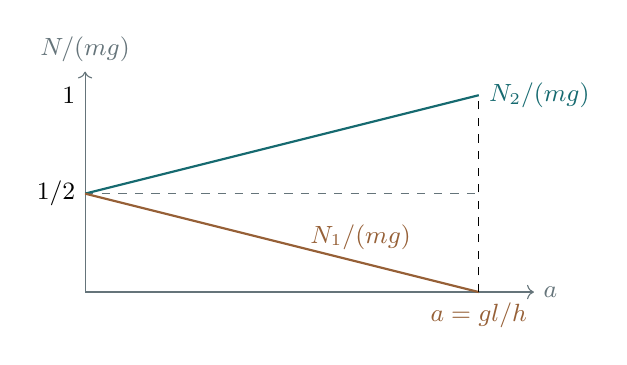
\begin{tikzpicture}[x=1cm,y=1cm]
\draw[->,color=muted] (0,0)--(5.7,0) node[right] {$a$};
\draw[->,color=muted] (0,0)--(0,2.8) node[above] {$N/(mg)$};
\draw[dashed,color=muted] (0,1.25)--(5,1.25);
\draw[thick,color=accent] (0,1.25)--(5,2.5) node[right] {$N_2/(mg)$};
\draw[thick,color=warm] (0,1.25)--(5,0) node[below] {$a=gl/h$};
\node[left] at (0,1.25) {$1/2$};\node[color=warm] at (3.5,.7) {$N_1/(mg)$};
\draw[dashed] (5,0)--(5,2.5);\node[left] at (0,2.5) {$1$};
\end{tikzpicture}
\figcaption{解图6.1B\quad 支持力随加速度作线性转移；右端是前轮刚离地的状态。}
\end{minipage}\end{center}
解图6.1B中两条斜线的和始终为1，说明竖直总支持力等于重力。后轮摩擦上限取上升载荷线对应的 $\mu N_2$，随加速度增加。

由后两式得 $N_2-N_1=mah/l$，与支持力之和联立：
\[
 N_1=\frac m2\left(g-\frac{ha}{l}\right),\qquad
 N_2=\frac m2\left(g+\frac{ha}{l}\right).
\]
后轮需要的驱动力为 $ma$，不滑动要求 $ma\le\mu N_2$，所以
\[\result{\mu\ge\frac{2la}{gl+ha}.}\]
这一结果以两轮都接地为前提，故还需 $a\le gl/h$（$h>0$）。当 $a=gl/h$ 时前轮支持力为零。再增大加速度，车身开始以前轮离地的姿态运动。负加速度使前轮增载、后轮减载；刹车时需按实际制动轮重新列摩擦条件。$h=0$ 时两轮各承担 $mg/2$，得到 $\mu\ge2a/g$。
\subsubsection*{路面给定时，先打滑还是先抬轮}
仍按解图6.1A的两轴接地模型，设$h>0$，把不打滑条件保持为未除式：
\[
(2l-\mu h)a\leq\mu gl,\qquad 0\leq a\leq\frac{gl}{h}.
\]
若$2l-\mu h>0$，才可直接除得摩擦给出的加速度上限
$a_f=\mu gl/(2l-\mu h)$。
比较$a_f$与解图6.1B前轮载荷降到零时的$a_w=gl/h$，有
\[
a_f\leq a_w\quad\Longleftrightarrow\quad\mu h\leq l.
\]
因此同时满足摩擦与接地的范围为
\[
0\leq a\leq a_{\max},\qquad
a_{\max}=\begin{cases}
\displaystyle\frac{\mu gl}{2l-\mu h},&0\leq\mu\leq l/h,\\[5pt]
\displaystyle\frac{gl}{h},&\mu\geq l/h.
\end{cases}
\]
在$\mu=l/h$时，两种临界状态同时到达：$N_1=0,N_2=mg$，
且$ma=\mu mg$。路面更粗糙时，前轮载荷首先降为零，两轮接地的平动过程在这里结束。
特别当$2l-\mu h\leq0$，摩擦不等式本身对非负$a$不再设上限，
此时两轮接地的加速度范围仍由 $a\leq gl/h$ 确定。

也可令$u=ah/(gl)$、$\kappa=\mu h/l$，
把两项条件化成$2u\leq\kappa(1+u)$与$0\leq u\leq1$。
两个无量纲条件在 $\kappa=1,u=1$ 处同时取等号。
当$h=0$时不使用含$1/h$的式子，而回到$N_1=N_2=mg/2$，
得到$a\leq\mu g/2$；此时加速度改变时，两个支持力始终各为 $mg/2$。


\Needspace{18\baselineskip}

\pdfbookmark[2]{第 2 题 均匀圆柱体绕斜向质心轴的转动惯量}{q2}

\section*{第 2 题\quad 均匀圆柱体绕斜向质心轴的转动惯量}

\tagline{M-06-02}

如图6.2,质量为\(m\)的均匀圆柱体,截面半径为\(R\),长为\(2R\).试求:圆柱体绕通过质心及两底面边缘的转轴(图6.2中的\(\sigma_{1}\)或\(\sigma_{2}\))的转动惯量.

\begin{center}\begin{minipage}{\linewidth}\centering
\begin{tikzpicture}[font=\small]
\draw[object](-1.5,-1.5)rectangle(1.5,1.5);
\draw[axis](-2.4,0)--(2.5,0)node[right]{$\sigma_3$};
\draw[axis](0,-2.15)--(0,2.15)node[above]{$\sigma_4$};
\draw[axis](-2,-2)--(2,2)node[above right]{$\sigma_1$};
\draw[axis](-2,2)--(2,-2)node[below right]{$\sigma_2$};
\fill(0,0)circle(1.7pt);\node at(.35,-.65){$O$};
\draw[<->](-1.5,-2.65)--(1.5,-2.65)node[midway,below]{$2R$};
\draw[<->](-2.55,0)--(-2.55,1.5)node[midway,left]{$R$};
\node at(0,-3.5){中轴所在截面；$\sigma_5$垂直图面};
\end{tikzpicture}
\figcaption{图 6.2\quad 长与直径相等；对角轴穿过质心及两底面边缘。}
\end{minipage}\end{center}

\Needspace{5\baselineskip}\subsection*{解答}

\begin{center}\begin{minipage}{\linewidth}\centering
\begin{tikzpicture}[font=\small]
\draw[object](-1.5,-1.5)rectangle(1.5,1.5);
\draw[axis](-2.4,0)--(2.5,0)node[right]{$\sigma_3$};
\draw[axis](0,-2.15)--(0,2.15)node[above]{$\sigma_4$};
\draw[axis](-2,-2)--(2,2)node[above right]{$\sigma_1$};
\draw[axis](-2,2)--(2,-2)node[below right]{$\sigma_2$};
\fill(0,0)circle(1.7pt);\node at(.35,-.65){$O$};
\draw[<->](-1.5,-2.65)--(1.5,-2.65)node[midway,below]{$2R$};
\draw[<->](-2.55,0)--(-2.55,1.5)node[midway,left]{$R$};
\node at(0,-3.5){中轴所在截面；$\sigma_5$垂直图面};
\end{tikzpicture}
\figcaption{解图 6.2A\quad 两组过同一原点的正交轴有相同惯量和。}
\end{minipage}\end{center}
圆柱长为 $2R$，故解图6.2A中的两条对角轴 $\sigma_1,\sigma_2$ 相互垂直，与中轴均成 $45^\circ$；$\sigma_5$ 垂直这个轴平面。先证明适用于三维物体的正交轴和关系。质元坐标为 $(x_i,y_i,z_i)$ 时，
\[
\begin{aligned}
 I_x&=\sum_i\Delta m_i(y_i^2+z_i^2),\\
 I_y&=\sum_i\Delta m_i(z_i^2+x_i^2),\\
 I_z&=\sum_i\Delta m_i(x_i^2+y_i^2).
\end{aligned}
\]
相加得到 $I_x+I_y+I_z=2\sum_i\Delta m_i r_i^2$。同一原点下，该和与正交轴组的朝向无关。因此
\[
 I_1+I_2+I_5=I_3+I_4+I_5,\qquad
 2I=I_3+I_4=\frac12mR^2+I_4.
\]
上式中的$I_1=I_2$还用了圆柱的镜面对称性：将圆柱关于横向中面反射，
解图6.2A的$\sigma_1,\sigma_2$互换，而质量分布不变。
也可从中轴、横向轴这两条主轴直接投影：
\[
I(\alpha)=I_3\cos^2\alpha+I_4\sin^2\alpha.
\]
混合惯量积分因镜面对称为零；本题$\alpha=45^\circ$，两项权重各为$1/2$，
所以才可把$I_1+I_2$写成$2I$。
本题的两条斜轴相互垂直，可以与 $\sigma_5$ 组成一组正交轴。若改变柱长，可直接用投影式分别求两条斜轴的惯量。

圆柱的三维轴和使用三个坐标的平方；圆片的垂直轴关系在下面单独用于每一薄片。

\begin{center}\begin{minipage}{\linewidth}\centering
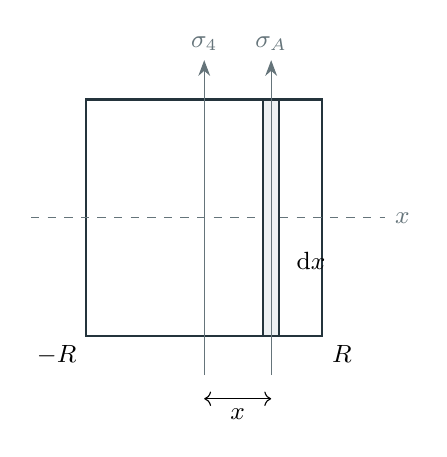
\begin{tikzpicture}[font=\small]
\draw[object](-1.5,-1.5)rectangle(1.5,1.5);
\draw[guide](-2.2,0)--(2.3,0)node[right]{$x$};
\draw[object,fill=rulegray!40](.75,-1.5)rectangle(.95,1.5);
\draw[axis](0,-2)--(0,2)node[above]{$\sigma_4$};
\draw[axis](.85,-2)--(.85,2)node[above]{$\sigma_A$};
\draw[<->](0,-2.3)--(.85,-2.3)node[midway,below]{$x$};
\node[right]at(1.05,-.55){$\dd x$};
\node[below left]at(-1.5,-1.5){$-R$};\node[below right]at(1.5,-1.5){$R$};
\end{tikzpicture}
\figcaption{解图 6.2B\quad 薄圆片先求直径轴惯量，再平移 $|x|$ 到圆柱横向质心轴。}
\end{minipage}\end{center}
解图6.2B在中轴坐标 $x$ 处切出厚度 $\dd x$ 的薄圆片，其质量 $\dd m=m\dd x/(2R)$。薄片轴向惯量为 $\dd I_C=\dd mR^2/2$；薄片的两条直径轴等价，且垂直轴定理给 $\dd I_C=2\dd I_A$，故
\[
 \dd I_A=\frac14R^2\dd m=\frac{mR}{8}\dd x.
\]
将薄片直径轴平移至整个圆柱的横向质心轴，距离为 $|x|$：
\[
 \dd I_4=\dd I_A+x^2\dd m
 =\frac{mR}{8}\dd x+\frac{m}{2R}x^2\dd x.
\]
积分并代回轴和关系：
\[
\begin{aligned}
 I_4&=\frac{mR}{8}\int_{-R}^{R}\dd x+
 \frac{m}{2R}\int_{-R}^{R}x^2\dd x
 =\frac14mR^2+\frac13mR^2=\frac7{12}mR^2,\\
 I&=\frac12\left(\frac12+\frac7{12}\right)mR^2
 =\result{\frac{13}{24}mR^2}.
\end{aligned}
\]
从主惯量投影看，轴向主惯量为 $mR^2/2$，横向为 $7mR^2/12$，斜轴惯量是二者按 $\cos^245^\circ$、$\sin^245^\circ$ 加权之和。
\subsubsection*{三维轴和与薄圆片的径向积分}
三维轴和关系中，$r_i^2=x_i^2+y_i^2+z_i^2$ 是质元到公共原点 $O$ 的距离平方。每条转轴的惯量由垂直于该轴的两个坐标平方组成，将三个定义式逐项相加，得到
\[
\begin{aligned}
I_x+I_y+I_z
&=\sum_i\Delta m_i[(y_i^2+z_i^2)+(z_i^2+x_i^2)+(x_i^2+y_i^2)]\\
&=2\sum_i\Delta m_i(x_i^2+y_i^2+z_i^2)
=2\sum_i\Delta m_i r_i^2.
\end{aligned}
\]
转动坐标轴不改变$r_i$，故对解图6.2A的两组轴分别有
\[
I_1+I_2=2\sum_i\Delta m_i r_i^2-I_5,
\qquad
I_3+I_4=2\sum_i\Delta m_i r_i^2-I_5.
\]
两边相减才得到$I_1+I_2=I_3+I_4$。
各轴通过同一点、每组三轴两两正交时，这一证明对三维物体和薄片、均匀与非均匀质量分布都成立。

薄圆片的垂直轴定理则用在解图6.2C所示的局部圆面上。
该片内两条直径轴为$\sigma_A,\sigma_B$，
面法线轴为$\sigma_C$；忽略$\dd x$厚度的高阶效应，
质元到面法线的距离平方恰为到两条面内轴的距离平方之和，因而
\[
\dd I_C=\dd I_A+\dd I_B,
\qquad \dd I_A=\dd I_B.
\]
\begin{center}\begin{minipage}{\linewidth}\centering
\begin{tikzpicture}
\draw[object](0,0)circle(1.3);
\draw[axis](-1.8,0)--(1.9,0)node[right]{$\sigma_B$};
\draw[axis](0,-1.8)--(0,1.9)node[above]{$\sigma_A$};
\node[fill=white,inner sep=1pt]at(0,0){$\odot$};
\node[above left]at(-.12,.12){$O_A$};
\fill(.8,.45)circle(1.6pt)node[above right]{$\delta m$};
\draw[guide](.8,0)--(.8,.45)--(0,.45);
\draw[<->](0,0)--(-.919238816,-.919238816)node[midway,below left]{$R$};
\node[align=left,anchor=west]at(2.8,.7){$\sigma_C$垂直圆面\\$\dd I_C=\dd I_A+\dd I_B$\\两条直径轴因对称而等价};
\end{tikzpicture}
\figcaption{解图6.2C\quad 薄圆片的三条局部轴；圆面上的$\delta m$用于解释垂直轴关系。}
\end{minipage}\end{center}
圆片的面密度为$\dd m/(\pi R^2)$。
把圆片再分成半径$s$、宽$\dd s$的圆环，
圆环质量为$2\dd m\,s\dd s/R^2$，所以
\[
\dd I_C=\int_0^R s^2\frac{2\dd m}{R^2}s\dd s
=\frac12R^2\dd m.
\]
由解图6.2B中均匀圆柱的轴向质量分配$\dd m=m\dd x/(2R)$，
逐步代入可得
\[
\dd I_C=\frac12\frac{m}{2R}\dd x\,R^2
=\frac{mR}{4}\dd x,
\qquad
\dd I_A=\frac12\dd I_C=\frac{mR}{8}\dd x.
\]
薄片绕自身直径轴已有惯量 $\dd I_A$，平移后再加 $x^2\dd m$，两项共同组成薄片对 $\sigma_4$ 的惯量。
两项积分的边界和数值分别是
\[
\begin{aligned}
\int_{-R}^{R}\frac{mR}{8}\dd x
&=\frac{mR}{8}[x]_{-R}^{R}=\frac14mR^2,\\
\int_{-R}^{R}\frac{m}{2R}x^2\dd x
&=\frac{m}{2R}\left[\frac{x^3}{3}\right]_{-R}^{R}
=\frac13mR^2.
\end{aligned}
\]
于是$I_4=7mR^2/12$，再由$2I=mR^2/2+I_4$还原
\[
I=\frac14mR^2+\frac12I_4
=\left(\frac14+\frac7{24}\right)mR^2
=\frac{13}{24}mR^2.
\]
所求值介于中轴惯量$12mR^2/24$与横轴惯量$14mR^2/24$之间，
符合$45^\circ$主轴投影的等权结果。
解图6.2A、B的轴向截面均按边长$2R$的正方形绘制，
薄片坐标$x$与轴间平移距离$|x|$在同一几何比例下对应。


\Needspace{18\baselineskip}

\pdfbookmark[2]{第 3 题 桌边细杆开始滑动的临界角}{q3}

\section*{第 3 题\quad 桌边细杆开始滑动的临界角}

\tagline{M-06-03}

如图,长为\(l\)的均匀细杆水平地放置在桌面上,质心离桌边缘的距离为\(b\),从静止下落.

已知杆与桌边缘之间的摩擦系数为 \(\mu\). 试求杆开始滑动时 的角度
\(\theta_{C}\).

\begin{center}\begin{minipage}{\linewidth}\centering
\begin{tikzpicture}[font=\small]
\draw[object](-2,0)--(0,0)--(0,-2);\draw[object,line width=2pt](-1.3,0)--(3.5,0);\fill(0,0)circle(2pt)node[below left]{$A$};\fill(1.1,0)circle(2pt)node[above]{$C$};\draw[<->](0,.6)--(1.1,.6)node[midway,above]{$b$};\node[below]at(2.8,-.2){杆长 $l$};
\end{tikzpicture}
\figcaption{图 6.3\quad 质心在桌边外侧；初态水平静止。}
\end{minipage}\end{center}

\Needspace{5\baselineskip}\subsection*{解答}

\begin{center}\begin{minipage}{\linewidth}\centering
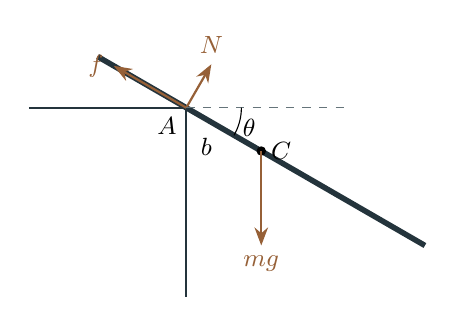
\begin{tikzpicture}[font=\small]
\draw[object](-2,0)--(0,0)--(0,-2.4);
\draw[object,line width=2pt](-1.125833025,.65)--(3.031088913,-1.75);
\coordinate(C)at(.952627944,-.55);
\node[below left]at(0,0){$A$};\fill(C)circle(1.7pt)node[right]{$C$};
\draw[force](0,0)--(-.921362490,.531948882)node[left]{$f$};
\draw[force](0,0)--(.318741618,.552076677)node[above]{$N$};
\draw[force](C)--++(0,-1.2)node[below]{$mg$};
\draw[guide](0,0)--(2,0);\draw(.7,0)arc(0:-30:.7);
\node at(.8,-.25){$\theta$};\node[below left]at(.45,-.26){$b$};
\end{tikzpicture}
\figcaption{解图 6.3A\quad 桌角摩擦沿杆，支持力垂直杆；质心同时有切向和向心加速度。}
\end{minipage}\end{center}
杆的质心 $C$ 在桌边 $A$ 外侧，$AC=b>0$。解图6.3A取转下角 $\theta$ 为正，摩擦 $f$ 沿杆指向 $A$，支持力 $N$ 垂直杆；不滑动时 $A$ 固定。令
\[
 I_C=\frac1{12}ml^2,\quad I_A=I_C+mb^2,\quad \beta=\dot\omega.
\]
绕 $A$ 的重力矩给 $I_A\beta=mgb\cos\theta$。质心法向、切向方程为
\[
 f-mg\sin\theta=mb\omega^2,\qquad
 mg\cos\theta-N=mb\beta.
\]
这里“法向”指向质心圆周轨迹的圆心$A$，沿杆指回桌角；“切向”则垂直杆。重力沿杆向外的投影为$mg\sin\theta$，摩擦一部分抵消这一分量，另一部分提供 $mb\omega^2$ 的向心需求。垂杆方向上，重力的一部分用于产生$mb\beta$，剩余部分才是支持力$N$。两种分量分别进入沿杆与垂杆方程，接触力须由动力学计算。

因此 $N=mg\cos\theta(1-mb^2/I_A)=mgI_C\cos\theta/I_A$。为求 $f$，用
\[
 \dot\omega=\omega\frac{\dd\omega}{\dd\theta}
 =\frac{mgb}{I_A}\cos\theta.
\]
从 $(\theta,\omega)=(0,0)$ 积分，
\[
 \int_0^\omega\omega\dd\omega
 =\frac{mgb}{I_A}\int_0^\theta\cos\theta\dd\theta,
 \qquad \omega^2=\frac{2mgb}{I_A}\sin\theta.
\]
同一结果也由 $mgb\sin\theta=I_A\omega^2/2$ 得到。代入法向方程，
\[
 f=mg\sin\theta\left(1+\frac{2mb^2}{I_A}\right)
 =mg\frac{I_C+3mb^2}{I_A}\sin\theta.
\]
将两个接触力相除可把判断写得更直接：
\[\frac fN=\frac{I_C+3mb^2}{I_C}\tan\theta
=\left(1+\frac{36b^2}{l^2}\right)\tan\theta.\]
从水平静止释放后，$0\le\theta<\pi/2$内这个比值从零严格增加，故与$\mu$的第一次相等就是首次滑动，不会在此前已有别的临界角。与此同时$N$仍为正，因此这里先失去的是不滑动约束。

达到 $f=\mu N$ 时开始滑动：
\[
 (I_C+3mb^2)\sin\theta_C=\mu I_C\cos\theta_C,
 \qquad\result{\tan\theta_C=\frac{\mu l^2}{l^2+36b^2}.}
\]
有限 $\mu$ 给 $0\le\theta_C<\pi/2$，临界时 $N>0$；$\mu=0$ 时刚偏转即滑动。当 $b=0$ 时，重力对桌角的力矩为零，水平静止的杆保持平衡；题设由重力启动的过程取 $b>0$。
\subsubsection*{质心加速度、桌角支持力与起滑条件}
解图6.3B把质心轨道另画为圆弧。
令$\vect e_r$从$A$指向$C$，$\vect e_\theta$沿转下方向，
不滑动阶段的质心加速度为
\[
\vect a_C=-b\omega^2\vect e_r+b\beta\vect e_\theta.
\]
图中的$a_n$指向$A$，$a_\tau$垂直$AC$且朝转下方向。
桌角支持力垂直于杆，沿质心圆轨迹的切线方向。质心的向心加速度沿杆指向桌角，所以两个分量方程分别沿杆和垂直杆写。
\begin{center}\begin{minipage}{\linewidth}\centering
\begin{tikzpicture}
\coordinate(A)at(0,0);\coordinate(C)at(1.732050808,-1);
\draw[guide](2,0)arc(0:-58:2);\draw[object](A)--(C);
\fill(A)circle(1.6pt)node[above left]{$A$};
\fill(C)circle(1.6pt)node[above right]{$C$};
\draw[motion](C)--(.866025404,-.5)node[above left]{$a_n=b\omega^2$};
\draw[motion](C)--(1.299038106,-1.75)node[below]{$a_\tau=b\beta$};
\node at(.72,-.12){$b$};
\draw[guide](A)--(2.3,0);\draw(.5,0)arc(0:-30:.5);
\node at(.85,-.25){$\theta$};
\node[align=left,anchor=west]at(3,-.6){$\vect e_r$沿$A\to C$\\$\vect e_\theta$沿转下方向};
\end{tikzpicture}
\figcaption{解图6.3B\quad 向心与切向加速度分别列入两个投影方程；示例倾角为$30^\circ$。}
\end{minipage}\end{center}
由重力矩先得
\[
\beta=\frac{mgb}{I_C+mb^2}\cos\theta,
\qquad
mb\beta=\frac{mb^2}{I_C+mb^2}mg\cos\theta.
\]
于是支持力的每一步消元为
\[
N=mg\cos\theta-mb\beta
=\left(1-\frac{mb^2}{I_C+mb^2}\right)mg\cos\theta
=\frac{I_C}{I_C+mb^2}mg\cos\theta.
\]
求角速度时也可先保留积分常量$C_0$：
\[
\omega\dd\omega=\frac{mgb}{I_C+mb^2}\cos\theta\dd\theta,
\qquad
\frac12\omega^2=\frac{mgb}{I_C+mb^2}\sin\theta+C_0.
\]
水平静止初值同时给出$\theta=0,\omega=0$，故$C_0=0$。
正弦的自变量是倾角$\theta$，角加速度$\beta$只通过转动方程进入积分。
代回沿杆方程就恢复前面$f$的两个贡献：抵消重力沿杆分量，另提供向心加速度。

对跨在桌边的均匀杆通常有$0<b<l/2$；$b=l/2$可作为桌角恰在端点的极限。
在$0<\theta<\pi/2$中，
\[
\frac{\dd}{\dd\theta}\left(\frac fN\right)
=\frac{I_C+3mb^2}{I_C}\sec^2\theta>0.
\]
正导数表明所需摩擦比随倾角增大，从零逐渐升到静摩擦上限。
有限$\mu$的交点处$\cos\theta_C>0$，所以桌角仍对杆施加正的支持力。当 $0<b<l/2$，杆超过这个倾角后，沿杆向外的滑动使接触位置逐渐移向杆的内端。当 $b=l/2$，桌角起初就在内端，滑动一开始，杆即离开桌角。


\Needspace{18\baselineskip}

\pdfbookmark[2]{第 4 题 实心圆柱体绕桌边下滚与开始滑动}{q4}

\section*{第 4 题\quad 实心圆柱体绕桌边下滚与开始滑动}

\tagline{M-06-04}

如图6.4,实心圆柱体从桌边由静止下滚,圆柱体与桌边之间的摩擦系数为\(\mu\).圆

柱体下滚过程中所转过的角度用 \(\theta\) 表示(如图6.4
所示).试求圆柱体开始相对桌边滑动时相应角度 \(\theta\)
所满足的关系式,并用图解法在图上标出这个角度以及不滑动的转角范围.

初态从静止作无穷小偏离后开始运动。

\begin{center}\begin{minipage}{\linewidth}\centering
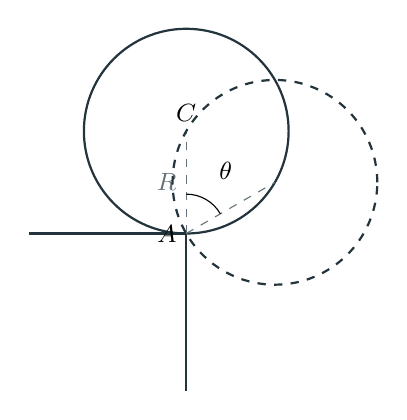
\begin{tikzpicture}[font=\small]
\draw[object](-2,0)--(0,0)--(0,-2);\draw[object](0,1.3)circle(1.3);\draw[guide](0,0)--(0,1.3)node[midway,left]{$R$};\node[left]at(0,0){$A$};\node[above]at(0,1.3){$C$};\draw[guide](0,0)--(1.125833025,.65);\draw[object,dashed](1.125833025,.65)circle(1.3);\draw(0,.5)arc(90:30:.5);\node at(.5,.8){$\theta$};
\end{tikzpicture}
\figcaption{图 6.4\quad 圆心绕固定桌角向右下方移动。}
\end{minipage}\end{center}

\Needspace{5\baselineskip}\subsection*{解答}

\begin{center}\begin{minipage}{\linewidth}\centering
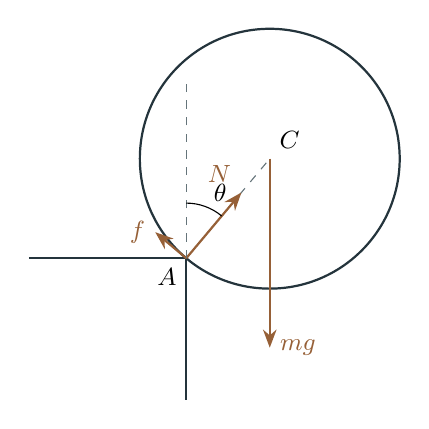
\begin{tikzpicture}[font=\small]
\draw[object](-2,0)--(0,0)--(0,-1.8);
\coordinate(C)at(1.060599556,1.263973331);\draw[object](C)circle(1.65);
\draw[guide](0,0)--(C);
\draw[force](0,0)--(.700541357,.834872679)node[above left]{$N$};
\draw[force](0,0)--(-.393923101,.330540729)node[left]{$f$};
\draw[force](C)--++(0,-2.4)node[right]{$mg$};
\draw[guide](0,0)--(0,2.3);\draw(0,.7)arc(90:50:.7);
\node at(.43,.83){$\theta$};\node[above right]at(C){$C$};
\node[below left]at(0,0){$A$};
\end{tikzpicture}
\figcaption{解图 6.4A\quad 支持力沿桌角至圆心，摩擦沿接触切线；角度从竖直向上量起。}
\end{minipage}\end{center}
解图6.4A中 $\theta$ 是 $AC$ 相对初始竖直方向的转角。不滑动阶段圆柱绕桌角 $A$ 转动，$I_A=I_C+mR^2=3mR^2/2$。径向、切向及绕 $A$ 的方程为
\[
 mg\cos\theta-N=mR\dot\theta^2,\quad
 mg\sin\theta-f=mR\ddot\theta,\quad
 mgR\sin\theta=I_A\ddot\theta.
\]
故 $\ddot\theta=2g\sin\theta/(3R)$、$f=mg\sin\theta/3$。利用 $\ddot\theta=\dot\theta\,\dd\dot\theta/\dd\theta$，积分得到
\[
 \frac12\dot\theta^2=-\frac{2g}{3R}\cos\theta+C_0,
 \quad C_0=\frac{2g}{3R},\quad
 \dot\theta^2=\frac{4g}{3R}(1-\cos\theta).
\]
能量法保留同样的初态与约束：$mgR(1-\cos\theta)=I_A\dot\theta^2/2$，也给出上式。代回径向方程：
\[
 N=mg\left[\cos\theta-\frac43(1-\cos\theta)\right]
 =\frac{mg}{3}(7\cos\theta-4).
\]
不滑动要求 $N\ge0$ 且 $f\le\mu N$，临界角满足
\[\result{\sin\theta_C=\mu(7\cos\theta_C-4).}\]
\begin{center}\begin{minipage}{\linewidth}\centering
\begin{tikzpicture}[font=\small,x=4.4cm,y=2.8cm]
\fill[accent!7](0,0)rectangle(.584295501,1.05);
\draw[axis](0,0)--(1.1,0)node[right]{$\theta/\mathrm{rad}$};
\draw[axis](0,0)--(0,1.25)node[above]{$y$};
\draw[traj,domain=0:.584295501,samples=70]plot(\x,{sin(deg(\x))});
\draw[thick,color=warm,domain=0:.584295501,samples=70]plot(\x,{.3*(7*cos(deg(\x))-4)});
\draw[traj,dashed,domain=.584295501:.962550748,samples=60]plot(\x,{sin(deg(\x))});
\draw[thick,color=warm,dashed,domain=.584295501:.962550748,samples=60]plot(\x,{.3*(7*cos(deg(\x))-4)});
\draw[guide](.584295501,0)--(.584295501,.551611896);
\fill(.584295501,.551611896)circle(.8pt);
\node[below]at(.584295501,0){$\theta_C$};
\node[below]at(.962550748,0){$\theta_0$};
\node[left]at(0,.9){$3\mu$};
\node[above]at(.8,.85){$\sin\theta$};
\draw[guide](.25,.834716)--(.36,1.06);
\node[above]at(.39,1.06){$\mu(7\cos\theta-4)$};
\draw[line width=2pt,accent](0,-.27)--(.584295501,-.27)node[midway,below]{不滑};
\end{tikzpicture}
\figcaption{解图 6.4B\quad 取$\mu=0.3$，交点与零点按计算定位；交点后的虚线只延拓纯滚表达式。}
\end{minipage}\end{center}
解图6.4B画的是无量纲的 $3f/(mg)=\sin\theta$ 与 $3\mu N/(mg)=\mu(7\cos\theta-4)$，交点给 $\theta_C$。前者递增，后者递减，在 $0\le\theta\le\arccos(4/7)$ 内只有一交点。不滑范围为 $0\le\theta\le\theta_C$。

若要在解图6.4B中准确定位交点，可令$z=\tan(\theta_C/2)$。
临界方程变为
\[
2z=\mu(3-11z^2),\qquad
z=\frac{\sqrt{1+33\mu^2}-1}{11\mu}
=\frac{3\mu}{1+\sqrt{1+33\mu^2}},
\]
\[
\theta_C=2\arctan\frac{3\mu}{1+\sqrt{1+33\mu^2}}\quad(\mu>0).
\]
只取正根；另一根对应负角，不属于由顶端向右下滚的过程。
图示$\mu=0.3$时，$\theta_C$约为$33.5^\circ$。
小$\mu$时$\theta_C\simeq3\mu$（弧度）；$\mu$增大时它趋近
$\arccos(4/7)$但始终小于该角，和图中滑动先于纯滚延拓的零压力点相符。

对有限正 $\mu$，$7\cos\theta_C-4=\sin\theta_C/\mu>0$，因此滑动先于脱离。图中 $\theta_0=\arccos(4/7)$ 是纯滚表达式的零支持力角。实际圆柱先在 $\theta_C$ 滑动，随后由滑动方程求支持力降到零的位置。严格位于顶端且完全静止是非稳定平衡，本题下滚理解为无穷小扰动后的过程。
\subsubsection*{积分步骤与曲线有效区间}
由转动方程消去$I_A$得到$\ddot\theta=2g\sin\theta/(3R)$。
这里对角速度使用链式法则，导数的分母应为角度：
\[
\ddot\theta=\frac{\dd\dot\theta}{\dd t}
=\frac{\dd\dot\theta}{\dd\theta}\frac{\dd\theta}{\dd t}
=\dot\theta\frac{\dd\dot\theta}{\dd\theta}.
\]
所以积分的两端可直接写为
\[
\int_0^{\dot\theta}u\dd u
=\frac{2g}{3R}\int_0^\theta\sin v\dd v
=\frac{2g}{3R}(1-\cos\theta).
\]
若用不定积分，初值$\theta=0,\dot\theta=0$给
$0=-2g/(3R)+C_0$，即$C_0=2g/(3R)$。
无滑接触点$A$的速度为零，支持力和静摩擦均不对圆柱做功；
因此能量式中的动能既可写成$I_A\dot\theta^2/2$，
也可分成质心平动与自转两项：
\[
\frac12mR^2\dot\theta^2+\frac12I_C\dot\theta^2
=\frac34mR^2\dot\theta^2.
\]
两种写法都包含质心平动与圆柱自转，纯滚时它们的速度通过同一个角速度联系起来。

解图6.4B的上升曲线表示所需摩擦，下弯曲线表示可供上限，
纵坐标分别乘同一个$3/(mg)$，才可以直接比较。
在压力为正的纯滚区间中，令$q= f/N$，有
\[
q(\theta)=\frac{\sin\theta}{7\cos\theta-4},
\qquad
q'(\theta)=\frac{7-4\cos\theta}{(7\cos\theta-4)^2}>0.
\]
从顶点的$q=0$到$\theta_0=\arccos(4/7)$前的$q\to+\infty$，
任何有限正$\mu$都只有一个交点。
因此实线区间$0\leq\theta\leq\theta_C$满足无滑条件；
交点之后的虚线延续纯滚表达式，实际受力从交点起按动摩擦和独立的自转速度计算。
图示$\mu=0.3$时，计算给
\[
\theta_C=0.5842955010\,\mathrm{rad}=33.4776662^\circ,
\qquad
\theta_0=0.9625507479\,\mathrm{rad}=55.1500954^\circ.
\]
在临界处$N_C=mg\sin\theta_C/(3\mu)>0$，
所以应先换成滑动方程；“先滑动”与“已经离边”对应不同的接触状态。
当$\mu\to0^+$时临界角趋零；当$\mu\to\infty$时，
$\theta_0-\theta_C\sim1/(7\mu)$，
有限摩擦的交点始终在零压力延拓角之前。

严格位于最高点并完全静止时，重力矩为零，数学解会一直停在顶点。
可先从一个任意小的正角$\theta_i$静止释放，得到
\[
\dot\theta^2=\frac{4g}{3R}(\cos\theta_i-\cos\theta),
\qquad
N=\frac{mg}{3}(7\cos\theta-4\cos\theta_i),
\]
再取$\theta_i\to0^+$恢复本题关系。
这个有限初角模型也须先满足$\tan\theta_i\leq3\mu$，
若这一条件不满足，释放瞬间即开始滑动。


\Needspace{18\baselineskip}

\pdfbookmark[2]{第 5 题 甲虫落到可转动麦杆后的运动}{q5}

\section*{第 5 题\quad 甲虫落到可转动麦杆后的运动}

\tagline{M-06-05}

如图,均匀细麦杆长\(l\),可绕通过中心\(O\)的固定水平轴在铅垂面内自由转动.开始时麦杆静止于水平位置.一质量与麦杆相同的甲虫以速度\(v_{0}\)垂直落到麦杆的\(\frac{1}{4}\)长度处,落下后立即向端点爬行.

试问:1. 为使麦杆以均匀的角速度转动,甲虫沿麦杆爬行的速度应是多少? 2.
甲虫轨迹的参变方程是什么? 3.
为了使甲虫在麦杆转到铅直位置前能爬到端点,甲虫下落速度 \(v_{0}\)
的最高值是多少?

\begin{center}\begin{minipage}{\linewidth}\centering
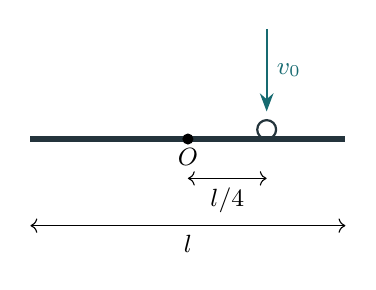
\begin{tikzpicture}[font=\small]
\draw[object,line width=2pt](-2,0)--(2,0);\fill(0,0)circle(2pt)node[below]{$O$};\draw[object](1,.12)circle(.12);\draw[motion](1,1.4)--(1,.35)node[midway,right]{$v_0$};\draw[<->](0,-.5)--(1,-.5)node[midway,below]{$l/4$};\draw[<->](-2,-1.1)--(2,-1.1)node[midway,below]{$l$};
\end{tikzpicture}
\figcaption{图 6.5\quad 甲虫落点离中心 $l/4$，随后沿杆向右端爬行。}
\end{minipage}\end{center}

\Needspace{5\baselineskip}\subsection*{解答}

\begin{center}\begin{minipage}{\linewidth}\centering
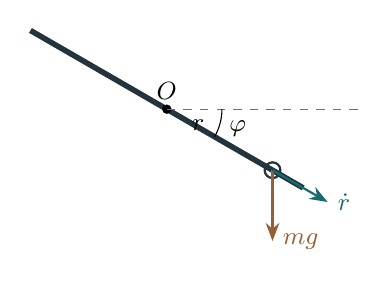
\begin{tikzpicture}[font=\small]
\draw[object,line width=2pt](-1.732050808,1)--(1.732050808,-1);
\fill(0,0)circle(1.7pt)node[above]{$O$};\coordinate(P)at(1.342339376,-.775);
\draw[object](P)circle(.1);\draw[force](P)--++(0,-.9)node[right]{$mg$};
\draw[motion](P)--++(.7,-.404145188)node[right]{$\dot r$};
\draw[guide](0,0)--(2.5,0);\draw(.7,0)arc(0:-30:.7);
\node at(.9,-.25){$\varphi$};\node[above left]at(.6,-.4){$r$};
\end{tikzpicture}
\figcaption{解图 6.5A\quad $r$ 为甲虫到支轴距离，$\dot r$ 为相对杆的径向爬速。}
\end{minipage}\end{center}
甲虫落点到杆中心的距离 $r_0=l/4$；杆与甲虫的质量均为 $m$。碰撞期间支轴冲量关于 $O$ 的矩为零，重力冲量矩可忽略。系统关于 $O$ 的角动量守恒：
\[
 mv_0\frac l4=\left(\frac1{12}ml^2+m\frac{l^2}{16}\right)\omega,
 \qquad\result{\omega=\frac{12v_0}{7l}.}
\]
碰后麦杆自身的重力通过 $O$，只有甲虫产生重力矩。解图6.5A以向下转角 $\varphi=\omega t$ 为正，$I(t)=ml^2/12+mr^2$。恒角速度要求
\[
 mgr\cos\varphi=\frac{\dd(I\omega)}{\dd t}
 =\omega(2mr\dot r),
 \qquad\result{\dot r=\frac g{2\omega}\cos(\omega t).}
\]
这是相对杆的爬行速度；甲虫在空间的速度还含切向分量 $r\omega$。积分时先保留上下限和初始位置：
\[
 \int_{l/4}^{r(t)}\dd r=\frac g{2\omega}\int_0^t\cos(\omega t')\dd t'
 =\frac g{2\omega^2}\sin(\omega t).
\]
积分起点取落点半径 $r(0)=l/4$，于是
\[
 r(t)=\frac l4+\frac g{2\omega^2}\sin(\omega t),\qquad
 \varphi(t)=\omega t.
\]
\Needspace{19\baselineskip}
\begin{center}\begin{minipage}{\linewidth}\centering
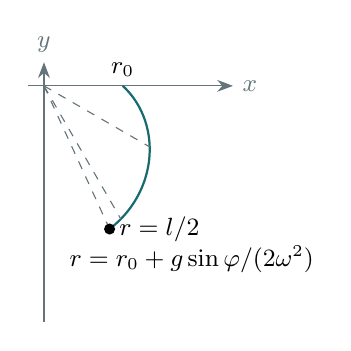
\begin{tikzpicture}[font=\small]
\draw[axis](-.2,0)--(2.4,0)node[right]{$x$};\draw[axis](0,-3)--(0,.3)node[above]{$y$};\draw[traj,domain=0:65.380022671,samples=70]plot({(1+1.1*sin(\x))*cos(\x)},{-(1+1.1*sin(\x))*sin(\x)});\foreach \t in {0,30,60,65.380022671}{\draw[guide](0,0)--({(1+1.1*sin(\t))*cos(\t)},{-(1+1.1*sin(\t))*sin(\t)});}\node[above]at(1,0){$r_0$};\fill(.833195581,-1.818181818)circle(2pt)node[right]{$r=l/2$};\node[right]at(.2,-2.2){$r=r_0+g\sin\varphi/(2\omega^2)$};
\end{tikzpicture}
\figcaption{解图 6.5B\quad 甲虫空间轨迹为极径随转角增长的曲线；在到端时截断。}
\end{minipage}\end{center}
解图6.5B按 $x=r\cos\varphi$、$y=-r\sin\varphi$ 将极坐标轨迹转成直角坐标。图中甲虫在杆转到铅直前到端，所以曲线在 $r=l/2$ 处结束。如果转到铅直仍未到端，匀速向外爬行这一段止于 $\varphi=\pi/2$，此时 $\dot r=0$。

杆转到铅直时 $t_v=\pi/(2\omega)$。甲虫要在此前或同时到端，需
\[
 \frac l4+\frac g{2\omega^2}\ge\frac l2
 \Longrightarrow \omega^2\le\frac{2g}{l}
 \Longrightarrow\result{v_0\le\frac7{\sqrt{72}}\sqrt{gl}.}
\]
若“之前”取严格含义，则改为严格小于；等号意味着恰在铅直时到端。到端后若甲虫留在杆端，惯量固定，随后的角速度由重力矩决定。
\subsubsection*{角动量变化、积分常量与到端时刻}
落杆瞬间的惯量可分项算清：
\[
I_0=\left(\frac1{12}+\frac1{16}\right)ml^2
=\frac7{48}ml^2,
\qquad
\omega=\frac{mv_0l/4}{7ml^2/48}=\frac{12v_0}{7l}.
\]
径向爬速不贡献关于$O$的角动量，因为径向速度与矢径平行。
但它会改变$r$及转动惯量；碰后系统的外力矩为$mgr\cos\varphi$，并不为零。
完整角动量方程展开为
\[
mgr\cos\varphi
=\left(\frac1{12}ml^2+mr^2\right)\dot\omega
+2mr\dot r\,\omega.
\]
只有代入题设$\dot\omega=0$以后，才得到所需爬速。
其中$r>0,\omega>0$；从$\varphi=0$转到$\pi/2$的过程中，
$\cos\varphi\geq0$，所以甲虫始终向外爬，爬速逐渐减小。
若甲虫不爬，第二项消失，重力矩便使角速度增大。

积分也可写成$r=g\sin(\omega t)/(2\omega^2)+C_0$。
将$t=0,r=l/4$同时代入得$C_0=l/4$，
再与$\varphi=\omega t$组成极坐标参变方程。
解图6.5B的坐标约定是右方为$x$正向、上方为$y$正向，
而$\varphi$向下为正，故
\[
x(t)=\left[\frac l4+\frac g{2\omega^2}\sin(\omega t)\right]\cos(\omega t),
\]
\[
y(t)=-\left[\frac l4+\frac g{2\omega^2}\sin(\omega t)\right]\sin(\omega t).
\]
这里$\dot r$与$r\omega$互相垂直，空间速率由这两个正交分量合成，为 $v=\sqrt{\dot r^2+r^2\omega^2}$。

到端条件可进一步求成时刻，令$\zeta=\omega^2l/(2g)$。
由$r(t_e)=l/2$得到
\[
\sin\varphi_e=\zeta,
\qquad \varphi_e=\arcsin\zeta,
\qquad t_e=\frac{\arcsin\zeta}{\omega}.
\]
因此 $0<\zeta\leq1$ 才会在 $0<\varphi\leq\pi/2$ 到端。当 $\zeta>1$，铅直时 $r=l/4+g/(2\omega^2)<l/2$，继续保持同一角速度将要求 $\dot r<0$。
$t_e\leq\pi/(2\omega)$恰与前面的$\omega^2\leq2g/l$相同。
等号给$\varphi_e=\pi/2$，严格小于给提前到端。
若“前”严格排除同时到达，$7\sqrt{gl/72}$是允许速度的上确界，
允许速度严格小于这个上确界。

解图6.5A、B采用同一示例$g/(2\omega^2)=1.1r_0$。
图中取$r_0$为长度单位，则$l/2=2$，
$30^\circ$时$r=1.55$，到端角为$\arcsin(1/1.1)=65.3800227^\circ$，
终点坐标为$(0.8331956,-1.8181818)$。
曲线和终点均由这些参数计算，到端时曲线截断。

\subsubsection*{碰撞与主动爬行的能量条件}
若先看甲虫被麦杆接住、尚未建立径向爬速的瞬间，
碰后的转动动能与碰前动能之比为
\[
\frac{K_+}{K_-}
=\frac{(mv_0r_0)^2/(2I_0)}{mv_0^2/2}
=\frac{mr_0^2}{I_0}=\frac37.
\]
这个捕获过程损失了碰前动能的$4/7$。
规定的爬行函数在$t=0^+$却要求$\dot r=g/(2\omega)$，
建立这部分径向速度需要甲虫主动作用；它不改变上述轴角动量，
建立径向速度所需的能量由甲虫的主动爬行动作提供。爬行阶段的运动由外重力矩与变化中的惯量联系起来。

若严格提前到端，甲虫停在$r=l/2$以后，
在 $\varphi<\pi/2$ 时外重力矩仍为正，惯量已经固定，角速度随之增加。
因此匀角速度公式与解图6.5B的轨迹均止于到端时刻；
恰在铅直时到端的情形可让这段匀速过程一直延续到铅直位置。


\Needspace{18\baselineskip}

\pdfbookmark[2]{第 6 题 圆柱滚上台阶的速度范围}{q6}

\section*{第 6 题\quad 圆柱滚上台阶的速度范围}

\tagline{M-06-06}

如图6.6,半径为\(R\)的均匀实心圆柱体在水平地面上作纯滚动,其中心\(C\)点的速

度为 \(v_{0}\), 它向前滚动时遇到一个高为 \(h\) 的台阶,
并发出完全非弹性碰撞. 设圆柱和台阶前缘之间的摩擦系数足够大.

试问：1.\(v_{0}\) 为何值时圆柱体能不脱离 A 点而滚上台阶继续前进？2.
对台阶高度 h 有什么限制？

\begin{center}\begin{minipage}{\linewidth}\centering
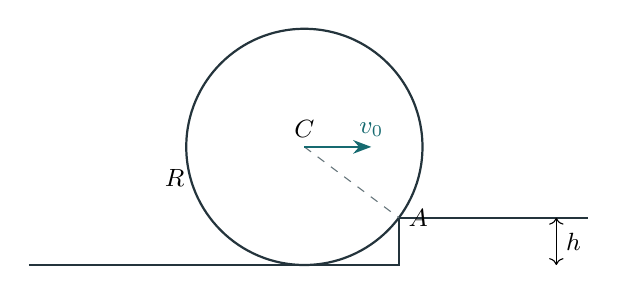
\begin{tikzpicture}[font=\small]
\draw[object](-3.7,0)--(1,0)--(1,.6)--(3.4,.6);\coordinate(A)at(1,.6);\coordinate(C)at(-.2,1.5);\draw[object](C)circle(1.5);\draw[guide](C)--(A);\node[above]at(C){$C$};\node[right]at(A){$A$};\draw[motion](C)--++(.85,0)node[above]{$v_0$};\draw[<->](3,0)--(3,.6)node[midway,right]{$h$};\node[left]at(-1.6,1.1){$R$};
\end{tikzpicture}
\figcaption{图 6.6\quad 碰前仍接地，台阶前缘 $A$ 是碰后上翻的接触点。}
\end{minipage}\end{center}

\Needspace{5\baselineskip}\subsection*{解答}

\begin{center}\begin{minipage}{\linewidth}\centering
\begin{tikzpicture}[font=\small]
\draw[object](-3,0)--(0,0)--(0,.6)--(3.3,.6);
\coordinate(A)at(0,.6);\coordinate(C)at(-1.2,1.5);
\draw[object](C)circle(1.5);\draw[object,dashed](0,2.1)circle(1.5);
\draw[guide](A)--(C);\draw[guide](A)--(0,2.1);
\node[right]at(A){$A$};\node[above left]at(C){$C$};
\node[right]at(.1,2.2){过顶};\node[above]at(-.6,1.05){$R$};
\draw[<->](2.7,0)--(2.7,.6)node[midway,right]{$h$};
\end{tikzpicture}
\figcaption{解图 6.6A\quad 圆心从碰后位置升到过顶位置，接触上翻须同时满足能量与压力条件。}
\end{minipage}\end{center}
先处理撞角，再处理绕角上翻。设 $I_C=mR^2/2$，碰前 $\omega_0=v_0/R$，碰后绕 $A$ 的初角速度为 $\omega$。采用桌角冲量占主导、原地面没有额外冲量的碰撞模型，关于 $A$ 有
\[
 mv_0(R-h)+I_C\omega_0=I_A\omega,
 \quad I_A=\frac32mR^2,
 \quad\omega=\frac{v_0}{R}\left(1-\frac{2h}{3R}\right).
\]
上述角动量等式使用了一个碰撞近似。解图6.6A中的台阶法向、切向冲量都作用于 $A$，对 $A$ 无冲量矩；重力在极短碰撞时间内的冲量矩可略。原地面的作用还须另作判断：这里设它不产生与台阶冲量同阶的额外冲量。若圆柱仍受到显著地面冲量，关于 $A$ 的角动量便未必守恒，须将地面冲量对 $A$ 的矩计入角动量变化方程。

完全非弹性撞角时损失一部分动能。上翻时 $A$ 接触不滑且不位移，支持力和静摩擦不作功，可以使用机械能守恒。解图6.6A定义 $AC$ 与水平向左方向的夹角为 $\theta$，沿上翻方向增大，初值 $\sin\theta_i=1-h/R$。取 $A$ 高度为势能零点，
\[
 mg(R-h)+\frac12I_A\omega^2
 =mgR\sin\theta+\frac12I_A\omega_\theta^2.
\]
令 $k=1-2h/(3R)$，得
\[
 \omega_\theta^2=\frac{k^2v_0^2}{R^2}
 +\frac{4g}{3R}\left(1-\frac hR-\sin\theta\right).
\]
越过顶部继续前进的运动在 $\theta=\pi/2$ 处仍有正角速度，所以
\[
 k^2v_0^2>\frac43gh,
 \qquad v_0^2>\frac{12gR^2h}{(3R-2h)^2}.
\]
\begin{center}\begin{minipage}{\linewidth}\centering
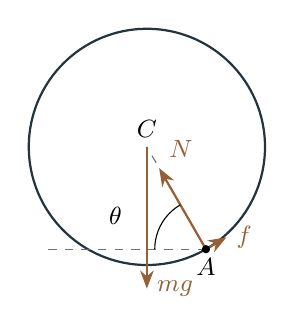
\begin{tikzpicture}[font=\small]
\coordinate(A)at(0,0);\coordinate(C)at(-.75,1.299038106);
\draw[object](C)circle(1.5);\draw[guide](A)--(C);
\draw[force](A)--(-.594653348,1.029969812)node[above right]{$N$};
\draw[force](A)--(.259807621,.15)node[right]{$f$};
\draw[force](C)--++(0,-1.8)node[right]{$mg$};
\draw[guide](A)--(-2,0);\draw(-.65,0)arc(180:120:.65);
\node at(-1.15,.42){$\theta$};\fill(A)circle(1.5pt)node[below]{$A$};
\node[above]at(C){$C$};
\end{tikzpicture}
\figcaption{解图6.6B\quad 径向支持力朝外，摩擦沿上翻切线向右上；示例$\theta=60^\circ,q=0.56$。}
\end{minipage}\end{center}
解图6.6B的径向方程为 $mg\sin\theta-N=mR\omega_\theta^2$。代入能量结果：
\[
 N=\frac73mg\sin\theta-\frac43mg\left(1-\frac hR\right)
 -\frac{mk^2v_0^2}{R}.
\]
上翻过程中 $\sin\theta$ 增加，故 $N$ 在初态最小：
\[
 N_{\min}=mg\left(1-\frac hR\right)-\frac{mk^2v_0^2}{R}>0.
\]
与过顶条件合并，
\[
 \result{\frac{12gR^2h}{(3R-2h)^2}<v_0^2<
 \frac{9gR^2(R-h)}{(3R-2h)^2}.}
\]
区间非空要求 $12h<9(R-h)$，即
\[\result{0<h<\frac37R.}\]
下界等号只到顶而不能继续，严格正接触取上界也为严格不等号。摩擦足够大还须足以提供切向需求 $|f|=mg|\cos\theta|/3$，即 $|f|\le\mu N$；若逼近零支持力的上界，所需摩擦系数会很大。

上述速度范围对应圆柱全程接触角点 $A$、无滑上翻并越过顶部的路径。
\subsubsection*{台阶碰撞的冲量与地面接触点的离地速度}
解图6.6C另画出碰撞瞬间的几何。记初始地面接触点为$B$，
令$d=\sqrt{2Rh-h^2}$，则相对角点$A$有
$\overrightarrow{AC}=(-d,R-h)$，且$d^2+(R-h)^2=R^2$。
碰前质心速度水平向右，自转顺时针；二者关于$A$的角动量同向，
平动项 $mv_0(R-h)$ 与自转项 $I_Cv_0/R$ 均取同一正号。
逐项代入得到
\[
mv_0(R-h)+\frac12mR^2\frac{v_0}{R}
=mv_0\left(\frac32R-h\right)
=\frac32mR^2\omega,
\]
\[
\omega=\frac{v_0(3R-2h)}{3R^2}.
\]
台阶处的法向和切向冲量都通过$A$；重力冲量矩可略。
地面接触点的作用也可能达到冲量量级。先按地面冲量为零求碰后运动，再由接触材料点的竖直速度判断地面是否需要施加冲量。
\begin{center}\begin{minipage}{\linewidth}\centering
\begin{tikzpicture}
\coordinate(A)at(0,0);\coordinate(C)at(-1.2,.9);\coordinate(B)at(-1.2,-.6);
\draw[object](-3.3,-.6)--(0,-.6)--(A)--(3,0);
\draw[object](C)circle(1.5);\draw[guide](C)--(A);\draw[guide](C)--(B);
\draw[force](A)--(-.96,.72)node[above left]{$J_n$};
\draw[force](A)--(.12,.16);\draw[guide](.14,.16)--(.5,.45);
\node[right]at(.5,.45){$J_t$};
\draw[motion](C)--++(.8,0)node[above]{$v_0$};
\draw[motion](B)--++(0,.65)node[left]{$v_{B,y}^+>0$};
\fill(A)circle(1.5pt)node[below right]{$A$};
\fill(B)circle(1.5pt)node[below]{$B$};\node[above left]at(C){$C$};
\node[align=left,anchor=west]at(1.2,1.8){$J_B=0$的候选解\\$B$点碰后向上离地};
\end{tikzpicture}
\figcaption{解图6.6C\quad 示例$h/R=0.4$；台阶两冲量在$A$作用，$B$点碰后的竖直速度给出离地方向。}
\end{minipage}\end{center}
若碰后绕$A$转动，质心速度为
\[
\vect v_C^+=\omega(R-h,d).
\]
初始位于最下方的材料点$B$，相对质心的位置为$(0,-R)$。
加上顺时针自转的速度后，
\[
\vect v_B^+=(-\omega h,\omega d).
\]
在本题最终得到的$0<h<3R/7$范围内，$d>0,\omega>0$，
所以$B$点竖直速度为正，立即向上离开地面，零地面冲量与单侧接触相容。
若题设改为地面在碰撞中也施加冲量，关于角点的角动量变化应计入该冲量的力矩。

台阶冲量的大小和方向由质心动量变化确定。
记$\eta=h/R$、$s=d/R=\sqrt{2\eta-\eta^2}$，
接触法线向外为$\vect n=(-s,1-\eta)$，上翻切线为
$\vect t=(1-\eta,s)$。投影可得
\[
J_n=mv_0s>0,\qquad J_t=\frac13mv_0\eta>0.
\]
因而碰撞所需的切向冲量沿上翻切线，
无滑捕获至少需$\mu\geq J_t/J_n=\eta/(3s)$。
这个冲量比描述碰撞瞬间的无滑捕获。随后绕角点运动时，静摩擦条件由各位置的切向力和支持力之比给出。

\subsubsection*{上翻受力的方向与完整速度窗口}
解图6.6B取$\theta$从左向水平线转向$AC$，
$\vect n=(-\cos\theta,\sin\theta)$沿$A\to C$，
$\vect t=(\sin\theta,\cos\theta)$沿质心上翻方向。
角速度为正，重力却使上翻减速。绕$A$及沿切线的方程是
\[
I_A\ddot\theta=-mgR\cos\theta,
\qquad f-mg\cos\theta=mR\ddot\theta.
\]
由此$\ddot\theta=-2g\cos\theta/(3R)$，
\[
f=\frac13mg\cos\theta>0\qquad(\theta_i\leq\theta<\pi/2).
\]
摩擦沿上翻切线向右上方，
它对圆柱质心产生使顺时针自转减速的力矩。
法向方程仍为$mg\sin\theta-N=mR\dot\theta^2$，
其中重力向内分量的一部分提供向心加速度，余下才由正压力平衡。

将能量式展开成不含缩写的形式，有
\[
\dot\theta^2=\frac{4g(R-h)}{3R^2}
-\frac{4g\sin\theta}{3R}
+\left(1-\frac{2h}{3R}\right)^2\frac{v_0^2}{R^2}.
\]
初态$\sin\theta_i=1-h/R$，过顶为$\sin\theta=1$。
角速度平方沿上翻减小，顶部速度为正给出整个过程的能量下限；法向压力随 $\sin\theta$ 增大，最小压力位于碰后起点。
过顶条件用顶部的速度，接触条件用起点的压力，分别取两项在上翻途中的最小值。

仍用$k=1-2\eta/3$，并定义
$q=k^2v_0^2/(gR)$，两项严格条件可写成
\[
\frac43\eta<q<1-\eta.
\]
解图6.6D直接画出这两条临界线；竖直截线在阴影内有长度，才存在允许速度。
\begin{center}\begin{minipage}{\linewidth}\centering
\begin{tikzpicture}[x=7cm,y=3.2cm]
\fill[accent!12](0,0)--(0,1)--(.428571429,.571428571)--cycle;
\draw[axis](0,0)--(.59,0)node[right]{$\eta=h/R$};
\draw[axis](0,0)--(0,1.2)node[above]{$q=k^2v_0^2/(gR)$};
\draw[thick,color=warm](0,1)--(.55,.45)node[right]{$1-\eta$};
\draw[traj](0,0)--(.55,.733333333)node[right]{$4\eta/3$};
\draw[guide](.428571429,0)--(.428571429,.571428571);
\node[below]at(.428571429,0){$3/7$};\node[left]at(0,1){$1$};
\draw[<->](.2,.266666667)--(.2,.8)node[midway,right]{允许速度};
\fill(.428571429,.571428571)circle(1.2pt);
\end{tikzpicture}
\figcaption{解图6.6D\quad 阴影内部同时满足过顶能量与正压力；两条临界线相交时速度窗口消失。}
\end{minipage}\end{center}
窗口非空等价于$4\eta/3<1-\eta$，即$7\eta<3$。
再把$q$换回$v_0^2$就得到前面的两个速度界限，
质量约去，每个速度平方的量纲均为$gR$。
下界等号对应顶部速度趋零，严格理想运动不能穿过最高位置继续前进；
上界等号使起点压力为零而切向需求仍为正，有限摩擦无法维持无滑接触。

题设的摩擦足够大也可化为具体条件。
上翻时$\cos\theta$减小、$N$增加，所以$f/N$在起点最大，
\[
\mu\geq\frac{f_i}{N_i}
=\frac{s}{3(1-\eta-q)}.
\]
若$\mu$给定且有限，速度上界应相应收紧为
\[
\frac43\eta<q\leq1-\eta-\frac{s}{3\mu},
\]
且右端大于左端时，允许区间非空。
这说明题设“足够大”是对所选速度而言；越靠近零压力上界，所需系数越大。
解图6.6A—C的几何统一为$R=1.5,h=0.6$；
受力示例取$q=0.56$，处于$0.533333\ldots<q<0.6$内，
相应全过程摩擦需$\mu\geq20/3$。
速度落在这个窗口且所需静摩擦可由接触提供时，圆柱沿角点的圆弧越过顶部。


\Needspace{18\baselineskip}

\pdfbookmark[2]{第 7 题 地月系统角动量与月球退行}{q7}

\section*{第 7 题\quad 地月系统角动量与月球退行}

\tagline{M-06-07}

如图,地球和月球的质量分别为\(M_{\mathrm{E}}\)和\(M_{\mathrm{m}}\),两者中心的距离用\(r\)表示,月球可看作质点．设地球的自转轴和月球绕地球作圆周运动的转轴重合，都通过地球中心，地球和月球的角速度分别为
\(\omega_{E}\) 和 \(\omega_{m}\)
．由于潮汐运动，地球自转角速度会发生微小变化，从而地球和月球的间距以及地球和月球系统的总能量也将发生变化．

1.试证明,地球和月球间距的时间变化率 \(\dot{r}\)
与地球自转角速度的时间变化率 \(\dot{\omega}_{\mathrm{E}}\) 的关系为

\[
\dot{ r } = - \frac{ 2 \sqrt{ r } \; I_{ E } } { M_{ \mathrm{m} } \sqrt{ G M_{ E } } } \dot{ \omega }_{ E }
\]

式中 \(I_{\mathrm{E}}\) 是地球对自转轴的转动惯量, \(G\) 是引力常量.

试导出地球和月球系统机械能时间变化率的表达式.

设现在的地球与月球间距为 \(r(0)\), 地球的自转角速度为
\(\omega_{\mathrm{E}}(0)\), 受扰动后相应的量变为 \(r(t)\) 和
\(\omega_{\mathrm{E}}(t)\), 因扰动很小, 月球仍作圆周运动. 试证明

\[
\omega_{ \mathrm{E} } ( t ) = \omega_{ \mathrm{E} } ( 0 ) - \frac{ M_{ \mathrm{m} } \sqrt{ G M_{ \mathrm{E} } } } { I_{ \mathrm{E} } } [ \sqrt{ r ( t ) } - \sqrt{ r ( 0 ) } ]
\]

已知
\(G=6.672 \times 10^{-11} \mathrm{N} \cdot \mathrm{m}^{2} / \mathrm{kg}^{2}, M_{\mathrm{E}}=5.89 \times 10^{24} \mathrm{kg}, M_{\mathrm{m}}=7.34 \times 10^{22} \mathrm{kg}, r=3.84 \times 10^{8} \mathrm{m}\),
\(R_{\mathrm{E}}=6.37 \times 10^{6} \mathrm{m}\) (地球半径).
试计算地球和月球间距增加 2\% 时, 地球日将变成多少小时.

数值计算将地球视为均匀实心球，初始自转周期取 \(24\,\mathrm h\)。

\begin{center}\begin{minipage}{\linewidth}\centering
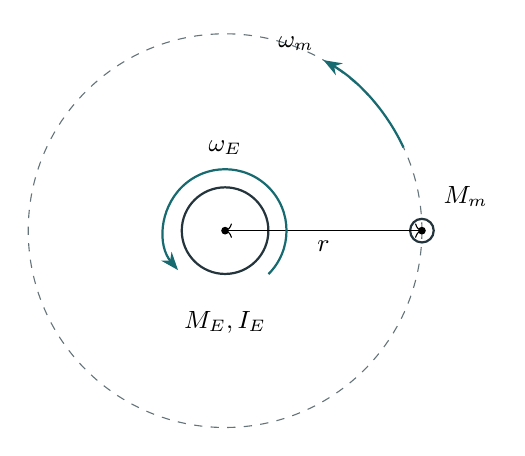
\begin{tikzpicture}[font=\small]
\draw[guide](0,0)circle(2.5);\draw[object](0,0)circle(.55);
\draw[object](2.5,0)circle(.15);\fill(0,0)circle(1.4pt);\fill(2.5,0)circle(1.4pt);
\draw[<->](0,0)--(2.5,0)node[midway,below]{$r$};
\draw[motion](.551543289,-.551543289)arc(-45:220:.78);
\draw[motion](2.265769467,1.056545654)arc(25:60:2.5);
\node[below]at(0,-.9){$M_E,I_E$};
\node[above right]at(2.65,.18){$M_m$};
\node at(0,1.05){$\omega_E$};
\node[above left]at(1.25,2.165063509){$\omega_m$};
\end{tikzpicture}
\figcaption{图 6.7\quad 示意自转与同向圆轨道；图的比例不用于数值计算。}
\end{minipage}\end{center}

\Needspace{5\baselineskip}\subsection*{解答}

\begin{center}\begin{minipage}{\linewidth}\centering
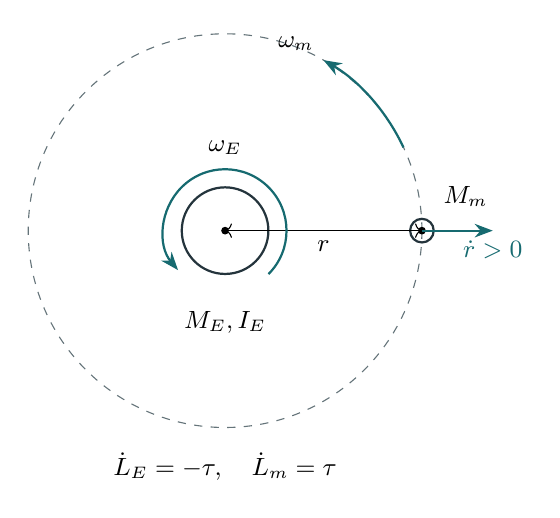
\begin{tikzpicture}[font=\small]
\draw[guide](0,0)circle(2.5);\draw[object](0,0)circle(.55);
\draw[object](2.5,0)circle(.15);\fill(0,0)circle(1.4pt);\fill(2.5,0)circle(1.4pt);
\draw[<->](0,0)--(2.5,0)node[midway,below]{$r$};
\draw[motion](.551543289,-.551543289)arc(-45:220:.78);
\draw[motion](2.265769467,1.056545654)arc(25:60:2.5);
\node[below]at(0,-.9){$M_E,I_E$};
\node[above right]at(2.65,.18){$M_m$};
\node at(0,1.05){$\omega_E$};
\node[above left]at(1.25,2.165063509){$\omega_m$};
\draw[motion](2.5,0)--(3.4,0)node[below]{$\dot r>0$};
\node at(0,-3){$\dot L_E=-\tau,\quad\dot L_m=\tau$};
\end{tikzpicture}
\figcaption{解图 6.7A\quad 轨道外移时公转角动量增加，自转角动量相应减少。}
\end{minipage}\end{center}
本题采用地球中心近似固定、月球为质点且始终沿近圆轨道变化的模型。解图6.7A中自转与公转轴重合、方向一致；外力矩忽略，所以
\[
 L=I_E\omega_E+M_mr^2\omega_m=\text{常量},\qquad
 \frac{GM_EM_m}{r^2}=M_mr\omega_m^2.
\]
因此 $\omega_m=\sqrt{GM_E/r^3}$、$L_m=M_m\sqrt{GM_Er}$。对总角动量求导，
\[
 I_E\dot\omega_E+\frac{M_m\sqrt{GM_E}}{2\sqrt r}\dot r=0,
 \qquad\result{\dot r=-\frac{2\sqrt r I_E}{M_m\sqrt{GM_E}}\dot\omega_E.}
\]
地球自转减慢时月球轨道半径增大。系统机械能包含自转、月球平动和引力势能，
\[
\begin{aligned}
 E&=\frac12I_E\omega_E^2+\frac12M_mr^2\omega_m^2-\frac{GM_EM_m}{r}\\
 &=\frac12I_E\omega_E^2-\frac{GM_EM_m}{2r},\\
 \dot E&=I_E\omega_E\dot\omega_E+\frac{GM_EM_m}{2r^2}\dot r\\
 &=-\frac{M_m}{2}\left(\omega_E\sqrt{\frac{GM_E}{r}}-\frac{GM_E}{r^2}\right)\dot r\\
 &=\result{I_E(\omega_E-\omega_m)\dot\omega_E}.
\end{aligned}
\]
在 $\omega_E>\omega_m$ 的退行情形，$\dot\omega_E<0$，所以机械能减少，差额转化为热。角动量在自转和轨道间转移，产生的热来自总机械能的减少。

将微分关系写成 $\dd\omega_E=-[M_m\sqrt{GM_E}/I_E]\dd\sqrt r$，从初态积分到时刻 $t$，
\[
 \result{\omega_E(t)=\omega_E(0)-\frac{M_m\sqrt{GM_E}}{I_E}
 [\sqrt{r(t)}-\sqrt{r(0)}].}
\]
数值部分使用题给均匀球近似 $I_E=2M_ER_E^2/5$，$T_0=24\,\mathrm h$，$\omega_E(0)=2\pi/T_0$。把半径增幅代入前，先保留无量纲系数：
\[
 \frac{\omega_E(t)}{\omega_E(0)}
 =1-\frac{M_m\sqrt{GM_Er(0)}}{I_E\omega_E(0)}(\sqrt{1.02}-1).
\]
按所给常量，系数约为 $4.10135$，角速度比约为 $0.9591895$，故
\[\result{T=\frac{24}{0.9591895}\,\mathrm h\approx25.021\,\mathrm h.}\]
计算中的 $r(0)=3.84\times10^8\,\mathrm m$ 是地月中心距离；模型忽略地球的绕共同质心公转、月球自转和地球内部密度差异。
\subsubsection*{月球轨道外移与潮汐耗散功率}
在本题地心近似、缓慢圆轨道演化的模型内，$I_E$取常量。
先用圆轨道关系消去$\omega_m$，再对角动量求导：
\[
\begin{aligned}
0&=I_E\dot\omega_E+M_m\frac{\dd}{\dd t}(r^2\omega_m)\\
&=I_E\dot\omega_E+M_m\sqrt{GM_E}\frac{\dd\sqrt r}{\dd t}\\
&=I_E\dot\omega_E+\frac{M_m\sqrt{GM_E}}{2\sqrt r}\dot r.
\end{aligned}
\]
将第一项移到右侧并解出半径变化率，分母为$\sqrt{GM_E}$。其中链式法则给$\dd\sqrt r/\dd t=\dot r/(2\sqrt r)$。在同一时间区间积分时，地球自转的端点取$\omega_E(0),\omega_E(t)$，月球轨道端点取$\sqrt{r(0)},\sqrt{r(t)}$，由此连接两项的有限改变量。

把流入月球轨道的角动量率记为$\tau=\dot L_m=-I_E\dot\omega_E$。
解图6.7A的轨道外移箭头对应$\tau>0$。
轨道能量$E_m=-GM_EM_m/(2r)$与轨道角动量满足
\[
\frac{\dd E_m}{\dd r}=\frac{GM_EM_m}{2r^2},
\quad
\frac{\dd L_m}{\dd r}=\frac{M_m\sqrt{GM_E}}{2\sqrt r},
\quad
\frac{\dd E_m}{\dd L_m}=\omega_m.
\]
所以地球自转损失能量的速率是$\omega_E\tau$，
月球轨道增加能量的速率是$\omega_m\tau$，两者的差转为热：
\[
\dot E_E=-\omega_E\tau,\qquad
\dot E_m=\omega_m\tau,\qquad
\dot Q=\tau(\omega_E-\omega_m)=-\dot E.
\]
本题中轨道获得的能量小于地球自转失去的能量，其差为热。若行星自转慢于公转，耗散仍要求热产生率为正，转矩方向随角速度差反转，轨道半径的变化率$\dot r$也随之反号。

\subsubsection*{日长计算的单位与有限比值}
按题给常量逐项代入，初始量为
\[
I_E=\frac25(5.89\times10^{24})(6.37\times10^6)^2
=9.55991764\times10^{37}\,\mathrm{kg\,m^2},
\]
\[
T_0=24\times3600\,\mathrm s=86400\,\mathrm s,
\quad \omega_E(0)=7.27220522\times10^{-5}\,\mathrm{s^{-1}},
\]
\[
\omega_m(0)=2.63444314\times10^{-6}\,\mathrm{s^{-1}}.
\]
自转确比公转快，符合前面的耗散符号判断。
将公转角动量与初始自转角动量之比记为
\[
C=\frac{M_m\sqrt{GM_Er(0)}}{I_E\omega_E(0)}=4.101352163\ldots.
\]
因为月球轨道半径增加$2\%$，公转角动量只增加
$\sqrt{1.02}-1$倍；转移量占地球初始自转角动量的比例则为
\[
\frac{\Delta L_m}{I_E\omega_E(0)}
=C(\sqrt{1.02}-1)=0.04081047942\ldots.
\]
地球角速度剩余$0.9591895206$倍，因此应取它的倒数求周期，
相应周期比为 $1/0.9591895206$。
解图6.7B按同一有限比值绘制，标出$2\%$处的日长。
\begin{center}\begin{minipage}{\linewidth}\centering
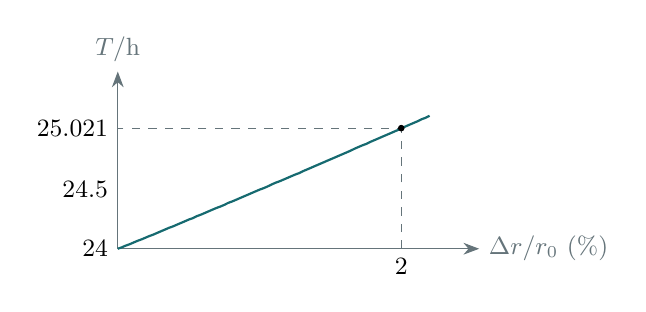
\begin{tikzpicture}[x=1.8cm,y=1.5cm]
\draw[axis](0,0)--(2.55,0)node[right]{$\Delta r/r_0\ (\%)$};
\draw[axis](0,0)--(0,1.5)node[above]{$T/\mathrm h$};
\draw[traj,domain=0:2.2,samples=80]plot(\x,{24/(1-4.101352163*(sqrt(1+\x/100)-1))-24});
\draw[guide](2,0)--(2,1.021124069)--(0,1.021124069);
\fill(2,1.021124069)circle(1.2pt);
\node[below]at(2,0){$2$};\node[left]at(0,0){$24$};
\node[left]at(0,.5){$24.5$};\node[left]at(0,1.021124069){$25.021$};
\end{tikzpicture}
\figcaption{解图6.7B\quad 横坐标为半径增幅的百分数，纵坐标按日长标数；曲线使用精确周期比。}
\end{minipage}\end{center}
小增幅$\delta=\Delta r/r_0$时，$\sqrt{1+\delta}-1\simeq\delta/2$，
故$\Delta T/T_0\simeq C\delta/2$，给出周期增加约百分之四的量级。
最终数值仍用有限比值，得到$25.0211241\,\mathrm h$。
此计算只由半径增幅和角动量守恒确定新日长，
达到该增幅所需的时间由潮汐耗散或转矩随状态变化的规律决定。


\Needspace{18\baselineskip}

\pdfbookmark[2]{第 8 题 行星自转与卫星圆轨道的角动量转移}{q8}

\section*{第 8 题\quad 行星自转与卫星圆轨道的角动量转移}

\tagline{M-06-08}

某行星相对其质心轴的转动惯量为 \(I\), 自转角速度为 \(\Omega\). 质量为
\(m\) 的卫星(可看作质点)绕该行星沿圆轨道运动, 轨道半径为 \(r\), 角速度为
\(\omega\), 假定两种角速度的方向一致.

一般情形下 \(\Omega\) 与 \(\omega\) 并不相等, 由于行星上的潮汐摩擦,
行星自转角速度将发生变化, 卫星的圆运动角速度也将相应地改变,
试求两种角速度的改变量之间的关系.

2.潮汐摩擦将引起行星与卫星系统机械能的损耗,试问在什么情形下系统机械能可达稳定值.

\begin{center}\begin{minipage}{\linewidth}\centering
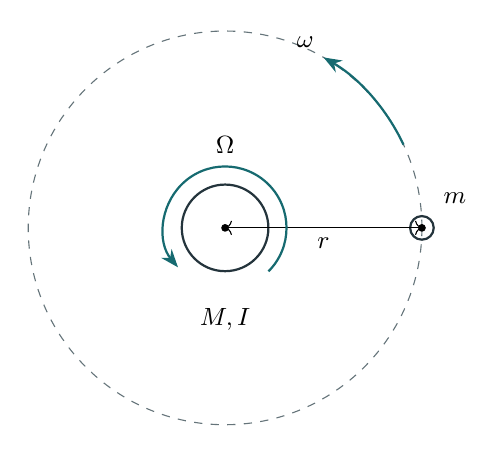
\begin{tikzpicture}[font=\small]
\draw[guide](0,0)circle(2.5);\draw[object](0,0)circle(.55);
\draw[object](2.5,0)circle(.15);\fill(0,0)circle(1.4pt);\fill(2.5,0)circle(1.4pt);
\draw[<->](0,0)--(2.5,0)node[midway,below]{$r$};
\draw[motion](.551543289,-.551543289)arc(-45:220:.78);
\draw[motion](2.265769467,1.056545654)arc(25:60:2.5);
\node[below]at(0,-.9){$M,I$};
\node[above right]at(2.65,.18){$m$};
\node at(0,1.05){$\Omega$};
\node[above left]at(1.25,2.165063509){$\omega$};
\end{tikzpicture}
\figcaption{图 6.8\quad 行星自转与卫星圆轨道之间转移角动量。}
\end{minipage}\end{center}

\Needspace{5\baselineskip}\subsection*{解答}

\begin{center}\begin{minipage}{\linewidth}\centering
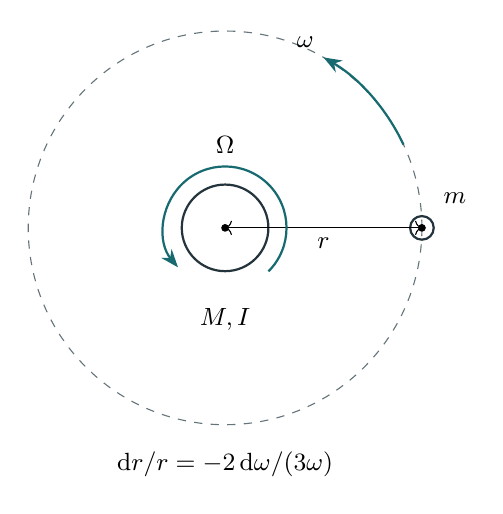
\begin{tikzpicture}[font=\small]
\draw[guide](0,0)circle(2.5);\draw[object](0,0)circle(.55);
\draw[object](2.5,0)circle(.15);\fill(0,0)circle(1.4pt);\fill(2.5,0)circle(1.4pt);
\draw[<->](0,0)--(2.5,0)node[midway,below]{$r$};
\draw[motion](.551543289,-.551543289)arc(-45:220:.78);
\draw[motion](2.265769467,1.056545654)arc(25:60:2.5);
\node[below]at(0,-.9){$M,I$};
\node[above right]at(2.65,.18){$m$};
\node at(0,1.05){$\Omega$};
\node[above left]at(1.25,2.165063509){$\omega$};
\node at(0,-3){$\dd r/r=-2\dd\omega/(3\omega)$};
\end{tikzpicture}
\figcaption{解图 6.8A\quad 圆轨道角速度与半径满足 $r\propto\omega^{-2/3}$。}
\end{minipage}\end{center}
解图6.8A中，轨道半径随公转角速度一同演化，角动量 $L=I\Omega+mr^2\omega$ 的微分包含 $r$ 和两个角速度的变化。圆轨道条件给 $\omega^2=GM/r^3$，微分得
\[
 2\omega\dd\omega=-3GM r^{-4}\dd r,
 \quad \frac{\dd r}{\dd\omega}=-\frac{2r}{3\omega}.
\]
再由角动量守恒：
\[
\begin{aligned}
 0=\dd L&=I\dd\Omega+mr^2\dd\omega+2mr\omega\dd r\\
 &=I\dd\Omega-\frac13mr^2\dd\omega,
 \qquad\result{\frac{\dd\Omega}{\dd\omega}=\frac{mr^2}{3I}.}
\end{aligned}
\]
总机械能为 $E=I\Omega^2/2+mr^2\omega^2/2-GMm/r$。各变量都微分，并用圆轨道关系将最后一项改写成 $mr\omega^2\dd r$：
\[
\begin{aligned}
 \dd E&=I\Omega\dd\Omega+2mr\omega^2\dd r+mr^2\omega\dd\omega\\
 &=\left[\frac13mr^2\Omega-\frac43mr^2\omega+mr^2\omega\right]\dd\omega\\
 &=\frac13mr^2(\Omega-\omega)\dd\omega.
\end{aligned}
\]
耗散可停止的同步条件为 $\Omega=\omega$。此时相对于行星表面的潮汐形状不再周期移动，在本题理想化模型下没有持续潮汐耗散。

固定总角动量下，能量在同步状态附近的变化由二阶导数给出：
\[
 \left.\frac{\dd^2E}{\dd\omega^2}\right|_{\Omega=\omega}
 =\frac{mr^2}{3}\left(\frac{mr^2}{3I}-1\right).
\]
求这个二阶导数时，沿固定 $L$ 的路径将
$\dd E/\dd\omega=(mr^2/3)(\Omega-\omega)$ 再求导：
\[
 \frac{\dd^2E}{\dd\omega^2}
 =\frac{2mr}{3}\frac{\dd r}{\dd\omega}(\Omega-\omega)
 +\frac{mr^2}{3}\left(\frac{\dd\Omega}{\dd\omega}-1\right).
\]
同步点使第一项消失，第二项中再代入 $\dd\Omega/\dd\omega=mr^2/(3I)$，才得到前式。求导中同时使用 $r(\omega)$ 和 $\Omega(\omega)$ 的关系。

所以稳定同步支还须 $mr^2>3I$；$mr^2<3I$ 的同步点是极大值。等号处两支合并，二阶导数为零；该点的高阶变化在下面由同一个能量函数求出。
\subsubsection*{全部变量微分与固定角动量路径}
设行星质量为$M$，在行星中心近似固定、卫星近圆演化的模型内，
$r$随$\omega$变化，$\Omega$也由守恒角动量决定。
从圆轨道关系微分后保留尚未约去的$r$次方，可得
\[
\frac{\dd r}{\dd\omega}
=-\frac{2\omega r^4}{3GM}
=-\frac{2r}{3\omega}.
\]
角动量微分中的两项公转贡献分别为
$mr^2\dd\omega$和$2mr\omega\dd r$，代入后后者为
$-4mr^2\dd\omega/3$，故它们的总和是
$-mr^2\dd\omega/3$。
因此行星自转与卫星公转的角速度改变量同号，
而轨道半径改变量与它们反号；系数$mr^2/(3I)$无量纲。

能量在使用圆轨道条件以前的完整微分是
\[
\dd E=I\Omega\dd\Omega
+mr\omega^2\dd r+mr^2\omega\dd\omega
+\frac{GMm}{r^2}\dd r.
\]
引力势能的微分项与平动动能的半径项同号，
用$GM/r^2=r\omega^2$合并后才成为$2mr\omega^2\dd r$。
沿固定$L$的路径可写成
\[
\frac{\dd E}{\dd\omega}
=I\Omega\frac{\dd\Omega}{\dd\omega}
+2mr\omega^2\frac{\dd r}{\dd\omega}+mr^2\omega
=\frac{mr^2}{3}(\Omega-\omega).
\]
若$\Omega>\omega$，耗散方向应有$\dd\omega<0$，
于是$\dd\Omega<0,\dd r>0$；若$\Omega<\omega$，方向相反。
两种情形均使$\dd E<0$。
同步使这一阶变化为零，只说明潮汐形状相对行星表面静止，
是否有能量极小仍由二阶及退化时的高阶变化决定。

\subsubsection*{两条同步支何时存在}
消去$\Omega$，固定总角动量下的能量函数为
\[
\Omega(r)=\frac{L-m\sqrt{GMr}}{I},\qquad
E(r)=\frac{[L-m\sqrt{GMr}]^2}{2I}-\frac{GMm}{2r}.
\]
同步时$\Omega=\sqrt{GM/r^3}$，相应所需总角动量为
\[
L_s(r)=\sqrt{GM}\left(Ir^{-3/2}+mr^{1/2}\right),
\]
\[
L_s'(r)=\frac{\sqrt{GM}}{2r^{5/2}}(mr^2-3I).
\]
所以$r_c=\sqrt{3I/m}$处有唯一最小值
\[
L_c=L_s(r_c)=\frac43m\sqrt{GM r_c}.
\]
当$L>L_c$时有内外两个同步半径；
内支$mr^2<3I$对应能量极大，外支$mr^2>3I$对应能量极小。
当$L<L_c$时没有同步圆轨道候选。
作为卫星轨道，所得半径还取行星表面以外的值。

为把稳定性画成真实能量曲线，令$x=r/r_c$、
$\ell=L/[m\sqrt{GM r_c}]$、$e=E/[GMm/(2r_c)]$，则
\[
e(x)=3(\ell-\sqrt x)^2-\frac1x.
\]
解图6.8B取$\ell=1.5>4/3$，
两个驻值在$x\simeq0.593018,1.878302$，分别是极大与极小。
\begin{center}\begin{minipage}{\linewidth}\centering
\begin{tikzpicture}[x=2.5cm,y=3cm]
\draw[axis](0,0)--(2.4,0)node[right]{$x=r/r_c$};
\draw[axis](0,-.8)--(0,.16)node[above]{$e$};
\draw[traj,domain=.3:2.2,samples=130]plot(\x,{3*(1.5-sqrt(\x))^2-1/\x});
\fill(.593017518,-.087925031)circle(1.2pt);
\fill(1.878302350,-.482093999)circle(1.2pt);
\draw[guide](.593017518,0)--(.593017518,-.087925031);
\draw[guide](1.878302350,0)--(1.878302350,-.482093999);
\node[above]at(.593017518,-.045){内支：极大};
\node[below]at(1.878302350,-.56){外支：极小};
\node[left]at(0,-.5){$-0.5$};
\end{tikzpicture}
\figcaption{解图6.8B\quad 固定$\ell=1.5$的精确能量曲线；耗散能停留在外侧极小附近，内侧极大不稳定。}
\end{minipage}\end{center}
当$L=L_c$，两个同步点合并于$r_c$。
二阶导数为零还不够判断，此处沿同一固定$L$的能量函数有
\[
E'(r_c)=E''(r_c)=0,\qquad
E^{\prime\prime\prime}(r_c)=\frac{3GMm}{2r_c^4}>0.
\]
因此首个非零变化是立方项，在$r_c$两侧异号，
能量在临界点的一侧降低、另一侧升高，该点为水平拐点。稳定同步取严格的 $mr^2>3I$。


\Needspace{18\baselineskip}

\pdfbookmark[2]{第 9 题 线轴受拉时的滚动方向与加速度}{q9}

\section*{第 9 题\quad 线轴受拉时的滚动方向与加速度}

\tagline{M-06-09}

如图,一线轴质量为\(m\),绕质心轴的转动惯量为\(I\),大小半径分别为\(R\)和\(r\),轴上绕线,

以力 \(F\) 拉线,拉力方向与水平面的夹角用 \(\theta\) 表示.
线轴放置在水平桌面上,与桌面之间的摩擦系数为
\(\mu\),试讨论线轴的运动情况.

\begin{center}\begin{minipage}{\linewidth}\centering
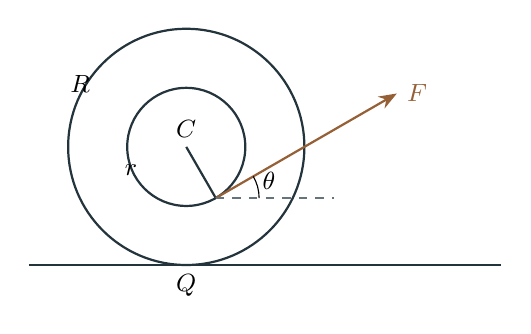
\begin{tikzpicture}[font=\small]
\draw[object](-2,-1.5)--(4,-1.5);\draw[object](0,0)circle(1.5);\draw[object](0,0)circle(.75);\coordinate(P)at(.375,-.649519053);\draw[object](0,0)--(P);\draw[force](P)--++(2.3,1.327905619)node[right]{$F$};\draw[guide](P)--++(1.5,0);\draw (.925,-.649519053)arc(0:30:.55);\node at(1.05,-.43){$\theta$};\node[above]at(0,0){$C$};\node[left]at(-1.1,.8){$R$};\node[left]at(-.5,-.3){$r$};\node[below]at(0,-1.5){$Q$};
\end{tikzpicture}
\figcaption{图 6.9\quad 拉线与内轴下侧相切；$Q$ 为桌面接触点。}
\end{minipage}\end{center}

\Needspace{5\baselineskip}\subsection*{解答}

\begin{center}\begin{minipage}{\linewidth}\centering
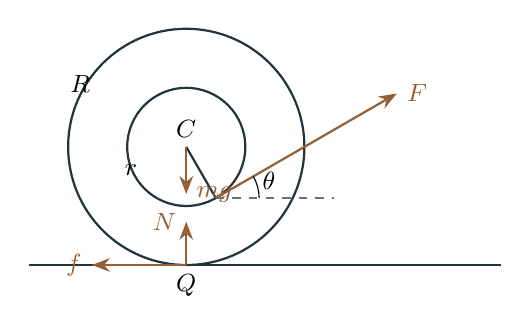
\begin{tikzpicture}[font=\small]
\draw[object](-2,-1.5)--(4,-1.5);\draw[object](0,0)circle(1.5);\draw[object](0,0)circle(.75);\coordinate(P)at(.375,-.649519053);\draw[object](0,0)--(P);\draw[force](P)--++(2.3,1.327905619)node[right]{$F$};\draw[guide](P)--++(1.5,0);\draw (.925,-.649519053)arc(0:30:.55);\node at(1.05,-.43){$\theta$};\node[above]at(0,0){$C$};\node[left]at(-1.1,.8){$R$};\node[left]at(-.5,-.3){$r$};\node[below]at(0,-1.5){$Q$};\draw[force](0,-1.5)--(-1.2,-1.5)node[left]{$f$};\draw[force](0,-1.5)--(0,-.95)node[left]{$N$};\draw[force](0,0)--(0,-.6)node[right]{$mg$};
\end{tikzpicture}
\figcaption{解图 6.9A\quad $N$由接触点$Q$竖直向上，$mg$从质心向下；两根箭头分段画开。}
\end{minipage}\end{center}
线从内轴下方切向引出，解图6.9A的拉力对质心产生逆时针力矩 $Fr$。取向右平移和顺时针转动为正，$f$ 表示向左摩擦力的大小，且 $0\le\theta\le\pi/2$。

先假设静止起动后纯滚。竖直、水平、绕质心与无滑条件为
\[
 N=mg-F\sin\theta,\quad ma=F\cos\theta-f,\quad
 I\beta=fR-Fr,\quad a=R\beta.
\]
消去 $f,\beta$，
\[
\begin{aligned}
 a&=\frac{FR(R\cos\theta-r)}{I+mR^2},&
 \beta&=\frac{F(R\cos\theta-r)}{I+mR^2},\\
 f&=\frac{F(mRr+I\cos\theta)}{I+mR^2},&
 N&=mg-F\sin\theta.
\end{aligned}
\]
$f>0$，摩擦始终向左。$\cos\theta>r/R$ 时向右滚；小于时向左滚；等于时 $a=\beta=0$，从静止保持不动。接地和不滑动条件分别是
\[
 N>0,\qquad\mu\ge\mu_{\min}
 =\frac{F(mRr+I\cos\theta)}{(I+mR^2)(mg-F\sin\theta)}.
\]

\Needspace{14\baselineskip}
当 $\mu<\mu_{\min}$，静止起动后的接触点向右滑，取动摩擦与题给系数相同，$f=\mu N$。独立列平移、转动方程，得到
\[
\begin{aligned}
 a&=\frac{F\cos\theta-\mu(mg-F\sin\theta)}m,\\
 \beta&=\frac{\mu R(mg-F\sin\theta)-Fr}{I}.
\end{aligned}
\]
从静止起动时，接触点加速度 $a_s=a-R\beta$ 决定随后滑速的方向：
\[
 a_s=F\left(\frac{\cos\theta}{m}+\frac{Rr}{I}\right)
 -\mu N\left(\frac1m+\frac{R^2}{I}\right)>0.
\]
底点右滑时质心加速度仍须独立判断。平移方向由 $F\cos\theta-\mu N$ 的符号决定，转动方向由 $\mu NR-Fr$ 的符号决定；在大拉线角时，质心仍可能向左加速而接触点向右滑。已有初速度时，先算接触点当时的滑速，再按其反向取动摩擦。
\subsubsection*{接触点力矩与纯滚方向}
在解图6.9A的几何中，$CP=r$且$CP\perp F$，
拉线从内轴下侧引出；$Q$在质心正下方，$CQ=R$。
拉力关于$Q$的顺时针力矩为
\[
M_Q=F(R\cos\theta-r).
\]
纯滚从静止起动时，$I_Q=I+mR^2$，故
$\beta=M_Q/(I+mR^2)$，再由$a=R\beta$还原前面的结果。
拉力作用线经过 $Q$ 的哪一侧，决定力矩的转动方向及纯滚起动方向。
在$\theta_* =\arccos(r/R)$处，拉力作用线通过$Q$，
解图6.9B将这条直线延长到接触点；它对$Q$的力矩为零。
\begin{center}\begin{minipage}{\linewidth}\centering
\begin{tikzpicture}
\draw[object](-2,-1.5)--(3,-1.5);\draw[object](0,0)circle(1.5);
\draw[object](0,0)circle(.75);\coordinate(P)at(.649519053,-.375);
\coordinate(Q)at(0,-1.5);\draw[guide](Q)--(P);
\draw[force](P)--(1.399519053,.924038106)node[right]{$F$};
\draw[guide](0,0)--(P);\fill(P)circle(1.4pt)node[right]{$P$};
\fill(Q)circle(1.4pt)node[below]{$Q$};\node[above]at(0,0){$C$};
\node[align=left,anchor=west]at(2,.7){$r/R=1/2$\\$\theta_*=60^\circ$\\拉力作用线通过$Q$};
\end{tikzpicture}
\figcaption{解图6.9B\quad 纯滚临界方向由接触点矩决定；静止平衡所需摩擦取 $f=F\cos\theta_*$。}
\end{minipage}\end{center}
此时从静止保持平衡所需$f=F\cos\theta_*$，
摩擦仍向左并与拉力的水平分量平衡。由$f\leq\mu N$可进一步得
\[
F\leq\frac{\mu mg}{r/R+\mu\sqrt{1-r^2/R^2}}.
\]
这个条件同时保证压力为正。
对一般角度还须保留$N=mg-F\sin\theta>0$；
$\theta=0$时没有由拉力竖直分量导致的离地上限，
此时 $N=mg$，支持力与拉力大小无关。

\subsubsection*{线轴质心、自旋与接触点的三个运动方向}
以$\mu$同时表示题设采用的静、动摩擦系数，
在从静止起动、静摩擦不足的分支中，令
\[
\rho=\frac rR,\quad \kappa=\frac{I}{mR^2},\quad
c=\cos\theta,\quad q=\frac{\mu N}{F}.
\]
纯滚所需的$f/F$为$q_s=(\rho+\kappa c)/(1+\kappa)$。
摩擦不足即$q<q_s$，代入两条独立动力学方程可写成
\[
a=\frac Fm(c-q),\qquad
R\beta=\frac{F}{m\kappa}(q-\rho),
\]
\[
a_s=a-R\beta
=\frac{F(1+\kappa)}{m\kappa}(q_s-q)>0.
\]
从零滑速出发，正的接触点加速度使接触点向右滑，动摩擦因而向左。
但质心向右或向左分别由$q<c$或$q>c$决定，
自旋顺时针或逆时针分别由$q>\rho$或$q<\rho$决定。
在前一等式处质心加速度为零，在后一等式处角加速度为零，两种运动各由对应的比较式决定。
若起初已有接触滑速$u_0$，动摩擦方向由当前的$u=v-R\omega$决定。从$u_0=0$起动时，接触点水平加速度$a_s$决定随后滑速的正负。

取$\theta=75^\circ,\rho=1/2,\kappa=1/2,F=0.4mg,\mu=0.2$，
有$N=0.61362967mg>0$、$\mu_{\min}=0.27352416>\mu$。
两加速度及接触点加速度分别为
\[
\frac ag=-0.01919832,\qquad
\frac{R\beta}{g}=-0.15454813,\qquad
\frac{a_s}{g}=0.13534982.
\]
解图6.9C同时标出三种方向：质心向左加速、线轴逆时针加速自旋，
接触点却向右滑。摩擦只与最后这个相对滑动方向相反。
\begin{center}\begin{minipage}{\linewidth}\centering
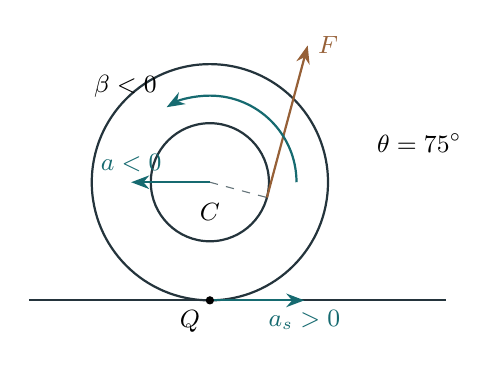
\begin{tikzpicture}
\draw[object](-2.3,-1.5)--(3,-1.5);\draw[object](0,0)circle(1.5);
\draw[object](0,0)circle(.75);\coordinate(P)at(.724444370,-.194114284);
\draw[force](P)--(1.242082460,1.737737369)node[right]{$F$};
\draw[guide](0,0)--(P);\draw[motion](0,0)--(-1,0)node[above]{$a<0$};
\draw[motion](1.1,0)arc(0:120:1.1);
\node[above left]at(-.55,.952627944){$\beta<0$};
\draw[motion](0,-1.5)--(1.2,-1.5)node[below]{$a_s>0$};
\fill(0,-1.5)circle(1.5pt)node[below left]{$Q$};
\node[below]at(0,-.15){$C$};\node[right]at(2,.5){$\theta=75^\circ$};
\end{tikzpicture}
\figcaption{解图6.9C\quad 同一滚滑分支的三个运动方向；逆时针角加速度按所取顺时针正向记为负。}
\end{minipage}\end{center}


\Needspace{18\baselineskip}

\pdfbookmark[2]{第 10 题 斜面木块牵引实心圆柱体的滚动动力学}{q10}

\section*{第 10 题\quad 斜面木块牵引实心圆柱体的滚动动力学}

\tagline{M-06-10}

如图6.10,在\(\alpha=30^{\circ}\)的斜面上,质量\(m_{2}=4\ \mathrm{kg}\)的木块经轻绳与质量\(m_{1}=8\ \mathrm{kg}\)、半径\(r=5\ \mathrm{cm}\)的实圆柱体的转轴相连.已知斜面的摩擦系数\(\mu=0.2\),圆柱体轴承中的摩擦可以忽略.试求物体的加速度\(a\),并讨论加速度\(a\)、张力\(T\)、圆柱体所受摩擦力\(f_{1}\)随斜面倾角\(\alpha\)的变化.

讨论各倾角时，均取两物体从静止释放，静、动摩擦系数均取题给值。

\begin{center}\begin{minipage}{\linewidth}\centering
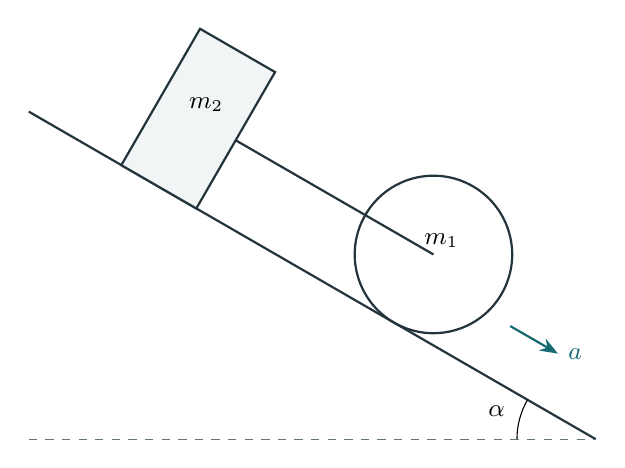
\begin{tikzpicture}[font=\small]
\draw[object](-3.6,2.08)--(3.6,-2.08);\begin{scope}[rotate=-30]\draw[object,fill=rulegray!30](-2.8,0)rectangle(-1.7,2);\draw[object](1.2,1)circle(1);\draw[object](-1.7,1)--(1.2,1);\node at(-2.25,1.2){$m_2$};\node at(1.2,1.2){$m_1$};\draw[motion](2.5,.7)--(3.2,.7)node[right]{$a$};\end{scope}\draw(2.6,-2.08)arc(180:150:1);\node at(2.34,-1.73){$\alpha$};\draw[guide](-3.6,-2.08)--(3.6,-2.08);
\end{tikzpicture}
\figcaption{图 6.10\quad 圆柱在下坡一侧，绳在轴心处牵引。}
\end{minipage}\end{center}

\Needspace{5\baselineskip}\subsection*{解答}

\begin{center}\begin{minipage}{\linewidth}\centering
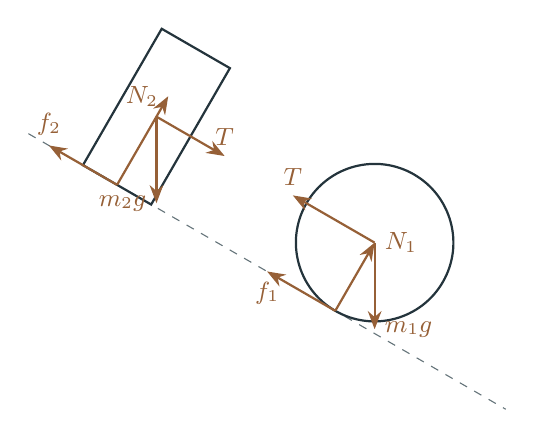
\begin{tikzpicture}[font=\small]
\begin{scope}[rotate=-30]\draw[guide](-3.5,0)--(3.5,0);\draw[object](-2.7,0)rectangle(-1.7,2);\draw[object](1,1)circle(1);\draw[force](-2.2,1)--++(1,0)node[above]{$T$};\draw[force](-2.2,0)--++(-1,0)node[above]{$f_2$};\draw[force](-2.2,0)--++(0,1.3)node[left]{$N_2$};\draw[force](1,1)--++(-1.2,0)node[above]{$T$};\draw[force](1,0)--++(-1,0)node[below]{$f_1$};\draw[force](1,0)--++(0,1)node[right]{$N_1$};\end{scope}\draw[force](-1.405,1.966)--++(0,-1.1)node[left]{$m_2g$};\draw[force](1.366,.366)--++(0,-1.1)node[right]{$m_1g$};
\end{tikzpicture}
\figcaption{解图 6.10A\quad 张力在两个物体上反向；两接触摩擦在下滚阶段均向上坡。}
\end{minipage}\end{center}
解图6.10A中圆柱在木块的下坡一侧，轻绳连两者的轴或质心。木块受到向下坡张力，圆柱受到向上坡张力。设 $g=9.8\,\mathrm{m/s^2}$，向下坡为正。

先假设绳拉紧、木块下滑、圆柱纯滚。$I_1=m_1r^2/2$，方程为
\[
\begin{aligned}
 m_2a&=m_2g\sin\alpha+T-\mu m_2g\cos\alpha,\\
 m_1a&=m_1g\sin\alpha-T-f_1,\\
 I_1\beta&=f_1r,\qquad a=r\beta.
\end{aligned}
\]
由转动与约束得 $f_1=m_1a/2$。两平移式相加：
\[
 a=\frac{(m_1+m_2)g\sin\alpha-\mu m_2g\cos\alpha}{3m_1/2+m_2}.
\]
代回木块或圆柱式，
\[
 T=\frac{m_1m_2g(3\mu\cos\alpha-\sin\alpha)}{3m_1+2m_2},
 \qquad f_1=\frac12m_1a.
\]
对 $m_1=8\,\mathrm{kg},m_2=4\,\mathrm{kg}$，
\[
 a=\frac g4(3\sin\alpha-\mu\cos\alpha),\quad
 T=(1\,\mathrm{kg})g(3\mu\cos\alpha-\sin\alpha),\quad
 f_1=(1\,\mathrm{kg})g(3\sin\alpha-\mu\cos\alpha).
\]
在 $30^\circ$，得到 $a\approx3.251\,\mathrm{m/s^2}$、$T\approx0.192\,\mathrm N$、$f_1\approx13.003\,\mathrm N$。

\begin{center}\begin{minipage}{\linewidth}\centering
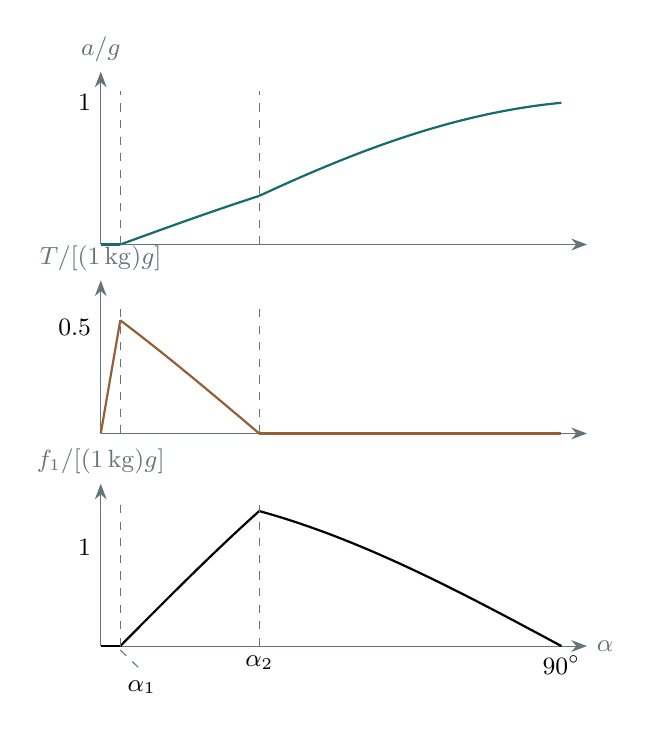
\begin{tikzpicture}[font=\small,x=.065cm]
\begin{scope}[yshift=5.1cm,y=1.8cm]
\draw[axis](0,0)--(95,0);\draw[axis](0,0)--(0,1.22)node[above]{$a/g$};
\draw[traj](0,0)--(3.814074834,0);
\draw[traj,domain=3.814074834:30.963756532,samples=60]plot(\x,{(3*sin(\x)-.2*cos(\x))/4});
\draw[traj,domain=30.963756532:90,samples=80]plot(\x,{sin(\x)-.2*cos(\x)});
\draw[guide](3.814074834,0)--(3.814074834,1.08);\draw[guide](30.963756532,0)--(30.963756532,1.08);
\node[left]at(0,1){$1$};
\end{scope}
\begin{scope}[yshift=2.7cm,y=2.7cm]
\draw[axis](0,0)--(95,0);\draw[axis](0,0)--(0,.72)node[above]{$T/[(1\,\mathrm{kg})g]$};
\draw[thick,color=warm,domain=0:3.814074834,samples=25]plot(\x,{8*sin(\x)});
\draw[thick,color=warm,domain=3.814074834:30.963756532,samples=60]plot(\x,{.6*cos(\x)-sin(\x)});
\draw[thick,color=warm](30.963756532,0)--(90,0);
\draw[guide](3.814074834,0)--(3.814074834,.6);\draw[guide](30.963756532,0)--(30.963756532,.6);
\node[left]at(0,.5){$0.5$};
\end{scope}
\begin{scope}[y=1.25cm]
\draw[axis](0,0)--(95,0)node[right]{$\alpha$};
\draw[axis](0,0)--(0,1.65)node[above]{$f_1/[(1\,\mathrm{kg})g]$};
\draw[thick](0,0)--(3.814074834,0);
\draw[thick,domain=3.814074834:30.963756532,samples=60]plot(\x,{3*sin(\x)-.2*cos(\x)});
\draw[thick,domain=30.963756532:90,samples=80]plot(\x,{1.6*cos(\x)});
\draw[guide](3.814074834,0)--(3.814074834,1.45);\draw[guide](30.963756532,0)--(30.963756532,1.45);
\draw[guide](3.814074834,-.04)--(8,-.25);\node[below]at(8,-.25){$\alpha_1$};
\node[below]at(30.963756532,0){$\alpha_2$};\node[below]at(90,0){$90^\circ$};
\node[left]at(0,1){$1$};
\end{scope}
\end{tikzpicture}
\figcaption{解图 6.10B\quad 三个分区中的加速度、张力与圆柱摩擦分别绘制；竖虚线标出共同分界。}
\end{minipage}\end{center}
拉紧纯滚分支同时取以下三个条件。下滑 $a>0$ 要求 $\tan\alpha>\mu/3$；张力 $T\ge0$ 要求 $\tan\alpha\le3\mu$；纯滚 $f_1\le\mu m_1g\cos\alpha$ 也给 $\tan\alpha\le3\mu$。令
\[
 \alpha_1=\arctan(\mu/3)\approx3.814^\circ,\qquad
 \alpha_2=\arctan(3\mu)\approx30.964^\circ.
\]
当 $0\le\alpha\le\alpha_1$，两者静止。圆柱绕心力矩要求 $f_1=0$，故 $T=m_1g\sin\alpha$；木块静摩擦要承担 $(m_1+m_2)g\sin\alpha$，其上限给上述 $\alpha_1$。

当 $\alpha_1<\alpha\le\alpha_2$，绳拉紧、木块滑动、圆柱纯滚，使用已求通式。$30^\circ$ 位于此区间，先前假设成立。

当 $\alpha>\alpha_2$ 时，按绳只传递拉力的性质取 $T=0$。两物体的平移加速度相同，但圆柱滚滑：
\[
 a=g(\sin\alpha-\mu\cos\alpha),\quad
 f_1=\mu m_1g\cos\alpha,\quad
 r\beta=2\mu g\cos\alpha<a.
\]
$\alpha=90^\circ$ 时 $a=g$，摩擦与张力为零。解图6.10B和下表使用无量纲量 $a/g,r\beta/g$，力另以 $mg$ 的明确质量基准表示。
\begin{center}\small
\begin{tabular}{r|rrrr}
\toprule $\alpha$ & $a/g$ & $f_1/[(1\,\mathrm{kg})g]$ & $T/[(1\,\mathrm{kg})g]$ & $r\beta/g$\\\midrule
$\alpha_1$ &0&0&0.532&0\\
$10^\circ$ &0.081&0.324&0.417&0.081\\
$20^\circ$ &0.210&0.838&0.222&0.210\\
$30^\circ$ &0.332&1.327&0.020&0.332\\
$\alpha_2$ &0.343&1.372&0&0.343\\
$45^\circ$ &0.566&1.131&0&0.283\\
$60^\circ$ &0.766&0.800&0&0.200\\
$75^\circ$ &0.914&0.414&0&0.104\\
$90^\circ$ &1&0&0&0\\\bottomrule
\end{tabular}\end{center}
静止区间的 $T$ 随角度增加；进入滚动区间后 $T$ 逐渐减小到零。$f_1$ 在 $\alpha_2$ 达到峰值，进入滚滑后随 $\cos\alpha$ 减小。
\subsubsection*{下滑时的加速度、张力、摩擦与静止区间}
在解图6.10A的拉紧纯滚分支中，
先由圆柱转动方程和$a=r\beta$得到
$f_1=I_1a/r^2=m_1a/2$。
令$D=3m_1/2+m_2$，两物体平动方程相加，逐项整理为
\[
(m_1+m_2)a=(m_1+m_2)g\sin\alpha
-\mu m_2g\cos\alpha-\frac12m_1a,
\]
\[
a=\frac{[(m_1+m_2)\sin\alpha-\mu m_2\cos\alpha]g}{D}.
\]
再从木块方程取$T=m_2(a-g\sin\alpha+\mu g\cos\alpha)$，
得到
\[
\begin{aligned}
T&=\frac{m_2g}{D}\left[-\frac12m_1\sin\alpha
+\frac32\mu m_1\cos\alpha\right]\\
&=\frac{m_1m_2g(3\mu\cos\alpha-\sin\alpha)}{3m_1+2m_2},
\end{aligned}
\]
\[
f_1=\frac{m_1g[(m_1+m_2)\sin\alpha-\mu m_2\cos\alpha]}{3m_1+2m_2}.
\]
当$a$取沿坡向下为正时，从静止向下起动有$a>0$。绳保持拉紧需要$T\geq0$，圆柱纯滚需要$f_1\leq\mu m_1g\cos\alpha$。静止状态由平衡方程确定，其中木块摩擦取维持平衡所需的静摩擦值。

静止分支中，轴心张力与圆柱重力均不产生绕心力矩，
所以$f_1=0$，圆柱沿坡平衡给$T=m_1g\sin\alpha$。
木块所需静摩擦为
\[
f_2=m_2g\sin\alpha+T=(m_1+m_2)g\sin\alpha,
\]
\[
f_2\leq\mu m_2g\cos\alpha
\quad\Longleftrightarrow\quad
\tan\alpha\leq\frac{\mu m_2}{m_1+m_2}.
\]
等号给出静止区的最大坡角$\alpha_1$。
在拉紧纯滚分支，将$f_1$的通式与上限比较，得到
\[
(m_1+m_2)\sin\alpha
\leq\mu(3m_1+3m_2)\cos\alpha,
\]
故纯滚上限为$\tan\alpha\leq3\mu$。
张力非负也给同一条件。两接触处采用同一摩擦系数且圆柱惯量为$m_1r^2/2$时，张力与静摩擦的临界坡角都由$\mu$决定，质量在比较式中消去。

\subsubsection*{分界连续性、摩擦峰值与零张力}
在$\alpha=\alpha_1$处，纯滚通式给$a=0,f_1=0$，
张力恰等于静止分支的$m_1g\sin\alpha_1$。
在$\alpha=\alpha_2$处，$\sin\alpha_2=3\mu\cos\alpha_2$，
三式给
\[
T=0,\qquad a=2\mu g\cos\alpha_2,\qquad
f_1=\mu m_1g\cos\alpha_2.
\]
这与滚滑分支的极限相同，所以$a,T,f_1$都在分界连续。
解图6.10B分别画三条曲线，静止区的圆柱摩擦保持零，
中段$f_1=m_1a/2$增加，后段$f_1=\mu m_1g\cos\alpha$减小，
故摩擦峰值出现在$\alpha_2$。

对$\alpha>\alpha_2$，零张力解中圆柱与木块的平动方程分别为
\[
m_1a_1=m_1g\sin\alpha-\mu m_1g\cos\alpha,
\qquad
m_2a_2=m_2g\sin\alpha-\mu m_2g\cos\alpha.
\]
所以$a_1=a_2$，而圆柱自旋由
\[
\beta=\frac{f_1r}{I_1}=\frac{2\mu g\cos\alpha}{r},
\qquad a-r\beta=g(\sin\alpha-3\mu\cos\alpha)>0
\]
确定。接触点向下坡滑，取向上坡的动摩擦自洽。
零张力时绳不传递力，几何间距由两物体的相对运动决定：
在本题同系数条件下，两物体若初始速度相同、间距等于绳长，
相同的平动加速度也允许它们保持该间距而绳不受力。
若两处摩擦系数不同，平动加速度不再自动相同，就须重查绳的张紧或松弛状态。

在 $30^\circ$，用两个转变角确定所处运动区间。
$\tan30^\circ=0.577350<0.6=3\mu$且大于$\mu/3$，
所以拉紧纯滚解成立。此时
\[
a=3.25064755\,\mathrm{m/s^2},\quad
\beta=\frac a{0.050\,\mathrm m}=65.0129510\,\mathrm{s^{-2}},
\]
\[
T=0.19222937\,\mathrm N,\quad f_1=13.0025902\,\mathrm N,
\quad \mu N_1=13.5792783\,\mathrm N>f_1.
\]
半径在$a,T,f_1$中约去，但角加速度仍含$1/r$。
下表与解图6.10B的各纵坐标使用明确单位，
加速度除以 $g$，力除以 $(1\,\mathrm{kg})g$，两类量各用自己的单位基准。


\Needspace{18\baselineskip}

\pdfbookmark[2]{第 11 题 逆向自旋乒乓球由滚滑转为纯滚}{q11}

\section*{第 11 题\quad 逆向自旋乒乓球由滚滑转为纯滚}

\tagline{M-06-11}

如图,半径为\(R\)的乒乓球,绕质心轴的转动惯量\(I=\frac{2}{3}mR^{2}\),\(m\)为乒乓球的质量,以一定的初始条件在粗糙的水平面上运动．开始时球的质心速度为
\(v_{\mathrm{C}0}>0\)，向右；初角速度为
\(\omega_0>0\)，逆时针．已知乒乓球与地面之间的摩擦系数为 \(\mu\) .
试求乒乓球开始作纯滚运动所需的时间及纯滚时的质心速度．

\begin{center}\begin{minipage}{\linewidth}\centering
\begin{tikzpicture}[font=\small]
\draw[object](-2,-1)--(3,-1);\draw[object](0,0)circle(1);\draw[motion](0,0)--(1.8,0)node[right]{$v_0$};\draw[motion](.650538239,.650538239)arc(45:250:.92);\node[left]at(-1.2,.5){$\omega_0$ 逆时针};\node[below]at(0,-1){$P$};\node at(.5,-1.9){$I=2mR^2/3$};
\end{tikzpicture}
\figcaption{图 6.11\quad 质心向右、自旋逆时针，最低点起初向右滑。}
\end{minipage}\end{center}

\Needspace{5\baselineskip}\subsection*{解答}

\begin{center}\begin{minipage}{\linewidth}\centering
\begin{tikzpicture}[font=\small]
\draw[object](-2,-1)--(3,-1);\draw[object](0,0)circle(1);\draw[motion](0,0)--(1.8,0)node[right]{$v_0$};\draw[motion](.650538239,.650538239)arc(45:250:.92);\node[left]at(-1.2,.5){$\omega_0$ 逆时针};\node[below]at(0,-1){$P$};\node at(.5,-1.9){$I=2mR^2/3$};\draw[force](0,-1)--(-1.2,-1)node[left]{$f$};\draw[motion](.15,-1.4)--(1.4,-1.4)node[right]{$u=v+R\omega$};
\end{tikzpicture}
\figcaption{解图 6.11A\quad 最低点滑速向右，摩擦向左；逆时针角速度取有符号量。}
\end{minipage}\end{center}
下文简记$v_0=v_{\mathrm C0}$，取向右为平移正向、逆时针为角速度正向。解图6.11A中球的最低接触点 $P$ 的滑速为 $u=v+R\omega$，初值 $u_0=v_0+R\omega_0>0$，摩擦向左。$I=2mR^2/3$，滚滑阶段
\[
 m\dot v=-\mu mg,\qquad I\dot\omega=-\mu mgR.
\]
分别积分并代入初值：
\[
 v=v_0-\mu gt,\qquad \omega=\omega_0-\frac{3\mu g}{2R}t,
 \qquad u=u_0-\frac52\mu gt.
\]
达到 $u=0$ 即为纯滚，注意本题符号约定下是 $v=-R\omega$。于是
\[
 \result{t_1=\frac{2(v_0+R\omega_0)}{5\mu g},\quad
 v_1=\frac35v_0-\frac25R\omega_0,\quad\omega_1=-v_1/R.}
\]
$v_0>2R\omega_0/3$ 时最终向右、顺时针；小于时向左、逆时针；等于时平移与自旋同时停下。平移速度或角速度先过零时，只要接触点的滑速仍满足 $u>0$，滑动摩擦便继续向左。

另一方法取地面固定点 $O$，以顺时针角动量为正。重力与支持力的合力矩相消，摩擦作用线通过地面，外力矩为零，故
\[
 mRv_0-I\omega_0=mRv_1-I\omega_1
 =\left(mR+\frac IR\right)v_1.
\]
这里 $O$ 固定在地面上，当前接触点沿地面移动；摩擦作用线始终通过 $O$，重力和支持力关于 $O$ 的力矩相互抵消。代入惯量得到同一 $v_1$，再由 $t_1=(v_0-v_1)/(\mu g)$ 得时间。$\mu=0$ 且初态不纯滚时，不会达到这终态。
\subsubsection*{两次独立积分与三种到达次序}
初值给$v(0)=v_0>0,\omega(0)=\omega_0>0$。
先把平动与转动方程各自积分，保留积分边界：
\[
\int_{v_0}^{v(t)}\dd v=-\mu g\int_0^t\dd t',
\qquad
\int_{\omega_0}^{\omega(t)}\dd\omega
=-\frac{\mu mgR}{I}\int_0^t\dd t'.
\]
因此$v=v_0-\mu gt$、$\omega=\omega_0-\mu mgRt/I$。
将它们代入有符号纯滚条件$v=-R\omega$，得到
\[
v_0-\mu gt_1=-R\omega_0+\frac{\mu mgR^2}{I}t_1,
\]
\[
t_1=\frac{v_0+R\omega_0}{\mu g(1+mR^2/I)}
=\frac{2(v_0+R\omega_0)}{5\mu g}.
\]
再逐步代回平动速度，
\[
v_1=v_0-\frac25(v_0+R\omega_0)
=\frac35v_0-\frac25R\omega_0.
\]
到达之前$u(t)=v_0+R\omega_0-5\mu gt/2>0$，
故摩擦一直为向左的滑动摩擦；质心反向后，底点仍向右滑到 $t_1$ 才停止。

为明确运动中间发生什么，分别记平移过零时刻和自旋过零时刻为
\[
t_v=\frac{v_0}{\mu g},\qquad
t_\omega=\frac{2R\omega_0}{3\mu g}.
\]
若$v_0>2R\omega_0/3$，则$t_\omega<t_1<t_v$：
自旋先停止后反为顺时针，质心一直向右，最终形成向右的纯滚。
若$v_0<2R\omega_0/3$，则$t_v<t_1<t_\omega$：
质心先停止后向左运动，逆时针自旋尚未停止，最终形成向左的纯滚。
若两者相等，三个时刻相同，平移、自旋、接触滑动同时停止。
这三种情况由同一个滑速函数覆盖，不需要在$v=0$或$\omega=0$处另换摩擦方程。

\subsubsection*{关于固定地面点的角动量与纯滚终速}
解图6.11B把初始地面接触点$O$保留为固定参考点，
而当前接触点记为$P_t$，球心为$C_t$。
球心始终在距地面$R$处，平动角动量的力臂始终为$R$，
与球心水平离开$O$多远无关。
\begin{center}\begin{minipage}{\linewidth}\centering
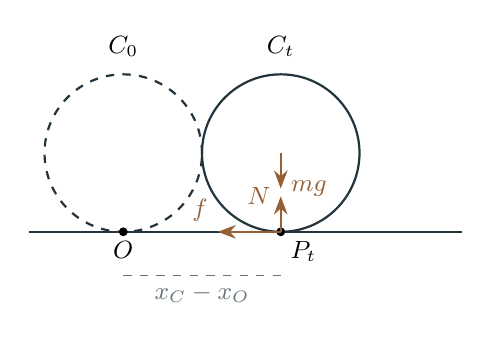
\begin{tikzpicture}
\draw[object](-1.2,0)--(4.3,0);
\draw[object,dashed](0,1)circle(1);\draw[object](2,1)circle(1);
\fill(0,0)circle(1.6pt)node[below]{$O$};
\fill(2,0)circle(1.6pt)node[below right]{$P_t$};
\node[above]at(0,2.1){$C_0$};\node[above]at(2,2.1){$C_t$};
\draw[force](2,0)--(2,.45)node[left]{$N$};
\draw[force](2,1)--(2,.55)node[right]{$mg$};
\draw[force](2,0)--(1.2,0)node[above left]{$f$};
\draw[guide](0,-.55)--(2,-.55)node[midway,below]{$x_C-x_O$};
\end{tikzpicture}
\figcaption{解图6.11B\quad 固定点$O$与当前接触点不同；$N=mg$的两力矩相抵，摩擦作用线通过$O$。}
\end{minipage}\end{center}
关于$O$，重力矩与支持力矩大小均为$(x_C-x_O)mg$、方向相反，
摩擦作用线位于地面，故合外力矩为零。
取顺时针角动量为正，初态与纯滚终态满足
\[
mRv_0-I\omega_0=mRv_1-I\omega_1,
\qquad \omega_1=-v_1/R.
\]
因此
\[
\left(mR+\frac IR\right)v_1=mRv_0-I\omega_0,
\qquad
\left(1+\frac{I}{mR^2}\right)v_1
=v_0-\frac{I}{mR^2}R\omega_0.
\]
代入$I/(mR^2)=2/3$，得$5v_1/3=v_0-2R\omega_0/3$，
得到滑动结束时的纯滚终速。再以$v_1=v_0-\mu gt_1$求时间，便把初、末态的角动量关系接到滑动段的动力学上。
选点后，重力和支持力大小相等、作用线竖直，分别对固定 $O$ 取矩，两项相消。

\subsubsection*{速度图、耗散与转入纯滚}
解图6.11C取$v_0/(R\omega_0)=1/2$，
以$\tau=\mu gt/(R\omega_0)$为横坐标。
质心速度在$\tau=1/2$先过零，
到$\tau_1=3/5$时才有$u=0$，此时$v_1=-R\omega_0/10$，
而$\omega_1=\omega_0/10>0$。
\begin{center}\begin{minipage}{\linewidth}\centering
\begin{tikzpicture}[x=6cm,y=1.6cm]
\draw[axis](0,0)--(.85,0)node[right]{$\tau$};
\draw[axis](0,-.35)--(0,1.8)node[above]{速度$/\,(R\omega_0)$};
\draw[traj](0,.5)--(.6,-.1);\draw[thick,color=warm](0,1)--(.6,.1);
\draw[thick,dashed](0,1.5)--(.6,0);
\draw[guide](.5,-.26)--(.5,.5);\draw[guide](.6,-.26)--(.6,1.35);
\node[below]at(.5,-.26){$1/2$};\node[below]at(.6,-.26){$3/5$};
\node[above]at(.15,1.125){$u$};\node[above left]at(.24,.26){$v$};
\node[above right]at(.48,.28){$R\omega$};
\draw[traj,dashed](.6,-.1)--(.8,-.1);
\draw[thick,color=warm,dashed](.6,.1)--(.8,.1);
\fill(.6,0)circle(.9pt);\node[right]at(.65,.6){$u=0$后不再沿斜率外推};
\end{tikzpicture}
\figcaption{解图6.11C\quad 质心先反向的算例；只有接触滑速过零才结束滚滑，随后无水平外力而匀速纯滚。}
\end{minipage}\end{center}
水平地面无其他阻力时，达到纯滚后不再需要摩擦来改变速度，
可取$f=0$，以$v_1,\omega_1$匀速纯滚；
在 $t_1$ 处，把原来的动摩擦方程接到零摩擦的匀速纯滚方程。
耗散也可用滑速直接积分：
\[
Q=\mu mg\int_0^{t_1}\left(u_0-\frac52\mu gt\right)\dd t
=\frac15m u_0^2>0.
\]
终速不含$\mu$，只是说明达到无滑终态所需总冲量由初态决定；
摩擦仍耗散能量，且时间随$1/\mu$变化。
$\mu=0$ 时滑速始终保持初值 $u_0$，非零初滑速持续存在。


\Needspace{18\baselineskip}

\pdfbookmark[2]{第 12 题 圆柱体滚下斜坡撞墙后的回升高度}{q12}

\section*{第 12 题\quad 圆柱体滚下斜坡撞墙后的回升高度}

\tagline{M-06-12}

如图,实心圆柱体从高度为\(h\)的斜坡上从静止纯滚动地到达水平地面上,继续纯滚动,与光滑竖直墙作完全弹性碰撞后返回,经足够长的水平距离后重新作纯滚动,并纯滚动地爬上斜坡.设地面与圆柱体之间的摩擦系数为\(\mu\),试求圆柱体爬坡所能达到的高度\(h'\).

\begin{center}\begin{minipage}{\linewidth}\centering
\begin{tikzpicture}[font=\small]
\draw[object](-4,3.4)--(-4,0)--(1,0)--(3.55,2.55);
\coordinate(Ci)at(2.730761185,2.65);\coordinate(Cb)at(-1,.65);
\draw[object](Ci)circle(.65);\draw[object](Cb)circle(.65);
\draw[motion](Cb)--(-2.2,.65)node[above]{$v_0$};
\node[above]at(Ci){$v=0$};\node[left]at(-4,2.3){光滑墙};
\draw[guide](Ci)--(4.3,2.65);\draw[guide](1,.65)--(4.3,.65);
\draw[<->](4.05,.65)--(4.05,2.65)node[midway,right]{$h$};
\end{tikzpicture}
\figcaption{图 6.12\quad 高度按质心相对水平段质心的位置量取；光滑墙弹性反弹后返回。}
\end{minipage}\end{center}

\Needspace{5\baselineskip}\subsection*{解答}

\begin{center}\begin{minipage}{\linewidth}\centering
\begin{tikzpicture}[font=\small]
\draw[object](-4,0)--(4,0);
\foreach \x/\ss in {-2.5/{碰前},0/{碰后},2.5/{纯滚}}
{\draw[object](\x,.7)circle(.7);\node at(\x,2){\ss};}
\draw[motion](-2.5,.7)--(-3.7,.7)node[left]{$v_0$};
\draw[motion](0,.7)--(1.2,.7)node[above]{$v_0$};
\draw[motion](2.5,.7)--(2.9,.7)node[right]{$v_0/3$};
\draw[motion](-2.05,1.15)arc(45:250:.636396103);
\draw[motion](.45,1.15)arc(45:250:.636396103);
\draw[motion](2.075735931,1.124264069)arc(135:-70:.6);
\node at(0,-.7){$\omega(0)=v_0/R$逆时针；终态$\omega_1=-v_0/(3R)$};
\end{tikzpicture}
\figcaption{解图 6.12A\quad 解图取离墙为向右；弹性墙碰只反转平移，自旋随后由地面摩擦调整。}
\end{minipage}\end{center}
解图6.12A将过程分成下坡纯滚、光滑墙弹性碰撞、水平滚滑、回坡纯滚。下坡无能量损失，令碰前速率为 $v_0$，有
\[
 mgh=\frac12mv_0^2+\frac12\left(\frac12mR^2\right)\frac{v_0^2}{R^2}
 =\frac34mv_0^2,\qquad v_0=\sqrt{\frac{4gh}{3}}.
\]
墙面冲量通过质心，改变平移方向而不改变角速度。取离墙方向向右为正，碰后 $v(0)=v_0$，逆时针 $\omega(0)=v_0/R$。接触点滑速 $v+R\omega>0$，摩擦向左。滚滑阶段
\[
 v=v_0-\mu gt,\qquad R\omega=v_0-2\mu gt.
\]
纯滚要求 $v=-R\omega$，所以
\[
 t_1=\frac{2v_0}{3\mu g},\qquad v_1=\frac{v_0}{3},\qquad
 \omega_1=-\frac{v_0}{3R}.
\]
随后爬坡纯滚，机械能又守恒：
\[
 mgh'=\frac34mv_1^2=\frac1{12}mv_0^2
 =\frac19mgh,\qquad\result{h'=h/9.}
\]
\begin{center}\begin{minipage}{\linewidth}\centering
\begin{tikzpicture}[font=\small,x=5cm,y=1.8cm]
\draw[axis](0,0)--(.92,0)node[right]{$\tau=\mu gt/v_0$};
\draw[axis](0,-.65)--(0,2.25)node[above]{速度$/v_0$};
\draw[traj](0,1)--(.666666667,.333333333);
\draw[thick,color=warm](0,1)--(.666666667,-.333333333);
\draw[thick,dashed](0,2)--(.666666667,0);
\draw[guide](.5,-.5)--(.5,1.5);\draw[guide](.666666667,-.5)--(.666666667,1.9);
\node[below]at(.5,-.5){$1/2$};\node[below]at(.666666667,-.5){$2/3$};
\node[left]at(0,1){$1$};\node[left]at(0,2){$2$};
\draw[guide](.4,.6)--(.85,.85);\node[right]at(.85,.85){$v/v_0=1-\tau$};
\draw[guide](.4,.2)--(.85,.4);\node[right]at(.85,.4){$R\omega/v_0=1-2\tau$};
\node[above right]at(.18,1.46){$u/v_0=2-3\tau$};
\end{tikzpicture}
\figcaption{解图 6.12B\quad 逆时针角速度先过零，纯滚在有符号速度互为相反数时开始。}
\end{minipage}\end{center}
也可保留摩擦功方法。解图6.12B显示平移速度一直向右，自旋却在 $t=v_0/(2\mu g)$ 反向。摩擦在平移部分的功为
\[
\begin{aligned}
 W_1&=-\mu mg\int_0^{t_1}(v_0-\mu gt)\dd t\\
 &=-\mu mgv_0t_1+\frac12m\mu^2g^2t_1^2
 =-\frac49mv_0^2.
\end{aligned}
\]
对转动的功采用逆时针力矩 $M_C=-\mu mgR$：
\[
\begin{aligned}
 W_2&=-\mu mg\int_0^{t_1}(v_0-2\mu gt)\dd t\\
 &=-\mu mgv_0t_1+m\mu^2g^2t_1^2=-\frac29mv_0^2.
\end{aligned}
\]
转动反向后摩擦矩对转动做正功，但总功仍为负。$W=W_1+W_2=-2mv_0^2/3$，与动能变化
\[
 \frac34m(v_1^2-v_0^2)=-\frac23mv_0^2
\]
一致。因此 $mg(h'-h)=W=-8mgh/9$，再次得到 $h'=h/9$。滚滑距离为 $v_0t_1-\mu gt_1^2/2=4v_0^2/(9\mu g)$；题设的足够长水平段，对应可用质心行程至少达到这个值。
\subsubsection*{墙碰保留动能，水平滑动改变自旋}
图6.12中的$h$与回升的$h'$均按质心相对水平段滚动时质心的高度计。
坡面连接按题设视为无额外碰撞耗能，且坡上静摩擦足以维持纯滚。
对斜角$\alpha$的直坡，实心圆柱的纯滚条件为
$\mu_s\geq\tan\alpha/3$。在这个条件下，坡上静摩擦维持纯滚，两个坡段均可用机械能守恒连接初、末状态。

设$I=mR^2/2$，下坡得到的平动、自转能量分别为
$mv_0^2/2$与$mv_0^2/4$，合为$3mv_0^2/4=mgh$。
墙面光滑，水平冲量通过圆心，关于质心无冲量矩；
完全弹性碰撞将向墙的质心速度反向，大小不变，
逆时针自旋保留原值。因此碰后动能仍为$mgh$，回升高度减少对应随后水平滑动段的能量损失。

碰后$u(0)=2v_0$，而滚滑阶段
\[
\dot u=\dot v+R\dot\omega=-\mu g-2\mu g=-3\mu g.
\]
所以$u=2v_0-3\mu gt$一直为正直至$t_1=2v_0/(3\mu g)$。
自旋在$t_\omega=v_0/(2\mu g)$先过零，
此时质心速度仍为$v_0/2$、接触点仍右滑；
继续受左向动摩擦，才能形成$v_1=v_0/3$、$\omega_1=-v_0/(3R)$。
解图6.12B按实际无量纲纵坐标绘出这三个速度量。
从$t_1$起的能量为
\[
\begin{aligned}
K_1&=\frac12m\left(\frac{v_0}{3}\right)^2
+\frac12\left(\frac12mR^2\right)\left(\frac{v_0}{3R}\right)^2\\
&=\frac1{18}mv_0^2+\frac1{36}mv_0^2
=\frac1{12}mv_0^2=\frac19mgh.
\end{aligned}
\]
随后上坡纯滚，平动、自转一同降到零，故$mgh'=K_1$。

\subsubsection*{摩擦的平动功、转动功及完成纯滚的距离}
把$t_1=2v_0/(3\mu g)$代入平动功的两项，有
\[
W_1=-\frac23mv_0^2+\frac29mv_0^2
=-\frac49mv_0^2.
\]
转动功的两项则给
\[
W_2=-\frac23mv_0^2+\frac49mv_0^2
=-\frac29mv_0^2.
\]
自旋反向后，摩擦矩与角速度同向，转动功率变正。
若以$\tau=\mu gt/v_0$分开积分，便可看清这部分正功：
\[
W_{2,0\to1/2}=-mv_0^2\int_0^{1/2}(1-2\tau)\dd\tau
=-\frac14mv_0^2,
\]
\[
W_{2,1/2\to2/3}=-mv_0^2\int_{1/2}^{2/3}(1-2\tau)\dd\tau
=\frac1{36}mv_0^2.
\]
两段相加仍为$-2mv_0^2/9$，与有符号积分相同。
总摩擦功率则始终满足
\[
P_f=-\mu mg\,v-\mu mgR\omega=-\mu mg\,u\leq0.
\]
因此$W=W_1+W_2=-2mv_0^2/3$，
初、末总动能的差正好等于这段摩擦损失：
\[
K_0-K_1=\frac34m\left(v_0^2-\frac{v_0^2}{9}\right)
=\frac23mv_0^2=-W.
\]
再由$mg(h'-h)=W$，逐步得到
\[
h'-h=-\frac{2v_0^2}{3g}
=-\frac{2}{3g}\frac{4gh}{3}
=-\frac89h,
\qquad h'=\frac19h.
\]
能量法与分功法均把损耗限制在墙碰后的水平滚滑段，前后两段纯滚保留机械能。

要在进入斜坡前恢复纯滚，需要留出下面这段质心水平行程。
从碰后位置到进入坡面前，完成滚滑所需距离为
\[
D_* =\int_0^{t_1}(v_0-\mu gt)\dd t
=\frac{4v_0^2}{9\mu g}=\frac{16h}{27\mu}.
\]
题设足够长就是可用质心水平行程不少于$D_*$。
正$\mu$越小，时间和距离越大；只要仍满足这项长度条件，
终态高度比保持$1/9$。若水平段较短，应把进入坡面时尚未纯滚的
$v,\omega$作为新初值，重新判断摩擦与后续运动。


\Needspace{18\baselineskip}

\pdfbookmark[2]{第 13 题 小球沿圆柱面滚下的无滑条件}{q13}

\section*{第 13 题\quad 小球沿圆柱面滚下的无滑条件}

\tagline{M-06-13}

半径为$r$、质量为$m$的均匀实心小球，从半径为$R$的固定圆柱面顶端自静止滚下。
球心位置角$\varphi$从竖直向上方向量起，静、动摩擦系数均取$\mu$。
\begin{enumerate}
\item 为保证$0\leq\varphi\leq45^\circ$内小球纯滚，求$\mu$的最小值。
\item 取$\mu=0.7$，求纯滚结束时的质心速度$v_1$。
\item 求离开圆柱面的位置角$\varphi_2$满足的方程，不必求解。
\end{enumerate}
运动理解为顶端静止经无穷小偏离后的过程。

\begin{center}\begin{minipage}{\linewidth}\centering
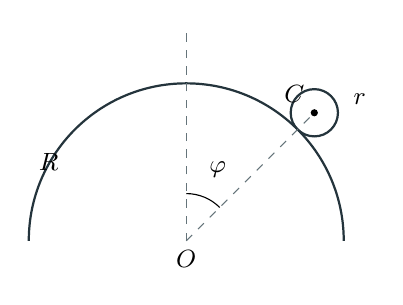
\begin{tikzpicture}[font=\small]
\draw[object](-2,0)arc(180:0:2);
\coordinate(C)at(1.626345597,1.626345597);\coordinate(P)at(1.414213562,1.414213562);
\draw[object](C)circle(.3);\draw[guide](0,0)--(C);
\draw[guide](0,0)--(0,2.7);\draw(0,.6)arc(90:45:.6);
\node at(.4,.9){$\varphi$};\node[below]at(0,0){$O$};
\node[left]at(-1.5,1){$R$};\fill(C)circle(1.3pt);
\node[above left]at(C){$C$};\node[right]at(2,1.8){$r$};
\end{tikzpicture}
\figcaption{图 6.13\quad 小球质心沿半径 $R+r$ 的外侧圆周运动。}
\end{minipage}\end{center}

\Needspace{5\baselineskip}\subsection*{解答}

\begin{center}\begin{minipage}{\linewidth}\centering
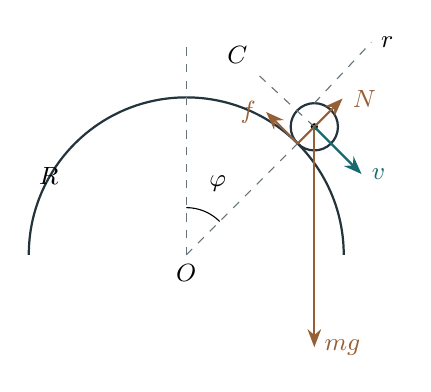
\begin{tikzpicture}[font=\small]
\draw[object](-2,0)arc(180:0:2);
\coordinate(C)at(1.626345597,1.626345597);\coordinate(P)at(1.414213562,1.414213562);
\draw[object](C)circle(.3);\draw[guide](0,0)--(C);
\draw[guide](0,0)--(0,2.7);\draw(0,.6)arc(90:45:.6);
\node at(.4,.9){$\varphi$};\node[below]at(0,0){$O$};
\node[left]at(-1.5,1){$R$};\fill(C)circle(1.3pt);
\draw[force](P)--(1.985786438,1.985786438)node[right]{$N$};
\draw[force](P)--(1.014213562,1.814213562)node[left]{$f$};
\draw[force](C)--++(0,-2.8)node[right]{$mg$};
\draw[motion](C)--++(.6,-.6)node[right]{$v$};
\draw[guide](C)--(.9,2.3);\node[above left]at(.9,2.3){$C$};
\draw[guide](1.626345597,1.926345597)--(2.35,2.7);\node[right]at(2.35,2.7){$r$};
\end{tikzpicture}
\figcaption{解图 6.13A\quad 压力沿外法线，摩擦沿上坡切线；圆心的公转与球的自旋分别计算。}
\end{minipage}\end{center}
设圆柱面半径 $R$、球半径 $r$，质心轨道半径为 $a=R+r$。解图6.13A用 $\varphi$ 表示 $OC$ 相对向上竖直的角；自旋角速度记 $\omega$，轨道角速度为 $\dot\varphi$，二者不同。

纯滚阶段，$v=r\omega=a\dot\varphi$。切向、径向与自旋方程为
\[
 m\dot v=mg\sin\varphi-f,\qquad
 N=mg\cos\varphi-\frac{mv^2}{a},\qquad
 I\dot\omega=fr,\quad I=\frac25mr^2.
\]
消去 $f$ 并用 $v=r\omega$：
\[
 \left(\frac Ir+mr\right)\dot\omega=mg\sin\varphi,
 \quad \dot\omega=\frac{r\omega}{a}\frac{\dd\omega}{\dd\varphi}.
\]
因此 $\omega\dd\omega=[mga/(I+mr^2)]\sin\varphi\dd\varphi$。从零初值积分：
\[
 \frac12\omega^2=\frac{mga}{I+mr^2}(1-\cos\varphi),\qquad
 \omega^2=\frac{10ga}{7r^2}(1-\cos\varphi).
\]
另一方法是能量守恒：$mga(1-\cos\varphi)=(mr^2+I)\omega^2/2$。两个方法得到同一结果。再对角度求导并用 $\dot\varphi=r\omega/a$，有
\[
 \dot\omega=\frac{5g}{7r}\sin\varphi,\quad
 f=\frac27mg\sin\varphi,\quad
 N=\frac{mg}{7}(17\cos\varphi-10).
\]
所以纯滚所需系数为 $q(\varphi)=2\sin\varphi/(17\cos\varphi-10)$。在 $N>0$ 的范围，
\[
 q'(\varphi)=\frac{2(17-10\cos\varphi)}{(17\cos\varphi-10)^2}>0.
\]
要在 $\varphi\le45^\circ$ 内纯滚，最大需求在端点，
\[\result{\mu_{\min}=\frac{2\sin45^\circ}{17\cos45^\circ-10}\approx0.699823.}\]

对题给精确 $\mu=0.7$，纯滚结束角由
\[
 2\sin\varphi_1=0.7(17\cos\varphi_1-10)
\]
确定，数值 $\varphi_1\approx45.00208^\circ$。于是
\[
 \result{v_1=\sqrt{\frac{10}{7}ga(1-\cos\varphi_1)}.}
\]
若近似取 $\varphi_1=45^\circ$，则 $v_1\approx\sqrt{[5(2-\sqrt2)/7]ga}$，它把结束角近似到 $45^\circ$，相应速度也取近似值。

\begin{center}\begin{minipage}{\linewidth}\centering
\begin{tikzpicture}[font=\small,x=4.5cm,y=3cm]
\draw[axis](0,0)--(1.1,0)node[right]{$\varphi/\mathrm{rad}$};
\draw[axis](0,0)--(0,.9)node[above]{力$/\,(mg)$};
\draw[traj,domain=0:.785434498,samples=70]plot(\x,{2*sin(deg(\x))/7});
\draw[thick,color=warm,domain=0:.785434498,samples=70]plot(\x,{.7*(17*cos(deg(\x))-10)/7});
\draw[traj,dashed,domain=.785434498:.941921402,samples=40]plot(\x,{2*sin(deg(\x))/7});
\draw[thick,color=warm,dashed,domain=.785434498:.941921402,samples=40]plot(\x,{.7*(17*cos(deg(\x))-10)/7});
\draw[guide](.785434498,0)--(.785434498,.202037849);
\node[below]at(.785434498,0){$\varphi_1$};
\node[right]at(.35,.63){$\mu N_{\rm roll}/(mg)$};
\node[above]at(.4,.12){$f_{\rm req}/(mg)$};
\end{tikzpicture}
\figcaption{解图 6.13B\quad 所需静摩擦与可供上限在同倍率纵坐标下相交；虚线仅作纯滚延拓。}
\end{minipage}\end{center}
越过解图6.13B的摩擦交点后 $v-r\omega>0$，动摩擦仍向上坡，大小 $\mu N$。改列
\[
 \dot v=g\sin\varphi-\mu N/m,\qquad
 N=mg\cos\varphi-mv^2/a.
\]
设 $y=v^2$，利用 $\dot v=(1/2a)\dd y/\dd\varphi$，消去 $N$ 得
\[
 y'-2\mu y=2ag(\sin\varphi-\mu\cos\varphi).
\]
齐次解为 $Ae^{2\mu\varphi}$；设特解 $B\cos\varphi+C\sin\varphi$，代入并分别比较余弦、正弦系数：
\[
 C-2\mu B=-2\mu ag,\quad -B-2\mu C=2ag,
\]
\[
 B=\frac{2ag(2\mu^2-1)}{1+4\mu^2},\qquad
 C=-\frac{6\mu ag}{1+4\mu^2}.
\]
将速度平方用$ag$归一化，记三角部分为
\[
 D(\varphi)=\frac{2(2\mu^2-1)\cos\varphi-6\mu\sin\varphi}{1+4\mu^2}.
\]
通解 $y=agD(\varphi)+Ae^{2\mu\varphi}$ 用初值 $y(\varphi_1)=v_1^2$ 确定：
\[
 A=[v_1^2-agD(\varphi_1)]e^{-2\mu\varphi_1},
\]
\[
 \frac{v^2}{ag}=D(\varphi)+
 \left[\frac{10}{7}(1-\cos\varphi_1)-D(\varphi_1)\right]
 e^{2\mu(\varphi-\varphi_1)}.
\]
脱离时 $N=0$，即 $v_2^2=ag\cos\varphi_2$。所求方程为
\[
 \result{\cos\varphi_2=D(\varphi_2)+
 \left[\frac{10}{7}(1-\cos\varphi_1)-D(\varphi_1)\right]
 e^{2\mu(\varphi_2-\varphi_1)}.}
\]
应取 $\varphi_2>\varphi_1$ 且途中 $N>0$ 的第一根。滑速在转变处为零；向后增大 $\varphi$，径向压紧减弱，使维持纯滚所需摩擦超出上限，进入该滑动分支。有限摩擦下的脱离角由这段滑动速度与零压力条件共同确定。$\mu=0$ 时 $\varphi_1=0,D=-2\cos\varphi$，方程化为 $\cos\varphi_2=-2\cos\varphi_2+2$，得到光滑极限 $\cos\varphi_2=2/3$。
\subsubsection*{纯滚积分、压力消元及结束速度的全步计算}
球心公转与球的自旋由两条不同的几何长度联系：
$v=a\dot\varphi$使用$a=R+r$，$v=r\omega$使用球半径$r$。
从转动与切向方程消元后，
\[
\left(\frac Ir+mr\right)\dot\omega=mg\sin\varphi,
\qquad
\dot\omega=\frac{r\omega}{a}\frac{\dd\omega}{\dd\varphi},
\]
两式联立，逐项约去$r$给
\[
\omega\dd\omega=\frac{mga}{I+mr^2}\sin\varphi\dd\varphi.
\]
保留积分常量后有
\[
\frac12\omega^2=-\frac{mga}{I+mr^2}\cos\varphi+C_0,
\qquad C_0=\frac{mga}{I+mr^2}.
\]
这里用的是$\varphi=0,\omega=0$的极限初值，
顶点严格静止的解本身不会自行启动，运动理解为任意小偏离后的极限。
代入实心球惯量再乘$r^2$，得到
\[
\omega^2=\frac{10ga}{7r^2}(1-\cos\varphi),
\qquad v^2=\frac{10ga}{7}(1-\cos\varphi).
\]
压力的每一步代入为
\[
\begin{aligned}
N&=mg\cos\varphi-\frac{mr^2}{a}\omega^2\\
&=mg\cos\varphi-\frac{mr^2}{a}\frac{10ga}{7r^2}(1-\cos\varphi)\\
&=mg\left[\cos\varphi-\frac{10}{7}(1-\cos\varphi)\right]
=\frac{mg}{7}(17\cos\varphi-10).
\end{aligned}
\]
求摩擦还可从角速度平方逐级微分，避免把公转角加速度代入自旋转动方程：
\[
2\omega\frac{\dd\omega}{\dd\varphi}
=\frac{10ga}{7r^2}\sin\varphi,
\quad
\frac{\dd\omega}{\dd\varphi}=\frac{5ga}{7r^2\omega}\sin\varphi,
\]
\[
\dot\omega=\frac{r\omega}{a}\frac{5ga}{7r^2\omega}\sin\varphi
=\frac{5g}{7r}\sin\varphi,
\qquad f=\frac Ir\dot\omega=\frac27mg\sin\varphi.
\]
能量法则明确保留平动与自转两项：
\[
mga(1-\cos\varphi)=\frac12mv^2+\frac12I\omega^2
=\frac12(mr^2+I)\omega^2.
\]
能量式给出与动力学积分相同的速度。静摩擦对球心有力矩，提供自转角加速度。纯滚时受力点相对圆柱瞬时静止，摩擦功率为零。

在 $\varphi_1$ 处，压力与结束速度通过径向方程联系：
\[
N_1=\frac{mg}{7}(17\cos\varphi_1-10),
\]
\[
\frac{v_1^2}{a}=g\cos\varphi_1-\frac{N_1}{m}
=g\cos\varphi_1-\frac g7(17\cos\varphi_1-10)
=\frac{10g}{7}(1-\cos\varphi_1).
\]
精确$\mu=0.7$给$\varphi_1=0.7854344984\,\mathrm{rad}$，
$v_1/\sqrt{ga}=0.6468814332$。
解图6.13B比较的是同倍率的$f$与$\mu N$，交点才对应摩擦刚取满；
交点后的虚线延续纯滚表达式，实际受力从此按滑动分支求出。

\subsubsection*{滚滑一阶方程的系数、常量与初值}
令$y=v^2$。沿球心轨道的链式法则逐步给出
\[
\dot v=\frac{\dd v}{\dd\varphi}\dot\varphi
=\frac va\frac{\dd v}{\dd\varphi}
=\frac1{2a}\frac{\dd y}{\dd\varphi}.
\]
将$f=\mu N$代入切向方程，再用径向方程消元：
\[
mg\sin\varphi-\mu N=\frac{m}{2a}y',
\qquad N=mg\cos\varphi-\frac{my}{a},
\]
\[
\frac1{2a}y'=g\sin\varphi-\mu g\cos\varphi+\frac\mu a y.
\]
乘$2a$并移项才得到$y'-2\mu y=2ag(\sin\varphi-\mu\cos\varphi)$。
方程的系数在 $\mu=0$ 处仍有限，可以连续取光滑极限。

齐次部分满足$y_h'-2\mu y_h=0$，积分为$y_h=Ae^{2\mu\varphi}$。
非齐次特解取$y_p=B\cos\varphi+C\sin\varphi$，逐项代入：
\[
-B\sin\varphi+C\cos\varphi-2\mu(B\cos\varphi+C\sin\varphi)
=2ag\sin\varphi-2\mu ag\cos\varphi.
\]
由于该式应对区间内所有角度成立，须分别比较两种三角函数的系数：
\[
-B-2\mu C=2ag,\qquad C-2\mu B=-2\mu ag.
\]
先用$B=-2\mu C-2ag$消元，得到
$C(1+4\mu^2)=-6\mu ag$，再代回即恢复前面的$B,C$。
指数项保留初态影响，三角特解给出重力和动摩擦持续作用的部分。

将$y(\varphi_1)=v_1^2$代入，积分常量的展开式为
\[
\begin{aligned}
A=\frac{ag}{1+4\mu^2}\Bigl[&\frac{10}{7}(1+4\mu^2)(1-\cos\varphi_1)\\
&-2(2\mu^2-1)\cos\varphi_1+6\mu\sin\varphi_1\Bigr]
e^{-2\mu\varphi_1}.
\end{aligned}
\]
分母$1+4\mu^2$作用于整个中括号，
再乘 $e^{2\mu\varphi}$，指数因子合成 $e^{2\mu(\varphi-\varphi_1)}$。
在$\varphi=\varphi_1$代回通解，三角项抵消后应恰剩$v_1^2$，
从而接上滑动开始时的同一个速度。

记中括号为$K$，则脱离条件也可把前面的方程整理为
\[
3\cos\varphi_2+6\mu\sin\varphi_2
=K e^{2\mu(\varphi_2-\varphi_1)},
\]
\[
K=\frac{10}{7}(1+4\mu^2)(1-\cos\varphi_1)
-2(2\mu^2-1)\cos\varphi_1+6\mu\sin\varphi_1.
\]
这里$\varphi_1$由纯滚结束条件确定，$\mu=0.7$用于整个滚滑方程。
解图6.13C把$z=v^2/(ag)$与$\cos\varphi$作比较；
两者的第一次相交使$N/(mg)=\cos\varphi-z$归零。
\begin{center}\begin{minipage}{\linewidth}\centering
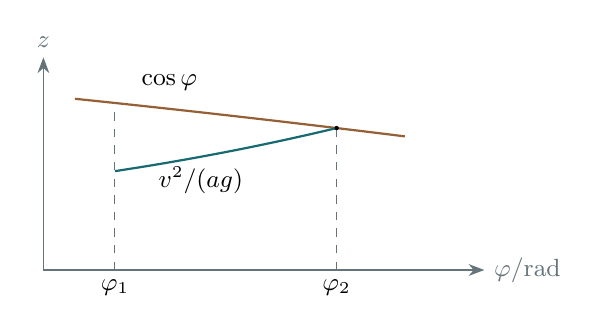
\begin{tikzpicture}[x=20cm,y=3cm,font=\small]
\draw[axis](.74,0)--(1.02,0)node[right]{$\varphi/\mathrm{rad}$};
\draw[axis](.74,0)--(.74,.9)node[above]{$z$};
\draw[thick,color=warm,domain=.76:.97,samples=70]plot(\x,{cos(deg(\x))});
\draw[traj,domain=.785434498:.926210503,samples=90]plot(\x,{-.013513513514*cos(deg(\x))-1.418918918919*sin(deg(\x))+1.431374383220*exp(1.4*(\x-.785434498423))});
\draw[guide](.785434498,0)--(.785434498,.707081088);
\draw[guide](.926210503,0)--(.926210503,.600867419);
\node[below]at(.785434498,0){$\varphi_1$};\node[below]at(.926210503,0){$\varphi_2$};
\node[above]at(.82,.72){$\cos\varphi$};\node[below]at(.84,.48){$v^2/(ag)$};
\fill(.926210503,.600867419)circle(.8pt);
\end{tikzpicture}
\figcaption{解图6.13C\quad $\mu=0.7$的滑动分支；从$\varphi_1$起找首次零压力，不延用纯滚速度。}
\end{minipage}\end{center}

\subsubsection*{向上坡动摩擦是否始终自洽}
设$u=v-r\omega$为接触滑速，$n=N/(mg)=\cos\varphi-z$。
滑动分支的平动、自旋分别给
\[
\frac{\dot u}{g}=\sin\varphi-\frac72\mu n=:H(\varphi),
\qquad n'=-3\sin\varphi+2\mu n.
\]
在转变点$f=\mu N$，有$H(\varphi_1)=0,u(\varphi_1)=0$。
消去$n$后，
\[
H'-2\mu H=\cos\varphi+\frac{17}{2}\mu\sin\varphi>0
\qquad(\varphi_1<\varphi<\pi/2).
\]
乘积分因子$e^{-2\mu\varphi}$并从$\varphi_1$积分，得$H>0$，
于是$\dot u>0,u>0$，向上坡的动摩擦方向在这一段始终自洽。
同时
\[
n'=-\frac{17}{7}\sin\varphi-\frac47H<0,
\]
压力持续减小，在第一个零点结束接触。
这一段采用滑动速度求压力，离面角取滑动压力的零点。
$\mu=0$时初态无自旋加速，方程退为质点在半径$a$轨道上的滑动，
给$\cos\varphi_2=2/3$，与直接使用能量和零压力条件一致。
\subsubsection*{用积分因子求下滑速度}
同一线性方程乘以$e^{-2\mu\varphi}$，有
\[
\frac{\dd}{\dd\varphi}\left(ye^{-2\mu\varphi}\right)
=2ag e^{-2\mu\varphi}(\sin\varphi-\mu\cos\varphi).
\]
在结束角$\varphi_1$处取$y(\varphi_1)=v_1^2$，积分得到
\[
y(\varphi)=v_1^2 e^{2\mu(\varphi-\varphi_1)}
+2ag e^{2\mu\varphi}\int_{\varphi_1}^{\varphi}
e^{-2\mu\psi}(\sin\psi-\mu\cos\psi)\dd\psi.
\]
积分中的一个原函数为
\[
\frac{e^{-2\mu\psi}}{1+4\mu^2}
[(2\mu^2-1)\cos\psi-3\mu\sin\psi].
\]
原函数的分母为$1+4\mu^2$。上限给出三角特解，下限连同初值项给出随角差变化的指数项；当$\varphi=\varphi_1$时，积分为零，速度连续接上$v_1$。式中各项在$\mu=0$处连续，光滑轨道的结果可直接取$\mu\to0$得到。



\Needspace{18\baselineskip}

\pdfbookmark[2]{第 14 题 两相同实心球弹性碰撞后的滚动}{q14}

\section*{第 14 题\quad 两相同实心球弹性碰撞后的滚动}

\tagline{M-06-14}

在水平地面上有两个完全相同的均匀实心球,其一作纯滚动,质心速度为\(v\),另一静止不动.两球作完全弹性碰撞,因碰撞时间很短,碰撞过程中摩擦力的影响可以忽略不计.

试求:1. 碰后两球达到纯滚时的质心速度. 2. 全部过程中损失的机械能的百分数.

两球沿连心线正碰，球间无切向冲量；地面粗糙，碰后有充分时间达到纯滚。

\begin{center}\begin{minipage}{\linewidth}\centering
\begin{tikzpicture}[font=\small]
\draw[object](-2,-.7)--(4,-.7);\foreach \x/\s in {0/1,2.4/2}{\draw[object](\x,0)circle(.7);\node at(\x,.1){球\s};}\draw[motion](0,.95)--(1.5,.95)node[right]{$v$};\draw[motion](-.494974747,.494974747)arc(135:-100:.7);\node[below]at(2.4,-1){静止};
\end{tikzpicture}
\figcaption{图 6.14\quad 球1纯滚，沿连心线正碰静止球2。}
\end{minipage}\end{center}

\Needspace{5\baselineskip}\subsection*{解答}

\begin{center}\begin{minipage}{\linewidth}\centering
\begin{tikzpicture}[font=\small]
\foreach \y/\lab in {2/{碰前},0/{刚碰后},-2/{滚滑}}{\draw[object](-1,\y-.6)--(4,\y-.6);\foreach \x/\i in {0/1,2.5/2}{\draw[object](\x,\y)circle(.6);\node at(\x,\y){\i};}\node[left]at(-1,\y){\lab};}\draw[motion](0,2.9)--(1.1,2.9)node[right]{$v$};\draw[motion](2.5,.9)--(3.6,.9)node[right]{$v$};\draw[force](0,-2.6)--(1,-2.6)node[below]{$f_1$};\draw[force](2.5,-2.6)--(1.5,-2.6)node[below]{$f_2$};\node[right]at(4,0){$R\omega_1'=v,\ \omega_2'=0$};
\end{tikzpicture}
\figcaption{解图 6.14A\quad 刚碰后球1有自旋、球2有平移，底点滑速相反。}
\end{minipage}\end{center}
解图6.14A列出碰前、刚碰后与滚滑三阶段。取向右、顺时针为正。碰撞为沿连心线的正碰，两球质量相同、法向完全弹性，球间无切向冲量，故质心速度交换，自旋不变：
\[
 v_1'=0,\quad R\omega_1'=v,\qquad
 v_2'=v,\quad R\omega_2'=0.
\]
球1接触点滑速 $v_1'-R\omega_1'=-v$，摩擦向右；球2滑速为 $v$，摩擦向左。

先用地面固定点的角动量守恒。重力与支持力矩相消，摩擦力矩为零。令 $I=2mR^2/5$，各球纯滚时 $\omega_i''=v_i''/R$，
\[
 \left(mR+\frac IR\right)v_1''=I\frac vR,
 \qquad
 \left(mR+\frac IR\right)v_2''=mRv.
\]
所以 $v_1''=2v/7$、$v_2''=5v/7$。

\begin{center}\begin{minipage}{\linewidth}\centering
\begin{tikzpicture}[font=\small,x=14cm,y=3cm]
\draw[axis](0,0)--(.36,0)node[right]{$\tau=\mu gt/v$};
\draw[axis](0,0)--(0,1.15)node[above]{速度$/v$};
\draw[traj](0,0)--(.285714286,.285714286);
\draw[thick,color=warm](0,1)--(.285714286,.714285714);
\draw[guide](.285714286,0)--(.285714286,1.03);
\node[below]at(.285714286,0){$2/7$};\node[left]at(0,1){$1$};
\node[right]at(.3,.285714286){$v_1/v=2/7$};
\node[right]at(.3,.714285714){$v_2/v=5/7$};
\end{tikzpicture}
\figcaption{解图 6.14B\quad 两球同一时刻达到纯滚，前球始终更快而继续分离。}
\end{minipage}\end{center}
动力学方法保留每球的摩擦阶段。解图6.14B中球1满足
\[
 v_1(t)=\mu gt,\qquad R\omega_1(t)=v-\frac52\mu gt;
\]
球2满足
\[
 v_2(t)=v-\mu gt,\qquad R\omega_2(t)=\frac52\mu gt.
\]
分别令 $v_i=R\omega_i$，两者恰在同一时刻 $t_*=2v/(7\mu g)$ 达到纯滚，代回得到
\[\result{v_1''=\frac27v,\qquad v_2''=\frac57v.}\]
两球碰后分离，球2始终比球1快，不发生再次相撞。初始总动能和最终总动能分别为
\[
 E_0=\frac12mv^2+\frac12I(v/R)^2=\frac7{10}mv^2,
\]
\[
 E_f=\frac7{10}m\left[\left(\frac{2v}{7}\right)^2+
 \left(\frac{5v}{7}\right)^2\right]=\frac{29}{49}E_0.
\]
因此损失比例为
\[\result{\frac{E_0-E_f}{E_0}=\frac{20}{49}\approx40.816\%.}\]
能量在碰撞瞬间守恒，损失发生在两球随后与地面的滑动摩擦过程。
\subsubsection*{两球的角动量分别列式}
仍取顺时针为角速度正向。
关于地面固定点，重力与支持力的矩相抵、地面摩擦的矩为零，
所以每个球在碰后滚滑段各自守恒$mRv+I\omega$。
球1刚碰后只有自旋，球2刚碰后只有平移，故
\[
L_1'=I\frac vR,\qquad L_2'=mRv.
\]
纯滚终态分别有
\[
L_1''=\left(\frac IR+mR\right)v_1'',
\qquad
L_2''=\left(\frac IR+mR\right)v_2''.
\]
分别将每个球的初末角动量相等，得到两球各自的纯滚终速：
\[
v_1''=\frac{I}{I+mR^2}v=\frac{2/5}{1+2/5}v=\frac27v,
\]
\[
v_2''=\frac{mR^2}{I+mR^2}v=\frac{1}{1+2/5}v=\frac57v.
\]
碰撞使平移速度交换，自旋仍分别留在碰前的球上。

\subsubsection*{动力学积分、相同结束时间与分离条件}
球1的底点起初向左滑，地面动摩擦向右；
其平动、自旋方程与初值为
\[
\dot v_1=\mu g,\quad \dot\omega_1=-\frac{\mu mgR}{I},
\qquad v_1(0)=0,\quad\omega_1(0)=v/R.
\]
积分后$v_1=\mu gt$、$\omega_1=v/R-\mu mgRt/I$，
纯滚给
\[
\mu gt_1=v-\frac{\mu mgR^2}{I}t_1,
\qquad t_1=\frac{v}{\mu g(1+mR^2/I)}=\frac{2v}{7\mu g}.
\]
球2的底点起初向右滑，摩擦向左；独立列出
\[
\dot v_2=-\mu g,\quad \dot\omega_2=\frac{\mu mgR}{I},
\qquad v_2(0)=v,\quad\omega_2(0)=0,
\]
得到$v_2=v-\mu gt$、$\omega_2=\mu mgRt/I$，从而
\[
v-\mu gt_2=\frac{\mu mgR^2}{I}t_2,
\qquad t_2=\frac{2v}{7\mu g}=t_1.
\]
两球同时结束滚滑，是因为初始底点滑速大小相同，
而同一惯量和摩擦系数使其变化率大小也相同。
在$0\leq t\leq t_*$内，前球与后球的质心速度差为
\[
v_2-v_1=v-2\mu gt\geq\frac37v>0.
\]
若从刚分离的接触位置计，间隙增长量为
\[
\Delta d(t)=\int_0^t(v-2\mu gt')\dd t'=vt-\mu gt^2>0.
\]
所以两个独立的地面滚滑过程相容，没有在到达纯滚前再次碰撞。
之后前球仍以$5v/7$快于后球的$2v/7$，继续分离。

\subsubsection*{碰撞守恒与地面耗散的能量分项}
初始能量只有球1贡献，平动、自转分别为$mv^2/2,mv^2/5$。
刚碰后平动能转到球2，自转能仍在球1，总能量仍是$7mv^2/10$。
最终四项动能应分别平方后相加：
\[
\begin{aligned}
K_{1f}&=\frac12m\left(\frac{2v}{7}\right)^2
+\frac15m\left(\frac{2v}{7}\right)^2=\frac2{35}mv^2,\\
K_{2f}&=\frac12m\left(\frac{5v}{7}\right)^2
+\frac15m\left(\frac{5v}{7}\right)^2=\frac5{14}mv^2,\\
K_f&=\frac{29}{70}mv^2.
\end{aligned}
\]
球1从自转能$mv^2/5$变到$2mv^2/35$，损失$mv^2/7$；
球2从平动能$mv^2/2$变到$5mv^2/14$，也损失$mv^2/7$。
因此
\[
\Delta E=\frac27mv^2,\qquad
\frac{\Delta E}{E_0}
=\frac{(2/7)mv^2}{(7/10)mv^2}=\frac{20}{49}
=40.8163265\ldots\%.
\]
每球底点的相对滑程还给出同一耗散量：
$u_1=-v+7\mu gt/2$、$u_2=v-7\mu gt/2$，
其绝对值相等，所以
\[
Q_1=Q_2=\mu mg\int_0^{t_*}\left(v-\frac72\mu gt\right)\dd t
=\frac17mv^2.
\]
两地面摩擦冲量大小相等、方向相反，故总平移动量仍为$mv$；
但两接触处均有相对滑动，总机械能并不守恒。
碰撞瞬间守恒能量；之后到$t_*$为止，两处滑动共产生$2mv^2/7$的热量。
解图6.14C补画最后的纯滚状态。球2仍在前且速度较大，
两球均顺时针转动；无其他水平外力时不再需要静摩擦来改变运动，
从此各自以零摩擦匀速纯滚。
\begin{center}\begin{minipage}{\linewidth}\centering
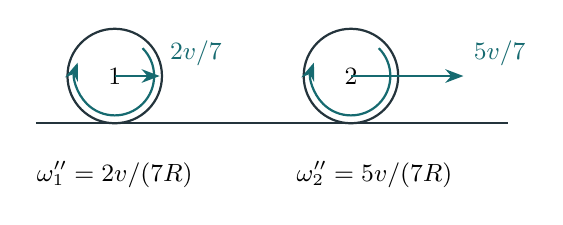
\begin{tikzpicture}
\draw[object](-1,0)--(5,0);
\foreach \xx/\ii in {0/1,3/2}{\draw[object](\xx,.6)circle(.6);\node at(\xx,.6){\ii};}
\draw[motion](0,.6)--(.571428571,.6)node[above right]{$2v/7$};
\draw[motion](3,.6)--(4.428571429,.6)node[above right]{$5v/7$};
\draw[motion](.353553391,.953553391)arc(45:-200:.5);
\draw[motion](3.353553391,.953553391)arc(45:-200:.5);
\node at(0,-.65){$\omega_1''=2v/(7R)$};
\node at(3.3,-.65){$\omega_2''=5v/(7R)$};
\end{tikzpicture}
\figcaption{解图6.14C\quad 两球最终均向右纯滚，前球较快而继续分离；箭头按同一平动速度比例绘制。}
\end{minipage}\end{center}



\Needspace{18\baselineskip}

\pdfbookmark[2]{第 15 题 两圆柱轮与轻杆连接系统的运动}{q15}

\section*{第 15 题\quad 两圆柱轮与轻杆连接系统的运动}

\tagline{M-06-15}

如图,两个质量和半径均相同的实心圆柱轮,它们的质心轴互相平行,并用一轻杆相

连,轴与轴承间的摩擦忽略不计. 两轮先以共同的初速 \(v_{0}\)
沿水平方向运动,两轮的初角速度为零(如上图).
然后同时轻轻与地面相接触(如下图). 设两轮与地面之间的摩擦系数分别为
\(\mu_{1}\) 和 \(\mu_{2}(\mu_{1}>\mu_{2})\).
试求两轮均变为纯滚动所需的时间及纯滚后的平动速度.

\begin{center}\begin{minipage}{\linewidth}\centering
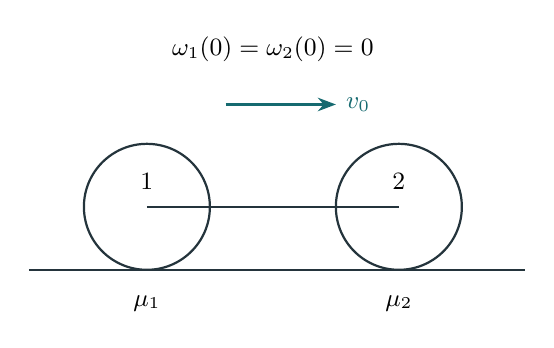
\begin{tikzpicture}[font=\small]
\draw[object](-1.5,-.8)--(4.8,-.8);\foreach \x/\i in {0/1,3.2/2}{\draw[object](\x,0)circle(.8);\node[above]at(\x,.1){\i};\node[below]at(\x,-1){$\mu_\i$};}\draw[object](0,0)--(3.2,0);\draw[motion](1,1.3)--(2.4,1.3)node[right]{$v_0$};\node at(1.6,2){$\omega_1(0)=\omega_2(0)=0$};
\end{tikzpicture}
\figcaption{图 6.15\quad 轻杆连接轴心；两轮角速度可以不同。}
\end{minipage}\end{center}

\Needspace{5\baselineskip}\subsection*{解答}

\begin{center}\begin{minipage}{\linewidth}\centering
\begin{tikzpicture}[font=\small]
\draw[object](-2,0)--(5,0);
\foreach \xx/\ii in {0/1,3.2/2}{\draw[object](\xx,.8)circle(.8);\node[above]at(\xx,1){\ii};}
\draw[object](0,.8)--(3.2,.8);
\draw[force](0,0)--(-1.5,0)node[midway,below]{$\mu_1mg$};
\draw[force](3.2,0)--(2.7,0)node[midway,below]{$\mu_2mg$};
\draw[force](0,.8)--(.5,.8)node[above]{$H$};
\draw[force](3.2,.8)--(2.7,.8)node[above]{$H$};
\draw[motion](1,2.1)--(2.2,2.1)node[right]{$v$};
\node at(1.6,2.7){两轮均滑；示例$\mu_1=3\mu_2$，杆受拉};
\end{tikzpicture}
\figcaption{解图 6.15A\quad 第一阶段两轮都滑，摩擦均向后；轻杆只约束轴心间距。}
\end{minipage}\end{center}
两轮各质量 $m$、惯量 $I=mR^2/2$，轻杆只传递轴心处水平力，不限制两轮自旋角速度相等。解图6.15A取向右、顺时针为正，$\mu_1>\mu_2>0$。

第一阶段两轮都向前滑，摩擦均向左。整体平移与分别绕心转动给
\[
 2ma=-(\mu_1+\mu_2)mg,\qquad I\beta_i=\mu_i mgR.
\]
积分得
\[
 v=v_0-\frac12(\mu_1+\mu_2)gt,\qquad
 R\omega_i=2\mu_i gt.
\]
轮1先达到 $v=R\omega_1$，因此
\[
 t_1=\frac{2v_0}{(5\mu_1+\mu_2)g},\qquad
 v(t_1)=\frac{4\mu_1}{5\mu_1+\mu_2}v_0.
\]

\begin{center}\begin{minipage}{\linewidth}\centering
\begin{tikzpicture}[font=\small]
\draw[object](-2,0)--(5,0);
\foreach \xx/\ii in {0/1,3.2/2}{\draw[object](\xx,.8)circle(.8);\node[above]at(\xx,1){\ii};}
\draw[object](0,.8)--(3.2,.8);
\draw[force](0,0)--(.3,0)node[midway,below]{$\mu_2mg/5$};
\draw[force](3.2,0)--(1.7,0)node[midway,below]{$\mu_2mg$};
\draw[force](0,.8)--(-.9,.8)node[above]{$-H$};
\draw[force](3.2,.8)--(4.1,.8)node[above]{$-H$};
\node at(1.6,2.2){轮1纯滚，轮2仍滑；杆受压};
\end{tikzpicture}
\figcaption{解图 6.15B\quad 轮1静摩擦反向为向右，保证共同减速时角速度同步降低。}
\end{minipage}\end{center}
第二阶段轮1纯滚、轮2仍滑。解图6.15B的轮1静摩擦实际向右。先仍把向左摩擦记为有符号的 $f_1$，有
\[
 2ma=-f_1-\mu_2mg,\quad I\beta_1=f_1R,\quad a=R\beta_1.
\]
由 $f_1=ma/2$ 得 $a=-2\mu_2g/5$、$f_1=-\mu_2mg/5$。所需向右静摩擦小于轮1上限 $\mu_1mg$，因此该阶段成立。

令 $v=-2\mu_2gt/5+C_0$，在 $t_1$ 连续接上初值，
\[
 C_0=v(t_1)+\frac25\mu_2gt_1
 =\frac{4\mu_1+4\mu_2/5}{5\mu_1+\mu_2}v_0=\frac45v_0.
\]
轮2仍有 $R\omega_2=2\mu_2gt$。在 $t_2$ 两轮全纯滚，
\[
 \frac45v_0-\frac25\mu_2gt_2=2\mu_2gt_2,
 \quad\result{t_2=\frac{v_0}{3\mu_2g},\qquad v_f=\frac23v_0.}
\]
第三阶段无外部水平力，二轮匀速纯滚，$\omega_1=\omega_2=2v_0/(3R)$。

另一方法取地面固定点，整体角动量守恒，
\[
 2mRv_0=2mRv_f+2I\omega_f,
 \qquad v_f=R\omega_f.
\]
由此直接得到 $v_f=2v_0/3$。轮2一直滑至终态，角加速度 $2\mu_2g/R$ 恒定，所以 $t_2=\omega_f/\beta_2=v_0/(3\mu_2g)$。$\mu_1=\mu_2$ 时 $t_1=t_2$，中间阶段消失；$\mu_2=0$ 时轮2始终保持零自旋，只有轮1在后续进入纯滚。
\subsubsection*{共同平移、不同自旋与第一转变时刻}
轻杆连接的是轴心，两个轮半径相同且都接地，
轴心等高使杆保持水平，只传递水平轴力，因此各轮$N_i=mg$。
无摩擦轴承允许轮子自由自旋。水平轻杆通过轴承传递轴向力，作用线通过轮心。
令$H$表示杆对轮1向右的有符号作用力，杆对轮2为$-H$。
在两轮都滑的第一阶段，分别列出两轮平动方程：
\[
ma=H-\mu_1mg,\qquad ma=-H-\mu_2mg.
\]
相加得到共同加速度，相减得到杆力，
\[
a=-\frac{\mu_1+\mu_2}{2}g,
\qquad H=\frac{\mu_1-\mu_2}{2}mg>0.
\]
此时杆受拉，轮1受到向前牵引、轮2受到向后牵引。
两轮的摩擦矩分别给
\[
\beta_1=\frac{\mu_1mgR}{mR^2/2}=\frac{2\mu_1g}{R},
\qquad
\beta_2=\frac{2\mu_2g}{R}.
\]
两轮的自旋积分均取初值 $\omega_i(0)=0$。
底点滑速分别为
\[
u_1=v-R\omega_1=v_0-\frac{5\mu_1+\mu_2}{2}gt,
\quad
u_2=v-R\omega_2=v_0-\frac{\mu_1+5\mu_2}{2}gt.
\]
$\mu_1>\mu_2$使$u_1$下降得更快。
在$t_1$第一次归零时，轮2仍有
\[
u_2(t_1)=\frac{4(\mu_1-\mu_2)}{5\mu_1+\mu_2}v_0>0.
\]
第一轮在此刻纯滚，第二轮的正滑速仍对应向后的动摩擦。

\subsubsection*{第二阶段的静摩擦、杆力及连续初值}
轮1纯滚以后，$f_1$ 由无滑约束与动力学方程共同确定。
以向左为正记$f_1$，从$2ma=-f_1-\mu_2mg$及
$f_1R=I\beta_1,\ a=R\beta_1$联立，逐步得到
\[
f_1=\frac{I}{R^2}a=\frac12ma,
\qquad \frac52ma=-\mu_2mg,
\]
\[
a=-\frac25\mu_2g,\qquad f_1=-\frac15\mu_2mg.
\]
负号表示轮1静摩擦实际向右，以使减速的轮1同步减小顺时针自旋。
其大小$\mu_2mg/5<\mu_1mg$，满足静摩擦约束。
解图6.15B的两箭头大小比为$1:5$。
再从轮1的平动方程求杆力，有
\[
ma=H+\frac15\mu_2mg,
\qquad H=-\frac35\mu_2mg<0.
\]
杆由受拉变为受压，对轮1向后推、对轮2向前推。
这项转换依赖轻杆可承压；若改成只能拉的轻绳，第二阶段须重新分析。

以同一个触地时刻为$t=0$，第二阶段速度先写为
$v=-2\mu_2gt/5+C_0$。
利用$t=t_1$时速度连续，积分常量的逐项代入为
\[
\begin{aligned}
C_0&=v(t_1)+\frac25\mu_2gt_1\\
&=\frac{4\mu_1}{5\mu_1+\mu_2}v_0
+\frac25\mu_2g\frac{2v_0}{(5\mu_1+\mu_2)g}\\
&=\frac{4\mu_1+4\mu_2/5}{5\mu_1+\mu_2}v_0=\frac45v_0.
\end{aligned}
\]
若改用从$t_1$起算的新时间，速度初值须改写为$v(t_1)$，
积分常量随时间原点一同转换。
轮2直到结束仍按同一恒角加速度增加自旋，
故$v=4v_0/5-2\mu_2gt/5$与$R\omega_2=2\mu_2gt$相交给$t_2$。
第二阶段持续时间为
\[
t_2-t_1=\frac{5(\mu_1-\mu_2)v_0}{3\mu_2(5\mu_1+\mu_2)g}>0,
\]
\[
u_2(t)=\frac45v_0-\frac{12}{5}\mu_2gt
=\frac{12}{5}\mu_2g(t_2-t)>0\quad(t_1\leq t<t_2).
\]
所以轮2在该阶段持续向前滑，不需中途再次改变摩擦方向。

\begin{center}\begin{minipage}{\linewidth}\centering
\begin{tikzpicture}[x=10cm,y=3cm,font=\small]
\draw[axis](0,0)--(.43,0)node[right]{$\tau=\mu_2gt/v_0$};
\draw[axis](0,0)--(0,1.2)node[above]{速度$/v_0$};
\draw[traj](0,1)--(.125,.75)--(.333333333,.666666667);
\draw[thick,color=warm,dashed](0,0)--(.125,.75)--(.333333333,.666666667);
\draw[thick,dash dot](0,0)--(.333333333,.666666667);
\draw[guide](.125,0)--(.125,1.08);\draw[guide](.333333333,0)--(.333333333,1.08);
\node[below]at(.125,0){$t_1$};\node[below]at(.333333333,0){$t_2$};
\node[left]at(0,1){$1$};\node[above]at(.24,.704){$v=R\omega_1$};
\node[above left]at(.07,.42){$R\omega_1$};\node[below right]at(.18,.36){$R\omega_2$};
\draw[traj](.333333333,.666666667)--(.41,.666666667);
\end{tikzpicture}
\figcaption{解图6.15C\quad 取$\mu_1=3\mu_2$；共同速度先后与两条自旋速度相遇，第二阶段轮1始终纯滚。}
\end{minipage}\end{center}

\subsubsection*{共同纯滚后的终速、耗散与零摩擦情形}
两轮都纯滚后，令各自向左摩擦为$f_i$。
由$\beta_i=a/R$及$I\beta_i=f_iR$，有$f_1=f_2=ma/2$。
整体方程$2ma=-f_1-f_2=-ma$给$a=0$，
所以两摩擦与杆力都归零，此后保持匀速纯滚。

在运动平面内选地面上的固定点，两个摩擦的作用线均过该点，力矩为零；
各轮重力与支持力的矩相消，杆的内部力矩在系统内相消。
因此系统角动量守恒，初态与终态逐项为
\[
L_0=2mRv_0,
\qquad
L_f=2mRv_f+I\omega_{1f}+I\omega_{2f}
=2mRv_f+2I\frac{v_f}{R}.
\]
代入实心轮惯量得$2mRv_0=3mRv_f$，
所以$v_f=2v_0/3$、$\omega_f=2v_0/(3R)$。
轮2角速度从零以$2\mu_2g/R$增加到此值，
故$t_2=\omega_f/(2\mu_2g/R)=v_0/(3\mu_2g)$。
轮2从初态持续滑到两轮共同纯滚，所以积分角加速度所用的动摩擦持续到终态。

初动能为$mv_0^2$，终态总动能为
\[
K_f=2\left(\frac12mv_f^2+\frac12I\frac{v_f^2}{R^2}\right)
=\frac32mv_f^2=\frac23mv_0^2,
\]
因此总热量为$mv_0^2/3$，由两轮初末动能的差确定。摩擦系数影响达到终态的时间。
轮1第二阶段纯滚不做摩擦功，耗散只发生在仍有滑速的接触处。

若$\mu_1=\mu_2>0$，$t_1=t_2$，两轮同时纯滚，中间阶段长度为零。
若$\mu_2=0$，轮2始终无自旋。轮1在$t_1=2v_0/(5\mu_1g)$后纯滚，共同速度保持$4v_0/5$，轮2继续无摩擦地滑动。$2v_0/3$是两轮都达到纯滚时的共同速度。


\Needspace{18\baselineskip}

\pdfbookmark[2]{第 16 题 带初始自旋实心球碰地后的反弹}{q16}

\section*{第 16 题\quad 带初始自旋实心球碰地后的反弹}

\tagline{M-06-16}

如图6.16,一半径为\(R\)的实心均匀球,开始时质心静止,但绕通过质心的水平轴以角速度
\(\omega_{0}\) 旋转,在重力作用下垂直下落到地面,球上最低点离地面的高度为
\(h\). 球与地面碰撞的恢复系数为 \(e\),球与地面之间的摩擦系数为
\(\mu\),忽略空气阻力及碰撞时产生的形变.

试求碰地后球的质心速度和自转角速度.

试求第一次落地点与第二次落地点之间的水平距离.

试画出碰后球的质心速度与地面夹角 \(\theta\) 的正切与初始角速度
\(\omega_{0}\) 的关系曲线.

\begin{center}\begin{minipage}{\linewidth}\centering
\begin{tikzpicture}[font=\small]
\draw[object](-2,0)--(2,0);\draw[object](0,2.5)circle(.7);\draw[motion](-.494974747,2.994974747)arc(135:-80:.7);\node[right]at(1,2.5){$\omega_0$};\draw[<->](-1.3,0)--(-1.3,1.8)node[midway,left]{$h$};\draw[motion](0,1.8)--(0,.8);\node[right]at(.2,1.1){自由下落};
\end{tikzpicture}
\figcaption{图 6.16\quad 初态无质心平移，底部自旋方向为向左。}
\end{minipage}\end{center}

\Needspace{5\baselineskip}\subsection*{解答}

\begin{center}\begin{minipage}{\linewidth}\centering
\begin{tikzpicture}[font=\small]
\draw[object](-2,0)--(2.5,0);\coordinate(C)at(0,.9);\draw[object](C)circle(.9);
\draw[force](0,0)--(0,1.6)node[left]{$J_N$};
\draw[force](0,0)--(.32,0)node[below right]{$J$};
\draw[motion](C)--(.64,2.1)node[above right]{$\vect v$};
\draw[guide](C)--(.64,.9)--(.64,2.1);
\node[below]at(.32,.9){$v_x$};\node[right]at(.64,1.5){$v_y=eu$};
\draw(.6,.9)arc(0:61.927513064:.6);\node at(.38,1.1){$\theta$};
\node[above left]at(-.05,.9){$C$};
\node[align=left,anchor=west]at(1.4,2.7){示例$\mu=0.2,e=0.6$\\$v_x/u=0.32,\ v_y/u=0.6$};
\end{tikzpicture}
\figcaption{解图 6.16A\quad 向上的法向冲量与向右的切向冲量分别决定反弹两速度分量。}
\end{minipage}\end{center}
按解图6.16A的冲量方向，以自旋使底部向左滑的方向为正，摩擦冲量使质心向右。球碰前竖直速率 $u=\sqrt{2gh}$。恢复系数只决定竖直分量：$v_y=eu$。忽略碰撞时间内重力冲量，法向总冲量
\[
 J_N=m(u+v_y)=m(1+e)u.
\]
令向右切向冲量为 $J$，$I=2mR^2/5$。平移和转动的冲量方程是
\[
 mv_x=J,\qquad I(\omega_0-\omega)=RJ.
\]
接触点横向滑动停止要求 $v_x=R\omega$，对应的冲量为
\[
 J_*=\frac{mIR\omega_0}{I+mR^2}=\frac27mR\omega_0.
\]
因此 $J=\min(\mu J_N,J_*)$，临界初旋为
\[\omega_c=\frac{7\mu(1+e)u}{2R}.\]

若 $\omega_0\ge\omega_c$，接触全过程滑动，
\[
 v_x=\mu(1+e)u,\quad v_y=eu,\quad
 \omega=\omega_0-\frac{5\mu(1+e)u}{2R},
\]
\[
 v=u\sqrt{e^2+\mu^2(1+e)^2},\qquad
 \tan\theta=\frac{e}{\mu(1+e)}.
\]
若 $0\le\omega_0<\omega_c$，切向滑动在接触结束前停止。之后法向冲量仍可继续，切向无继续滑动的驱动，故 $J=J_*$：
\[
 v_x=\frac27R\omega_0,\quad v_y=eu,\quad\omega=\frac27\omega_0,
\]
\[
 v=\sqrt{(2R\omega_0/7)^2+e^2u^2},\qquad
 \tan\theta=\frac{7eu}{2R\omega_0}.
\]
切向无滑在碰撞接触阶段满足 $v_x=R\omega$；离地后质心做抛体运动，球绕质心继续自转。

\begin{center}\begin{minipage}{\linewidth}\centering
\begin{tikzpicture}[font=\small,x=7cm,y=5cm]
\draw[axis](-.02,0)--(.9,0)node[right]{$X=x/h$};
\draw[axis](0,0)--(0,.52)node[above]{$Y=(y-R)/h$};
\draw[traj,domain=0:.768,samples=90]plot(\x,{1.875*\x-2.44140625*\x^2});
\draw[guide](.384,0)--(.384,.36)--(0,.36);
\node[left]at(0,.36){$e^2=0.36$};
\draw[<->](0,-.15)--(.768,-.15)node[midway,below]{$s/h=0.768$};
\node[below left]at(0,0){首次};\node[below right]at(.768,0){第二次};
\end{tikzpicture}
\figcaption{解图 6.16B\quad 两个接触瞬间质心等高；示例$\mu=0.2,e=0.6$的高旋支按真实无量纲轨迹绘制。}
\end{minipage}\end{center}
解图6.16B从首次离地点起，质心上下高度相同，飞行时间 $t_f=2v_y/g=2eu/g$。射程既可用 $v^2\sin2\theta/g$，也可直接写 $s=v_xt_f$。分两支得到
\[
 \result{s=\begin{cases}
 4\mu e(1+e)h,&\omega_0\ge\omega_c,\\
 \dfrac47eR\omega_0\sqrt{\dfrac{2h}{g}},&0\le\omega_0<\omega_c.
 \end{cases}}
\]
\begin{center}\begin{minipage}{\linewidth}\centering
\begin{tikzpicture}[font=\small,x=2.2cm,y=1.3cm]
\draw[axis](0,0)--(2.6,0)node[right]{$X=\omega_0/\omega_c$};
\draw[axis](0,0)--(0,3.9)node[above]{$\tan\theta/\tan\theta_c$};
\draw[traj,domain=.28:1,samples=90]plot(\x,{1/\x});
\draw[traj](1,1)--(2.4,1);\draw[guide](1,0)--(1,2.2);
\node[below]at(1,0){$1$};\node[left]at(0,1){$1$};
\fill(1,1)circle(1.1pt);\node[above]at(1.9,1){高旋支};
\end{tikzpicture}
\figcaption{解图 6.16C\quad 纵轴以高旋支的常值归一化；两段在临界初旋处连续。}
\end{minipage}\end{center}
解图6.16C在 $\omega_0/\omega_c=1$ 处连续接上：低旋支为反比例曲线，高旋支为水平直线。$\omega_0=0$ 时 $v_x=0$，抛射竖直、角度为 $90^\circ$；$e=0$ 时没有离地飞行，射程取零，此时竖直速度为零，飞行时间也取零。
\subsubsection*{用累计法向冲量判断切向滑动何时停止}
以下先取$h>0,\mu>0,0<e\leq1,\omega_0\geq0$。
自旋正向为顺时针，初始最低点向左滑；地面对球的切向冲量向右。
球心自由下落的高度与最低点离地高度同为$h$，
所以碰前竖直速率$u=\sqrt{2gh}$，球心下落的距离也为 $h$。
恢复系数作用于法向，给$v_y=eu$，法向总冲量逐项为
\[
J_N=mv_y-m(-u)=m(1+e)u.
\]
设碰撞过程中已经积累的法向冲量为$j$、切向冲量为$J(j)$。
只要底点仍向左滑，便有$J(j)=\mu j$，
且瞬时水平速度、自旋满足
\[
v_x(j)=\frac{J(j)}m,
\qquad \omega(j)=\omega_0-\frac{R J(j)}I.
\]
接触点有符号切向速度为
\[
u_s(j)=v_x(j)-R\omega(j)
=-R\omega_0+\left(\frac1m+\frac{R^2}{I}\right)J(j).
\]
令其第一次归零，所需切向冲量为
\[
J_* =\frac{R\omega_0}{1/m+R^2/I}
=\frac{mIR\omega_0}{I+mR^2}=\frac27mR\omega_0.
\]
若$J_*<\mu J_N$，累计法向冲量达到$j_*=J_*/\mu$时切向滑动已停止，
之后法向压缩、回弹仍可继续，但没有使切向再次滑动的驱动，
故可取后续切向摩擦为零，$v_x,\omega$保持这一时刻的值。
若$J_*\geq\mu J_N$，法向接触结束时累积的切向冲量为 $\mu J_N$，
因此取$J=\mu J_N$。这说明两种情形比较的是累计冲量，
接触时间与压力随时间的变化均已包含在累计法向冲量中。

将两冲量相等写成
\[
\frac27mR\omega_c=\mu m(1+e)u,
\qquad \omega_c=\frac{7\mu(1+e)u}{2R}.
\]
高旋支碰后的剩余滑速满足：
\[
R\omega-v_x=R\omega_0-\frac72\mu(1+e)u\geq0.
\]
严格大于时直到分离仍有左向滑动，等号则在分离瞬间才达到切向无滑。
低旋支在碰撞结束前就达到切向无滑，
停止切向滑动后，球继续在法向回弹，离地后保留这一时刻的自旋与水平速度。

\subsubsection*{两支速度大小、角度与连续性}
高旋支把$J=\mu m(1+e)u$分别代入平动和自旋方程，得
\[
v_x=\mu(1+e)u,\quad v_y=eu,\quad
\omega=\omega_0-\frac{5\mu(1+e)u}{2R}.
\]
因此速度大小与方向的三角函数可完整写成
\[
v^2=u^2[\mu^2(1+e)^2+e^2],
\]
\[
\sin\theta=\frac{e}{\sqrt{e^2+\mu^2(1+e)^2}},\qquad
\cos\theta=\frac{\mu(1+e)}{\sqrt{e^2+\mu^2(1+e)^2}}.
\]
两者平方和为1，且其比值恢复$\tan\theta=e/[\mu(1+e)]$。
在这一支中，继续增加初旋只会使球离地时保留更多自旋，
法向总冲量已限定了切向冲量，水平反弹速度不再随初旋增加。

低旋支则把$J=J_*$代回，有
\[
\left(mR+\frac IR\right)v_x=I\omega_0,
\quad v_x=\frac{IR}{mR^2+I}\omega_0=\frac27R\omega_0,
\quad \omega=\frac{v_x}{R}=\frac27\omega_0.
\]
速度大小、方向对应
\[
v=\sqrt{(2R\omega_0/7)^2+e^2u^2},
\qquad
\sin\theta=\frac{eu}{v},\quad
\cos\theta=\frac{2R\omega_0/7}{v}.
\]
在$\omega_0=\omega_c$处，两支的$v_x,\omega$分别都给
$\mu(1+e)u$与$\mu(1+e)u/R$，
速度大小、方向和后面的射程也全部连续。
两个分支在同一切向冲量处衔接，因此水平速度、自旋和反弹方向一同连续。

\subsubsection*{从两个速度分量完整计算射程}
离地时球心高度为$R$，第二次接地时也为$R$。
以首次离地为$t=0$，质心轨迹为
\[
x=v_xt,\qquad y-R=v_yt-\frac12gt^2.
\]
除$t=0$外，再令$y-R=0$得$t_f=2v_y/g=2eu/g$。
既可使用$s=v_xt_f$，也可把前面两支的正弦、余弦代入射程式：
\[
s=\frac{2v^2\sin\theta\cos\theta}{g}
=\frac{2v^2}{g}\frac{v_y}{v}\frac{v_x}{v}
=\frac{2euv_x}{g}.
\]
高旋支进一步给
\[
s=\frac{2\mu e(1+e)u^2}{g}
=\frac{2\mu e(1+e)}g(2gh)=4\mu e(1+e)h.
\]
这里$1+e$来自法向总冲量，另一个$e$来自飞行时间，二者相乘给出 $e(1+e)$。
低旋支给
\[
s=\frac{2eu}{g}\frac27R\omega_0
=\frac{4eR\omega_0}{7g}\sqrt{2gh}
=\frac47eR\omega_0\sqrt{\frac{2h}{g}}.
\]
它与初旋成正比，高旋支则达到恒定射程。
两支的最大反弹高度均为
$y_{\max}-R=v_y^2/(2g)=e^2h$，
切向冲量改变水平尺度，却不改变这个法向高度。
解图6.16B取$\mu=0.2,e=0.6$的高旋支，
在$X=x/h,Y=(y-R)/h$坐标中为
$Y=1.875X-2.44140625X^2$，
顶点$Y=0.36$，落点$X=0.768$，与上述高度及射程逐项相符。

\subsubsection*{低旋、高旋与竖直反弹}
设$X=\omega_0/\omega_c$、
$\tan\theta_c=e/[\mu(1+e)]$。
解图6.16C的精确分段式是
\[
\frac{\tan\theta}{\tan\theta_c}
=\begin{cases}1/X,&0<X<1,\\1,&X\geq1.\end{cases}
\]
低旋曲线在$X\to0^+$时发散，对应$v_x\to0$的竖直反弹；
两支在$X=1$连续，但斜率由$-1$变为0，反映切向冲量由无滑需求转为摩擦上限控制。
图6.16C以无量纲自旋率为横轴，切向冲量到达摩擦上限时，角度曲线从下降段接到水平段。

若$\omega_0=0,e>0$，$J_*=0$，球直接竖直反弹，$s=0$；
角度为$90^\circ$，$\tan\theta$的表达式在这一竖直方向以极限读取。
若$\mu=0$，没有切向冲量，$v_x=0$、自旋不变，仍是竖直反弹；
此时$\omega_c$与角度归一化不再适用。
若$e=0$，碰撞结束瞬间可讨论相应切向速度，
但球没有正的离地竖直速度，不形成两次分离落地的抛射过程。
射程按零处理，后续仍接地时的水平摩擦需另作运动分析。

\subsubsection*{法向与切向碰撞的机械能损失}
法向机械能损失为$m(1-e^2)u^2/2$。
切向平动与自旋的初末差由同一个$J$计算，
\[
\begin{aligned}
Q_t&=\frac12I\omega_0^2-
\left[\frac{J^2}{2m}+\frac12I\left(\omega_0-\frac{RJ}{I}\right)^2\right]\\
&=R\omega_0J-\frac12\left(\frac1m+\frac{R^2}{I}\right)J^2.
\end{aligned}
\]
由于$0\leq J\leq J_*$，这项为非负；
低旋支$J=J_*$时为$Q_t=mR^2\omega_0^2/7$。
切向冲量将部分自旋能转成水平平动能，其余部分成为切向机械能损失。
法向和切向的总损失为$m(1-e^2)u^2/2+Q_t$，与分量冲量式给出的初末动能差相同。


\Needspace{18\baselineskip}

\pdfbookmark[2]{第 17 题 圆柱体在可动斜面上无滑滚动}{q17}

\section*{第 17 题\quad 圆柱体在可动斜面上无滑滚动}

\tagline{M-06-17}

如图,斜面体放置在光滑水平面上,斜面倾角为\(\theta\),一半径为\(R\)的均匀实心圆柱体在斜面上无滑动地下滚.设斜面体和圆柱体具有相同的质量\(m\),试求斜面体的加速度.

\begin{center}\begin{minipage}{\linewidth}\centering
\begin{tikzpicture}[font=\small]
\draw[object](-3,0)--(3,0);\draw[object](-2,2.309401077)--(2,0)--(-2,0)--cycle;
\coordinate(C)at(.3,1.674315780);\draw[object](C)circle(.6);
\node at(-1.6,.6){$m$};\node[above]at(.3,2.45){$m,R$};
\draw[motion](.6,2.193931022)--(1.466025404,1.693931022)node[right]{$s$};
\draw[motion](-2.8,-.6)--(-1.6,-.6)node[right]{$X$};
\draw(1.4,0)arc(180:150:.6);\node at(1.15,.22){$\theta$};
\end{tikzpicture}
\figcaption{图 6.17\quad $s$的正向沿斜面向右下，$X$的正向沿地面向右；圆柱相对斜面无滑动。}
\end{minipage}\end{center}

\Needspace{5\baselineskip}\subsection*{解答}

\begin{center}\begin{minipage}{\linewidth}\centering
\begin{tikzpicture}[font=\small]
\draw[object](-3,0)--(3,0);\draw[object](-2,2.309401077)--(2,0)--(-2,0)--cycle;
\coordinate(C)at(.3,1.674315780);\draw[object](C)circle(.6);
\node at(-1.6,.6){$m$};\node[above]at(.3,2.45){$m,R$};
\draw[motion](.6,2.193931022)--(1.466025404,1.693931022)node[right]{$s$};
\draw[motion](-2.8,-.6)--(-1.6,-.6)node[right]{$X$};
\draw(1.4,0)arc(180:150:.6);\node at(1.15,.22){$\theta$};
\end{tikzpicture}
\figcaption{解图 6.17A\quad 圆柱沿$s$正向下滚，斜面实际向左而$X$加速度为负；水平动量相抵。}
\end{minipage}\end{center}
解图6.17A取下坡向右，斜面向右的水平位移为 $X$，圆柱相对斜面的下坡位移为 $s$。绝对坐标可写
\[
 x_C=X+s\cos\theta,\quad y_C=y_0-s\sin\theta,
 \qquad R\dot\varphi=\dot s.
\]
无滑是相对斜面而言，接触点在地面系的速度等于 $\dot X$，通常不为零。系统无水平外力，等质量且初态静止时
\[
 2\dot X+\dot s\cos\theta=0,
 \quad\ddot X=-\frac12\ddot s\cos\theta.
\]
系统机械能包含两物体平移及圆柱自旋：
\[
\begin{aligned}
 T&=\frac12m\dot X^2+\frac12m[(\dot X+\dot s\cos\theta)^2
 +\dot s^2\sin^2\theta]+\frac14m\dot s^2\\
 &=m\dot X^2+m\dot X\dot s\cos\theta+\frac34m\dot s^2\\
 &=\frac m4(3-\cos^2\theta)\dot s^2.
\end{aligned}
\]
势能变化为 $-mgs\sin\theta$，所以
\[
 \frac m4(3-\cos^2\theta)\dot s^2-mgs\sin\theta=\text{常量}.
\]
求导并在运动中约去 $\dot s$（初始静止用连续极限或动力学方程），得
\[
 \ddot s=\frac{2g\sin\theta}{3-\cos^2\theta},\quad
 \result{\ddot X=-\frac{g\sin\theta\cos\theta}{3-\cos^2\theta}
 =-\frac{g\tan\theta}{2+3\tan^2\theta}.}
\]
负号表示向左。

\begin{center}\begin{minipage}{\linewidth}\centering
\begin{tikzpicture}[font=\small]
\draw[axis](-2.1,0)--(3.2,0)node[right]{$x$};
\draw[axis](0,-2.3)--(0,1)node[above]{$y$};
\draw[motion](0,0)--(-1.299038106,0)node[above]{$\dot X$};
\draw[motion](-1.299038106,0)--(1.299038106,-1.5)node[right]{$\dot s\vect t$};
\draw[motion](0,0)--(1.299038106,-1.5)node[below]{$\vect v_C$};
\node at(.5,-2.6){等质量、零初始水平动量：$v_{C,x}=-\dot X$};
\end{tikzpicture}
\figcaption{解图 6.17B\quad 圆柱绝对速度为斜面平移与沿坡相对速度之和。}
\end{minipage}\end{center}
按解图6.17B的速度分量也能保留坐标法：水平动量给 $\ddot x_1+\ddot x_2=0$；接触约束给
\[
 \dot x_1-\dot x_2=-R\cos\theta\dot\varphi,
 \qquad\dot y_2=-R\sin\theta\dot\varphi.
\]
对能量逐项求导，
\[
 0=(\dot x_1-\dot x_2)\ddot x_1+
 R^2(\sin^2\theta+1/2)\dot\varphi\ddot\varphi
 -gR\sin\theta\dot\varphi.
\]
用 $2\ddot x_1=-R\cos\theta\ddot\varphi$ 消去角加速度，得到
\[
 0=(2+3\tan^2\theta)\ddot x_1+g\tan\theta,
\]
其中消元的中间式为
\[
 0=-R\cos\theta\,\ddot x_1
 -\frac{2R(\sin^2\theta+1/2)}{\cos\theta}\ddot x_1-gR\sin\theta.
\]
对 $0<\theta<\pi/2$ 约去 $-R$ 并乘 $\cos\theta$，得到
$(\cos^2\theta+2\sin^2\theta+1)\ddot x_1+g\sin\theta\cos\theta=0$。
用 $\cos^2\theta+2\sin^2\theta+1=3-\cos^2\theta$，即与前法一致；水平、竖直极限用前法中无除零的式子取极限。

接触点随斜面移动，静摩擦可以在圆柱与斜面之间传递能量；两接触材料点的速度相同，系统内的接触力功率相消。
\subsubsection*{固定坐标分量的逐项展开}
解图6.17A统一以向右为$X$正向，下坡为$s$正向，
实际从静止下滚时$\dot X<0,\ddot X<0$。
将斜面质心记为$C_1$、圆柱质心记为$C_2$，
接触点$T$相对圆柱质心的位置为
\[
\vect r_{C_2T}=(-R\sin\theta,-R\cos\theta,0),
\quad \vect\omega=(0,0,-\dot\varphi).
\]
无滑要求地面系中$\vect v_T=\dot X\vect e_x$，所以
\[
\vect v_{C_2}+\vect\omega\times\vect r_{C_2T}
=\dot X\vect e_x.
\]
分量相等给
\[
\dot x_1-\dot x_2=-R\cos\theta\dot\varphi,
\qquad \dot y_2=-R\sin\theta\dot\varphi.
\]
它们与解图6.17B的牵连、相对、绝对速度三角形一致。
等质量零初始水平动量时，$\dot x_1+\dot x_2=0$，
两水平速度等大反向；速度图须同时满足矢量闭合与水平动量约束。

势能中斜面质心高度$y_1$保持不变，
完整能量分量写成
\[
E=\frac m2\dot x_1^2+\frac m2\dot x_2^2
+\frac m2\dot y_2^2+\frac{mR^2}{4}\dot\varphi^2
+mgy_1+mgy_2.
\]
对时间求导并除$m$，各项分别保留为
\[
0=\dot x_1\ddot x_1+\dot x_2\ddot x_2+\dot y_2\ddot y_2
+\frac{R^2}{2}\dot\varphi\ddot\varphi+g\dot y_2.
\]
由水平动量有$\ddot x_2=-\ddot x_1$，
而接触约束求导给
\[
2\ddot x_1=-R\cos\theta\ddot\varphi,
\qquad \ddot y_2=-R\sin\theta\ddot\varphi.
\]
将这些关系逐项代回即可得到前面坐标法的能量导数，
再约去非零运动阶段的$\dot\varphi$。
初始静止瞬间的加速度由下面不含速度除法的力方程给出。

\subsubsection*{独立力法与接触条件}
解图6.17C以$\vect t=(\cos\theta,-\sin\theta)$沿下坡，
$\vect n=(\sin\theta,\cos\theta)$沿斜面外法线。
支持力为$N\vect n$，圆柱静摩擦为$-f\vect t$。
圆柱的绝对加速度是
$\vect a_C=\ddot X\vect e_x+\ddot s\vect t$，
它的切、法向分量都包含斜面水平加速度的投影。
\begin{center}\begin{minipage}{\linewidth}\centering
\begin{tikzpicture}
\draw[object](-3,0)--(3,0);\draw[object](-2,2.309401077)--(2,0)--(-2,0)--cycle;
\coordinate(T)at(0,1.154700538);\coordinate(C)at(.3,1.674315780);
\draw[object](C)circle(.6);\draw[guide](T)--(C);
\draw[force](T)--(.923760431,2.754700538)node[above right]{$N$};
\draw[force](T)--(-.461880215,1.421367205)node[above left]{$f$};
\draw[force](C)--(.3,-.725684220)node[right]{$mg$};
\fill(T)circle(1.5pt)node[left]{$T$};\node[above left]at(C){$C$};
\node at(-1.55,.5){$m$};
\end{tikzpicture}
\figcaption{解图6.17C\quad 圆柱所受三力；取$\theta=30^\circ$按同一力尺度画，斜面承受反向的接触力。}
\end{minipage}\end{center}
分别投影、列自旋和斜面水平动力学，有
\[
\begin{aligned}
m(\ddot X\cos\theta+\ddot s)&=mg\sin\theta-f,\\
m\ddot X\sin\theta&=N-mg\cos\theta,\\
fR&=I\frac{\ddot s}{R},\\
m\ddot X&=f\cos\theta-N\sin\theta.
\end{aligned}
\]
这些方程不需要除以速度，直接联立得到
\[
\ddot s=\frac{2g\sin\theta}{3-\cos^2\theta},
\quad f=\frac{mg\sin\theta}{3-\cos^2\theta},
\quad N=\frac{2mg\cos\theta}{3-\cos^2\theta}.
\]
再代入斜面方程，恢复同一$\ddot X$。
圆柱保持$0<\theta<\pi/2$范围的正压力，
但要由有限静摩擦实现题设无滑，还须
\[
\mu_s\geq\frac fN=\frac12\tan\theta.
\]
地面对整体的支持力为
$N_0=2mg-m\ddot s\sin\theta=4mg/(3-\cos^2\theta)>0$，
所以斜面保持接地。$\theta\to0$时两加速度归零；
当 $\theta\to\pi/2$ 时，所需 $f/N$ 趋于无穷；有限摩擦下可实现的纯滚角度取 $\tan\theta\leq2\mu_s$。

\subsubsection*{接触力做功与斜面的反冲加速度}
接触点的地面系速度是$\dot X\vect e_x$。
静摩擦对圆柱的功率为$-f\cos\theta\dot X$，
法向力功率为$N\sin\theta\dot X$；
在从静止下滚的$\dot X<0$阶段，前者为正，后者为负。
总接触功率为
\[
P_C=(N\sin\theta-f\cos\theta)\dot X
=-m\ddot X\dot X,
\]
恰与斜面平动动能的增长率相反，接触两物体的内力总功率相消。
接触力在圆柱和斜面之间传递能量。把两物体合在一起，接触力的功率相消，重力势能转化为两物体的动能。

斜面反冲加速度随倾角先增大、后减小，可用导数找到转折处。
令$q=\tan\theta$，则
\[
\frac{|\ddot X|}{g}=\frac{q}{2+3q^2},
\qquad \frac{\dd}{\dd q}\frac{q}{2+3q^2}
=\frac{2-3q^2}{(2+3q^2)^2}.
\]
最大值在$q=\sqrt{2/3}$，为$g/(2\sqrt6)$。
解图6.17D画出无滑模型中加速度随倾角的变化。给定静摩擦系数$\mu_s$后，前面得到的无滑条件给出可实现的倾角区间。
\begin{center}\begin{minipage}{\linewidth}\centering
\begin{tikzpicture}[font=\small,x=3.5cm,y=8cm]
\draw[axis](0,0)--(1.72,0)node[right]{$\theta/\mathrm{rad}$};
\draw[axis](0,0)--(0,.28)node[above]{$|\ddot X|/g$};
\draw[traj,domain=0:1.570796327,samples=120]plot(\x,{sin(deg(\x))*cos(deg(\x))/(3-cos(deg(\x))^2)});
\draw[guide](.684719203,0)--(.684719203,.204124145);
\fill(.684719203,.204124145)circle(.7pt);
\node[below]at(.684719203,0){$\arctan\sqrt{2/3}$};
\node[below]at(1.570796327,0){$\pi/2$};
\node[above]at(.684719203,.204124145){$1/(2\sqrt6)$};
\end{tikzpicture}
\figcaption{解图6.17D\quad 无滑滚动时斜面反冲加速度随倾角的变化}
\end{minipage}\end{center}


\Needspace{18\baselineskip}

\pdfbookmark[2]{第 18 题 实心球在水平面内的滚滑运动}{q18}

\section*{第 18 题\quad 实心球在水平面内的滚滑运动}

\tagline{M-06-18}

质量为$m$、半径为$r$的均匀实心球在粗糙水平面上运动，
球心$C$的初始水平速度为$\boldsymbol v_0$，
绕球心的初始角速度为任意方向的$\boldsymbol\omega_0$。
球与水平面间摩擦系数为$\mu$，按最低点的库仑滑动摩擦处理。
试分析滚滑过程、转入无滑的时刻与终态，以及质心轨迹。

\begin{center}\begin{minipage}{\linewidth}\centering
\begin{tikzpicture}[font=\small]
\draw[object](-1.7,-1.2)--(2,-1.2)--(3,.7)--(-.7,.7)--cycle;\draw[object](.4,.15)circle(.8);\draw[motion](.4,.15)--(2,.15)node[right]{$\boldsymbol v_0$};\draw[motion](.4,.15)--(-.5,1.4)node[left]{$\boldsymbol\omega_0$};\draw[guide](.4,.15)--(.4,-.65);\node[below]at(.4,-.65){$M$};
\end{tikzpicture}
\figcaption{图 6.18\quad 球可同时具有任意方向自旋与水平质心速度。}
\end{minipage}\end{center}

\Needspace{5\baselineskip}\subsection*{解答}

\begin{center}\begin{minipage}{\linewidth}\centering
\begin{tikzpicture}[font=\small]
\draw[motion](0,0)--(.5,.95)node[below right]{$\boldsymbol v_0$};
\draw[motion](.5,.95)--(0,3.92)node[above right]{$\boldsymbol\omega_0\times\boldsymbol a$};
\draw[motion](0,0)--(0,3.92)node[midway,left]{$\boldsymbol u_0$};
\draw[force](0,0)--(0,-1.1)node[left]{$\boldsymbol f$};
\draw[axis](-1.5,1)--(-.7,1)node[right]{$\perp$};
\draw[axis](-1.5,1)--(-1.5,1.8)node[above]{$\parallel$};
\fill(0,0)circle(1.5pt);
\end{tikzpicture}
\figcaption{解图 6.18A\quad 同一数值例的水平速度合成；速度箭头共用比例，摩擦箭头标出反向。}
\end{minipage}\end{center}
令地面向上的单位矢量为 $\boldsymbol k$，球半径 $r$，几何接触位置相对质心的矢量 $\boldsymbol a=-r\boldsymbol k$。接触点滑速
\[
 \boldsymbol u=\boldsymbol v_C+\boldsymbol\omega\times\boldsymbol a,
 \qquad\boldsymbol u_0=\boldsymbol v_0+\boldsymbol\omega_0\times\boldsymbol a.
\]
解图6.18A在水平面中把这两个贡献相加。若 $\boldsymbol u_0\ne0$，摩擦为 $\boldsymbol f=-\mu mg\boldsymbol u/|\boldsymbol u|$。质心和自旋方程是
\[
 \dot{\boldsymbol v}_C=\boldsymbol f/m,\quad
 I\dot{\boldsymbol\omega}=\boldsymbol a\times\boldsymbol f,
 \quad I=\frac25mr^2.
\]
$\boldsymbol a$ 表示几何最低点相对质心的位置，方向在地面坐标中恒定，球面材料依次经过这一位置。因此
\[
\begin{aligned}
 \dot{\boldsymbol u}&=\frac{\boldsymbol f}m+
 \frac{(\boldsymbol a\times\boldsymbol f)\times\boldsymbol a}{I}\\
 &=\frac{\boldsymbol f}m+\frac{r^2\boldsymbol f}{I}
 =\frac7{2m}\boldsymbol f.
\end{aligned}
\]
三重积使用 $\boldsymbol a\cdot\boldsymbol f=0$。滑速只沿自身方向减小，方向不变，所以摩擦方向也恒定。令 $\boldsymbol e=\boldsymbol u_0/|\boldsymbol u_0|$，积分得
\[
\begin{aligned}
 \boldsymbol u(t)&=\left(|\boldsymbol u_0|-\frac72\mu gt\right)\boldsymbol e,\\
 \boldsymbol v_C(t)&=\boldsymbol v_0-\mu gt\boldsymbol e,\\
 \boldsymbol\omega(t)&=\boldsymbol\omega_0-
 \frac{5\mu g}{2r^2}t(\boldsymbol a\times\boldsymbol e).
\end{aligned}
\]
因此停止滑动的时刻与终态为
\[
 t_*=\frac{2|\boldsymbol u_0|}{7\mu g},\quad
 \boldsymbol v_f=\boldsymbol v_0-\frac27\boldsymbol u_0,
\]
\[
 \boldsymbol\omega_f=\boldsymbol\omega_0-
 \frac5{7r^2}(\boldsymbol a\times\boldsymbol u_0).
\]
\begin{center}\begin{minipage}{\linewidth}\centering
\begin{tikzpicture}[font=\small]
\draw[axis](0,0)--(4.8,0)node[right]{$x_\perp/\mathrm m$};
\draw[axis](0,0)--(0,3.5)node[above]{$x_\parallel/\mathrm m$};
\draw[traj,domain=0:3.2,samples=100]plot(\x,{1.9*\x-.35*\x*\x});
\draw[traj](3.2,2.496)--(4.3,2.122);
\fill(3.2,2.496)circle(1.6pt)node[above]{$t_*=3.2\,\mathrm s$};
\draw[guide](3.2,0)--(3.2,2.496);\node[below]at(3.2,0){$3.2$};
\draw[force](1.2,2.2)--(1.2,1.2)node[left]{$\boldsymbol f$};
\node[below right]at(3.7,2.326){$\boldsymbol v_f\parallel(1,-.34)$};
\end{tikzpicture}
\figcaption{解图 6.18B\quad 与解图6.18A同参，按实际末点和切线接匀速段；坐标单位为米。}
\end{minipage}\end{center}
解图6.18B的质心位置满足
\[
 \boldsymbol x_C(t)=\boldsymbol x_0+\boldsymbol v_0t
 -\frac12\mu gt^2\boldsymbol e,\qquad0\le t\le t_*.
\]
当初速度有垂直于摩擦方向的分量，消去时间得到平面抛物线；若初速度与摩擦共线，则退化为直线。之后 $\boldsymbol u=0$，摩擦取零，质心沿 $\boldsymbol v_f$ 匀速直线运动。竖直自旋分量不改变最低点滑速，也不受此点接触摩擦矩改变，可与无滑滚动同时存在。初态 $\boldsymbol u_0=0$ 时直接处于无滑状态，无须使用单位矢量的除法。
\subsubsection*{几何最低点与材料点的导数区别}
设$\boldsymbol a=-r\boldsymbol k$，它从球心指向每一时刻的几何最低点。
在地面坐标中$\boldsymbol a$方向与长度均恒定，
但最低点对应的球上材料不断改变。
所以 $\dot{\boldsymbol u}$ 描述这一几何位置处滑速场随时间的变化。
若追踪同一材料点，其加速度还含
$\boldsymbol\omega\times(\boldsymbol\omega\times\boldsymbol a)$，
这项属于固定材料点的运动，滑速场则对恒定的几何矢量 $\boldsymbol a$ 求导。

均匀实心球的质心惯量张量各向同性，
因此任意方向角动量均为$\boldsymbol L_C=I\boldsymbol\omega$，
转动方程可用同一个$I=2mr^2/5$。
将力矩方程代回滑速导数，完整三重积为
\[
\begin{aligned}
\dot{\boldsymbol u}
&=\frac{\boldsymbol f}{m}
+\frac{(\boldsymbol a\times\boldsymbol f)\times\boldsymbol a}{I},\\
(\boldsymbol a\times\boldsymbol f)\times\boldsymbol a
&=\boldsymbol f(\boldsymbol a\cdot\boldsymbol a)
-\boldsymbol a(\boldsymbol f\cdot\boldsymbol a)
=r^2\boldsymbol f.
\end{aligned}
\]
最后一步用摩擦水平、$\boldsymbol a$竖直，故内积为零。
于是$\dot{\boldsymbol u}=7\boldsymbol f/(2m)$，
这里使用球的各向同性惯量，将角速度各分量与同一个标量 $I$ 联系。

\subsubsection*{先证明方向固定，再积分运动}
在$\boldsymbol u\ne0$时令$U=|\boldsymbol u|$、$\boldsymbol e=\boldsymbol u/U$，
代入库仑摩擦可得
\[
\dot{\boldsymbol u}=-\frac72\mu g\boldsymbol e,
\qquad \dot U=\boldsymbol e\cdot\dot{\boldsymbol u}=-\frac72\mu g,
\]
\[
\dot{\boldsymbol e}
=\frac{\dot{\boldsymbol u}-\dot U\boldsymbol e}{U}=0.
\]
初滑速方向由此保持固定，摩擦也沿这个固定方向反向作用。
方向证明以后才可把摩擦当作恒矢量，
并以$U(0)=U_0$积分到$U(t_*)=0$。
相应的总摩擦冲量为
\[
\boldsymbol J=\int_0^{t_*}\boldsymbol f\dd t
=-\mu mg t_*\boldsymbol e=-\frac27m\boldsymbol u_0.
\]
将这一冲量分别用于平动和转动，独立恢复终态：
\[
m(\boldsymbol v_f-\boldsymbol v_0)=\boldsymbol J,
\qquad
I(\boldsymbol\omega_f-\boldsymbol\omega_0)
=\boldsymbol a\times\boldsymbol J.
\]
代回终态滑速有
\[
\boldsymbol v_f+\boldsymbol\omega_f\times\boldsymbol a
=\boldsymbol u_0-\frac27\boldsymbol u_0-\frac57\boldsymbol u_0=0.
\]
角速度改变量通过同一三重积给出底点速度改变量 $-5\boldsymbol u_0/7$。

\subsubsection*{轨迹的分量式与同一数值示例}
在水平面中取$x_\parallel$沿$\boldsymbol e$，
$x_\perp$与它垂直。
记初速分量为$v_{\parallel0},v_{\perp0}$，
则滚滑阶段逐项为
\[
x_\parallel-x_{\parallel0}=v_{\parallel0}t-\frac12\mu gt^2,
\qquad
x_\perp-x_{\perp0}=v_{\perp0}t.
\]
若$v_{\perp0}\ne0$，消去时间得到
\[
x_\parallel-x_{\parallel0}
=\frac{v_{\parallel0}}{v_{\perp0}}(x_\perp-x_{\perp0})
-\frac{\mu g}{2v_{\perp0}^2}(x_\perp-x_{\perp0})^2.
\]
所以抛物线轴平行于初滑速，曲线开口朝摩擦方向。
若$v_{\perp0}=0$，质心轨迹退化为沿同一直线的运动，
并可在停止滑动以前先发生质心速度反向。

解图6.18A、B统一采用一组数值：
\[
\mu g=0.7\,\mathrm{m/s^2},\quad
\boldsymbol v_0=(1,1.9)\,\mathrm{m/s},
\quad\boldsymbol u_0=(0,7.84)\,\mathrm{m/s}.
\]
此处水平分量依次按$(\perp,\parallel)$排列，
自旋最低点速度贡献为$(-1,5.94)\,\mathrm{m/s}$。
例如$r=1\,\mathrm m$时，可取角速度分量
$(\omega_{\perp0},\omega_{\parallel0})=(5.94,1)\,\mathrm{s^{-1}}$，
竖直分量任意。
由此$t_*=3.2\,\mathrm s$，
\[
\boldsymbol v_f=(1,-0.34)\,\mathrm{m/s},
\qquad (x_\perp,x_\parallel)_{t_*}=(3.2,2.496)\,\mathrm m.
\]
图中抛物线为$x_\parallel=1.9x_\perp-0.35x_\perp^2$，
末端切线斜率$1.9-0.7\times3.2=-0.34$，
与终速两分量之比一致。
曲线末点与该切线共同确定后续匀速直线段。

\subsubsection*{功率、耗散与竖直自旋}
摩擦对质心平动与自旋的总功率满足
\[
\begin{aligned}
P&=\boldsymbol f\cdot\boldsymbol v_C
+(\boldsymbol a\times\boldsymbol f)\cdot\boldsymbol\omega\\
&=\boldsymbol f\cdot(\boldsymbol v_C+\boldsymbol\omega\times\boldsymbol a)
=\boldsymbol f\cdot\boldsymbol u=-\mu mg U.
\end{aligned}
\]
因此热量为
\[
Q=\mu mg\int_0^{t_*}\left(U_0-\frac72\mu gt\right)\dd t
=\frac17mU_0^2.
\]
这个积分中的 $U$ 是接触处的相对滑速，积分给出相对滑程。
单独的平动能可能增加，但总机械能减少量始终等于$Q$。
上述示例给$Q/m=8.7808\,\mathrm{m^2/s^2}$，
也等于初末平动及自旋总动能之差。

由于$\boldsymbol a\times\boldsymbol f$水平，
$\dot\omega_z=0$，竖直自旋不贡献最低点的平移滑速，也不在这个点接触模型中被耗散。
这里仅考虑最低点滑动的库仑摩擦，不包括有限接触斑的扭转阻力。
达到$\boldsymbol u=0$后，摩擦可取零，质心沿$\boldsymbol v_f$匀速运动，
水平滚动自旋与竖直自旋可以同时存在。
若$\mu=0$且$\boldsymbol u_0\ne0$，则速度和自旋均不改变，
接触滑速也保持为非零初值。


\Needspace{18\baselineskip}

\pdfbookmark[2]{第 19 题 两均匀圆盘偏心碰撞后的速度与转动}{q19}

\section*{第 19 题\quad 两均匀圆盘偏心碰撞后的速度与转动}

\tagline{M-06-19}

如图6.19,一个质量为\(m\),半径为\(R_A\)的均匀圆盘\(A\)在光滑水平面Oxy内以速度\(V\)沿\(x\)方向平动,圆盘中心至\(x\)轴的垂直距离为\(b\).圆盘\(A\)与另一静止的、其中心位于坐标原点\(O\)的均匀圆盘\(B\)相碰.圆盘\(B\)的质量与\(A\)相同,半径为\(R_B\).假定碰撞后两圆盘接触处的切向速度分量(垂直于连心线方向的速度)相等,并假定碰撞前、后两盘沿连心线方向的相对速度大小不变.在发生碰撞的情况下,试求:

碰后两圆盘质心速度的 \(x\) 分量和 \(y\) 分量 \(V'_{Ax}\), \(V'_{Ay}\),
\(V'_{Bx}\), \(V'_{By}\). 结果要以给定的参数 \(m\), \(R_A\), \(R_B\),
\(V\) 和 \(b\) 表示.

碰后两圆盘的动能 \(E'_A\) 和 \(E'_B\), 结果要以给定的参数 \(m\),
\(R_A\), \(R_B\), \(V\) 和 \(b\) 表示.

\begin{center}\begin{minipage}{\linewidth}\centering
\begin{tikzpicture}[font=\small]
\draw[axis](-4.1,0)--(2,0)node[right]{$x$};\draw[axis](0,-1.5)--(0,2.5)node[above]{$y$};
\draw[object](0,0)circle(1.2);\draw[object](-3,1.2)circle(.8);
\draw[motion](-3,1.2)--(-1.8,1.2)node[above]{$V$};
\draw[<->](-4,0)--(-4,1.2)node[midway,left]{$b$};
\node at(0,.2){$B=O$};\node at(-3,1.4){$A$};
\node[below]at(0,-1.2){$R_B$};\node[above]at(-3,2.1){$R_A$};
\end{tikzpicture}
\figcaption{图 6.19\quad 水平面俯视图；盘A初始无自旋。}
\end{minipage}\end{center}

\Needspace{5\baselineskip}\subsection*{解答}

\begin{center}\begin{minipage}{\linewidth}\centering
\begin{tikzpicture}[font=\small]
\coordinate(A)at(-1.6,1.2);\coordinate(B)at(0,0);\coordinate(P)at(-.96,.72);
\draw[object](A)circle(.8);\draw[object](B)circle(1.2);\draw[guide](A)--(B);
\draw[axis](P)--(.48,-.36)node[below right]{$\boldsymbol n$};
\draw[axis](P)--(.12,2.16)node[above right]{$\boldsymbol t$};
\node[left]at(-2.2,1.65){$A$};\node[below]at(0,-1.3){$B=O$};
\draw[motion](A)--(-.8,1.2)node[above]{$V$};
\fill(P)circle(1.4pt)node[below left]{$P$};
\end{tikzpicture}
\figcaption{解图 6.19A\quad 连心线法向与公切线切向构成碰撞坐标。}
\end{minipage}\end{center}
令 $D=R_A+R_B$，$s=b/D$、$c=\sqrt{1-s^2}$，实际相撞要求 $|b|<D$。解图6.19A中从 $A$ 指向 $B$ 的单位法向为 $\boldsymbol n=(c,-s)$，切向为 $\boldsymbol t=(s,c)$，碰前 $A$ 的分量为 $(V_n,V_t)=(Vc,Vs)$。

两盘惯量 $I_A=mR_A^2/2,I_B=mR_B^2/2$。用碰后速度分量 $A_n,A_t,B_n,B_t$；法向动量守恒与恢复系数为1给
\[
 A_n+B_n=Vc,\quad B_n-A_n=Vc,
 \quad A_n=0,\quad B_n=Vc.
\]
切向动量守恒 $A_t+B_t=Vs$。以顺时针自旋为正，切向接触速度条件为
\[
 A_t-R_A\omega_A=B_t+R_B\omega_B.
\]
若对 $B$ 的切向冲量为 $J_t$，对 $A$ 为 $-J_t$，则
\[
 mB_t=J_t,\quad I_B\omega_B=R_BJ_t,\quad
 I_A\omega_A=R_AJ_t.
\]
因此 $R_A\omega_A=R_B\omega_B=2B_t$，接触条件给 $A_t-B_t=4B_t$，和式给
\[
 B_t=\frac16Vs,\quad A_t=\frac56Vs,\qquad
 \omega_A=\frac{Vs}{3R_A},\quad\omega_B=\frac{Vs}{3R_B}.
\]
\begin{center}\begin{minipage}{\linewidth}\centering
\begin{tikzpicture}[font=\small]
\draw[axis](0,0)--(3,0)node[right]{$n$};\draw[axis](0,0)--(0,2.7)node[above]{$t$};\draw[motion](0,0)--(0,1.25)node[left]{$A_t=5Vs/6$};\draw[motion](0,0)--(2,.25)node[right]{$\boldsymbol V_B'$};\draw[guide](2,0)--(2,.25)--(0,.25);\node[below]at(1.1,0){$B_n=Vc$};\node[left]at(0,.25){$B_t=Vs/6$};
\end{tikzpicture}
\figcaption{解图 6.19B\quad 法向速度交换，切向冲量同时产生两盘自旋。}
\end{minipage}\end{center}
也可用解图6.19B中关于原点 $O$ 的角动量守恒列角动量消元：
\[
 mVb=mDA_t+I_A\omega_A+I_B\omega_B,
 \qquad B_t=R_B\omega_B/2.
\]
代入切向和式及接触条件后，得到
\[
\begin{aligned}
 (2R_A^2+R_AR_B)\omega_A+(2R_B^2+R_AR_B)\omega_B&=DVs,\\
 R_A\omega_A+2R_B\omega_B&=Vs.
\end{aligned}
\]
解得两盘轮缘自旋速率相等，恢复前面的角速度。

转换为 $x,y$：$\boldsymbol V_A'=A_n\boldsymbol n+A_t\boldsymbol t$、$\boldsymbol V_B'=B_n\boldsymbol n+B_t\boldsymbol t$，所以
\[
\begin{aligned}
 V_{Ax}'&=\frac{5Vb^2}{6D^2},&V_{Ay}'&=\frac{5Vb\sqrt{D^2-b^2}}{6D^2},\\
 V_{Bx}'&=V\left(1-\frac{5b^2}{6D^2}\right),&V_{By}'&=-V_{Ay}'.
\end{aligned}
\]
两盘动能包含平移与自旋。逐项代入：
\[
\begin{aligned}
 E_A'&=\frac12m\frac{25}{36}V^2s^2+
 \frac14mR_A^2\frac{V^2s^2}{9R_A^2}
 =\frac38mV^2s^2,\\
 E_B'&=\frac12mV^2(c^2+s^2/36)+\frac1{36}mV^2s^2
 =\frac12mV^2\left(1-\frac{11}{12}s^2\right).
\end{aligned}
\]
故
\[
 \result{E_A'=\frac{3mV^2b^2}{8D^2},\quad
 E_B'=\frac12mV^2\left(1-\frac{11b^2}{12D^2}\right).}
\]
$E_A'+E_B'=mV^2(1-s^2/6)/2$，损失 $mV^2s^2/12$。法向碰撞保留对应的相对运动能量，切向冲量调整滑速并产生耗散。$b=0$ 时无切向冲量，退化为速度交换；$|b|=D$ 为擦边极限，法向冲量趋零，精确擦边时法向冲量为零，有限库仑摩擦相应给零切向冲量。
\subsubsection*{法、切向冲量与接触材料点速度}
解图6.19A中$D=R_A+R_B$、$s=b/D$、$c=\sqrt{1-s^2}>0$，
从$A$指向$B$为$\boldsymbol n=(c,-s)$，
$\boldsymbol t=(s,c)$与它正交。
盘$A$初始无自旋，盘$B$初始静止，
所以碰前相对法向、切向速度分别为$Vc,Vs$。
法向恢复系数为1，碰后的相对法向速度与碰前等大反向：
\[
A_n+B_n=Vc,\qquad B_n-A_n=Vc,
\qquad A_n=0,\quad B_n=Vc.
\]
由此对$B$的法向冲量为$J_n=mVc>0$。

设对$B$的切向冲量为$J_t\boldsymbol t$。
它同时改变两盘的平动和自旋：
\[
A_t=Vs-J_t/m,\quad B_t=J_t/m,
\quad \omega_A=R_AJ_t/I_A,\quad\omega_B=R_BJ_t/I_B.
\]
两接触材料点位于$A$的$+R_A\boldsymbol n$处和$B$的$-R_B\boldsymbol n$处。
以顺时针自旋为正，它们的切向速度分别是
$A_t-R_A\omega_A$与$B_t+R_B\omega_B$。
因此接触无切向滑动给出
\[
Vs=\left(\frac2m+\frac{R_A^2}{I_A}+\frac{R_B^2}{I_B}\right)J_t
=\frac6mJ_t,
\qquad J_t=\frac16mVs.
\]
法向和切向两个条件作用在不同的相对速度上，
切向接触速度被调整到相等，切向相对运动因而损失能量。

\subsubsection*{地面原点角动量方法的消元全步}
取固定的$B$盘初始中心$O$，以顺时针角动量为正。
碰撞时间内两盘位置视为不变，系统无外部冲量矩，故
\[
mVb=mDA_t+\frac12mR_A^2\omega_A+\frac12mR_B^2\omega_B.
\]
切向动量和接触条件先给
\[
A_t+B_t=Vs,\qquad A_t-B_t=R_A\omega_A+R_B\omega_B,
\]
\[
A_t=\frac12(Vs+R_A\omega_A+R_B\omega_B).
\]
用$b=Ds$代入角动量式，再乘$2/m$并移去共同的$DVs$项，得到
\[
(2R_A^2+R_AR_B)\omega_A
+(2R_B^2+R_AR_B)\omega_B=DVs.
\]
另由盘$B$的平动、转动冲量关系，
$B_t=R_B\omega_B/2$，与接触条件及和式结合得
\[
R_A\omega_A+2R_B\omega_B=Vs.
\]
从前一式减去$D$倍后一式，得
\[
R_A^2\omega_A-R_AR_B\omega_B=0,
\qquad R_A\omega_A=R_B\omega_B.
\]
于是第二式成为$3R_A\omega_A=Vs$，
逐步恢复两角速度以及$B_t=Vs/6,A_t=5Vs/6$。
这里两盘的轮缘自旋速率相等，角速度本身只在半径相等时才相等。

\subsubsection*{坐标转换与平动、自旋的能量分项}
从解图6.19B的碰撞坐标回到图6.19的$x,y$，逐分量为
\[
\begin{aligned}
V_{Ax}'&=cA_n+sA_t=\frac56Vs^2,\\
V_{Ay}'&=-sA_n+cA_t=\frac56Vsc,\\
V_{Bx}'&=cB_n+sB_t=Vc^2+\frac16Vs^2,\\
V_{By}'&=-sB_n+cB_t=-Vsc+\frac16Vsc=-\frac56Vsc.
\end{aligned}
\]
所以两盘$x$动量之和为$mV$、$y$动量之和为零。
再代$s=b/D,c=\sqrt{D^2-b^2}/D$，即得到题目所需全部给定参数形式。
\begin{center}\begin{minipage}{\linewidth}\centering
\begin{tikzpicture}
\coordinate(A)at(-1.6,1.2);\coordinate(B)at(0,0);
\draw[object](A)circle(.8);\draw[object](B)circle(1.2);
\node at(A){$A$};\node at(B){$B$};
\draw[motion](A)--(-1,2)node[above right]{$\boldsymbol V_A'$};
\draw[motion](B)--(1.4,-.8)node[right]{$\boldsymbol V_B'$};
\draw[motion](-1.140380592,1.659619408)arc(45:-200:.65);
\draw[motion](.671751442,.671751442)arc(45:-200:.95);
\node[left]at(-2.5,1.9){$\omega_A$};\node[left]at(-1.3,-.4){$\omega_B$};
\end{tikzpicture}
\figcaption{解图6.19C\quad $s=3/5,c=4/5$的出射方向；两速度箭头用同一比例，两盘均获得顺时针自旋。}
\end{minipage}\end{center}
盘$A$的平动能与自旋能分别为
\[
K_{A,\rm tr}=\frac{25}{72}mV^2s^2,
\qquad K_{A,\rm rot}=\frac1{36}mV^2s^2,
\]
相加得到$E_A'=27mV^2s^2/72=3mV^2s^2/8$。
盘$B$的两项分别是
\[
K_{B,\rm tr}=\frac12mV^2c^2+\frac1{72}mV^2s^2,
\qquad K_{B,\rm rot}=\frac1{36}mV^2s^2.
\]
合为$mV^2c^2/2+mV^2s^2/24$，再用$c^2=1-s^2$得到所求$E_B'$。
初末系统动能差可写成
\[
Q=\frac12mV^2-(E_A'+E_B')
=\frac1{12}mV^2s^2\geq0.
\]
将切向冲量代入初末动能差，耗散还可写成：
\[
Q=VsJ_t-\frac12\left(\frac2m+\frac{R_A^2}{I_A}+\frac{R_B^2}{I_B}\right)J_t^2
=VsJ_t-\frac{3J_t^2}{m},
\]
代$J_t=mVs/6$恢复同一结果。

\subsubsection*{碰撞是否发生与切向条件的可实现性}
严格相交的入射几何要求$|b|<D$；$b=0$时$J_t=0$，
无自旋和切向失能，退化为相同质量的法向速度交换。
偏心距反号时$s$反号，$y$速度和自旋反向，$x$速度及能量不变，
与构型关于$x$轴镜像一致。

若还用有限库仑冲量上限$|J_t|\leq\mu J_n$，
题设的切向无滑分支需满足
\[
\frac{|s|}{6c}\leq\mu,
\qquad \frac{|b|}{D}\leq\frac{6\mu}{\sqrt{1+36\mu^2}}.
\]
接近擦边时$J_n\to0$，这个条件比单独的几何相交更严格。
若上限不足，就须使用仍有切向滑动的冲量分支，实际接触仍有切向滑速，改用饱和切向冲量求碰后运动。
图示$R_A=0.8,R_B=1.2,b=1.2$给$s=0.6,c=0.8$，
所需最低冲量摩擦系数为$0.125$。


\Needspace{18\baselineskip}

\pdfbookmark[2]{第 20 题 细圆环在粗糙桌面上的滑动与转动衰减}{q20}

\section*{第 20 题\quad 细圆环在粗糙桌面上的滑动与转动衰减}

\tagline{M-06-20}

如图6.20,均匀细圆环半径为\(R\),质量为\(m\),平放在水平桌面上,与桌面之间的摩擦系数为\(\mu\).圆环质心\(O\)沿\(x\)轴以初速\(v_{\mathrm{C}0}\)运动,同时圆环绕质心以初角速度\(\omega_{0}\)顺时针转动,\(v_{\mathrm{C}0}\)与\(\omega_{0}\)满足\(v_{\mathrm{C}0}=R\omega_{0}\).

试求:1. 圆环所受摩擦力及摩擦力对质心的力矩. 2.
从开始到圆环停止运动所需时间.

\begin{center}\begin{minipage}{\linewidth}\centering
\begin{tikzpicture}[font=\small]
\draw[axis](-2,0)--(3,0)node[right]{$x$};\draw[axis](0,-1.8)--(0,2)node[above]{$y$};\draw[object](0,0)circle(1.5);\draw[motion](0,0)--(2.2,0)node[above]{$v_{C0}$};\draw[motion](-1.251579003,1.251579003)arc(135:-15:1.77);\node[above left]at(-1.5,1.4){$\omega_0$};\node[below left]at(0,0){$O$};
\end{tikzpicture}
\figcaption{图 6.20\quad 圆环平放桌面，题给 $v_{C0}=R\omega_0$。}
\end{minipage}\end{center}

\Needspace{5\baselineskip}\subsection*{解答}

\begin{center}\begin{minipage}{\linewidth}\centering
\begin{tikzpicture}[font=\small]
\draw[axis](-2,0)--(3,0)node[right]{$x$};\draw[axis](0,-1.8)--(0,2)node[above]{$y$};
\draw[object](0,0)circle(1.5);\draw[motion](0,0)--(1.5,0)node[above]{$v_C$};
\draw[motion](-1.251579003,1.251579003)arc(135:-15:1.77);\node[above left]at(-1.5,1.4){$\omega$};
\node[below left]at(0,0){$O$};\coordinate(P)at(1.299038106,.75);
\draw[guide](0,0)--(P);\draw(0,.6)arc(90:30:.6);\node at(.45,.85){$\theta$};
\fill(P)circle(1.5pt);\draw[motion](P)--++(.75,-1.299038106)node[right]{$\boldsymbol v_\theta$};
\draw[motion](P)--++(1.5,0)node[above]{$\boldsymbol v_C$};
\draw[motion](P)--++(2.25,-1.299038106)node[right]{$\boldsymbol v$};
\draw[force](P)--++(-1.1,.635085296);
\draw[guide](.199038106,1.385085296)--(-1.6,.85);
\node[text=warm,left]at(-1.7,.85){$\dd\boldsymbol f$};
\node[below]at(P){$\dd m$};
\end{tikzpicture}
\figcaption{解图 6.20A\quad 质元平移、自旋速度的合矢量决定摩擦方向。}
\end{minipage}\end{center}
圆环平放，各质元都与桌面接触。$v_C=R\omega$给质心速率和边缘自旋速率的关系，各质元的滑速随其方位而变。解图6.20A取顺时针为正，将质元位置参数化为 $\boldsymbol r=(R\sin\theta,R\cos\theta)$，则
\[
 \boldsymbol v=(v_C+R\omega\cos\theta,-R\omega\sin\theta),\quad
 \dd m=\lambda R\dd\theta,\quad\lambda=\frac{m}{2\pi R}.
\]
每个质元摩擦反向于其速度，大小 $\mu g\dd m$。令 $q=R\omega/v_C$，速度大小为 $v_C\sqrt{1+q^2+2q\cos\theta}$，故
\[
\begin{aligned}
 \dd f_x&=-\mu\lambda Rg\frac{1+q\cos\theta}{\sqrt{1+q^2+2q\cos\theta}}\dd\theta,\\
 \dd f_y&=\mu\lambda Rg\frac{q\sin\theta}{\sqrt{1+q^2+2q\cos\theta}}\dd\theta,\\
 \dd M&=-\mu\lambda R^2g\frac{q+\cos\theta}{\sqrt{1+q^2+2q\cos\theta}}\dd\theta.
\end{aligned}
\]
$\dd M$ 为顺时针的有符号力矩。关于 $y$ 轴对称的两个质元 $f_y$ 相消，总 $f_y=0$。

\begin{center}\begin{minipage}{\linewidth}\centering
\begin{tikzpicture}[font=\small]
\draw[force](0,0)--(-1.2,0)node[midway,below]{$\dd f_2$};
\draw[force](-1.2,0)--(-1.8,1.039230485)node[midway,above left]{$\dd f_1$};
\draw[force](0,0)--(-1.8,1.039230485)node[above]{$\dd\boldsymbol f$};
\draw[guide](0,0)--(-.75,1.299038106)node[above right]{$-\boldsymbol v_\theta$};
\draw(-.45,0)arc(180:150:.45);\node at(-.48,.12){$\alpha$};
\draw(150:.7)arc(150:120:.7);\node at(-.48,.48){$\beta$};
\draw(-1,0)arc(180:120:1);\node at(-1.15,.27){$\theta$};
\node[align=left,anchor=west]at(.7,.7){$\alpha+\beta=\theta$\\$\dd f_1/\dd f_2=q$\\示例$q=1,\theta=60^\circ$};
\end{tikzpicture}
\figcaption{解图 6.20B\quad 摩擦斜分量的三角形；两角和为$\theta$，按正弦定理求分量。}
\end{minipage}\end{center}
解图6.20B也可沿 $-\boldsymbol v_C$ 与 $-\boldsymbol v_\theta$ 作斜分解。令两分量大小为 $\dd f_2,\dd f_1$，因 $\dd\boldsymbol f$ 与 $\boldsymbol v$ 反向，$\dd f_1/\dd f_2=q$。斜分解三角形给
\[
 \cot\beta=\frac{q+\cos\theta}{\sin\theta},\qquad
 \sin\beta=\frac{\sin\theta}{\sqrt{(q+\cos\theta)^2+\sin^2\theta}}.
\]
正弦定理给 $\dd f_2=\dd f\sin\beta/\sin\theta$，进而
\[
 \dd f_x=-\dd f_2(1+q\cos\theta),\qquad
 \dd f_\theta=-\dd f_2(q+\cos\theta),\quad\dd M=R\dd f_\theta,
\]
恢复前述分量式。这两个斜分量的夹角由局部速度方向决定。

题给初值 $q=1$。此时分量中的因子都化为
\[
 \frac{1+\cos\theta}{\sqrt{2(1+\cos\theta)}}=|\cos(\theta/2)|.
\]
在 $0\leq\theta\leq2\pi$ 上保留这个绝对值，两半环各自给出同号贡献。利用两半环对称性，
\[
\begin{aligned}
 f_x&=-2\mu\lambda Rg\int_0^\pi\cos(\theta/2)\dd\theta
 =-4\mu\lambda Rg=-\frac2\pi\mu mg,\\
 M&=-2\mu\lambda R^2g\int_0^\pi\cos(\theta/2)\dd\theta
 =-\frac2\pi\mu mgR.
\end{aligned}
\]
圆环 $I_C=mR^2$，因此在 $q=1$ 上 $\dot v_C=-2\mu g/\pi$、$R\dot\omega=-2\mu g/\pi$，两减速率相同，因此初始关系 $v_C=R\omega$ 一直保持到停止。于是
\[
 v_C=v_{C0}-\frac{2\mu g}{\pi}t,\qquad
 \omega=\omega_0-\frac{2\mu g}{\pi R}t,
 \qquad\result{t_*=\frac{\pi v_{C0}}{2\mu g}.}
\]
两种运动同时停止。对 $q=1$ 唯一瞬时零速的质元，在积分中是测度为零的点，不影响结果；整个圆环停止后取零摩擦，速度和自旋保持为零。
\subsubsection*{局部载荷、速度与两种摩擦分解}
采用均匀载荷分布$\dd N=g\dd m$，
环的线密度和质量元为$\lambda=m/(2\pi R)$、$\dd m=\lambda R\dd\theta$。
解图6.20A的$\theta$从正$y$轴顺时针量起，
质元位置为$(R\sin\theta,R\cos\theta)$，
其顺时针切向单位矢量为$(\cos\theta,-\sin\theta)$。
所以局部速度的两个贡献分别是$(v_C,0)$与
$R\omega(\cos\theta,-\sin\theta)$，并不都沿平动方向。
摩擦元大小为$\mu g\dd m$，方向与这个合速度相反。

解图6.20B沿$-\boldsymbol v_C$和$-\boldsymbol v_\theta$作斜分解，
相应正大小为$\dd f_2,\dd f_1$。
设合速度与平动速度之间的夹角为$\alpha$，
合速度与局部自旋速度之间的夹角为$\beta$，
则在上半参数区间$0<\theta<\pi$有$\alpha+\beta=\theta$。
斜分量与速度大小成比例，$\dd f_1/\dd f_2=q=R\omega/v_C$。
由正弦定理逐项写成
\[
\frac{\dd f_1}{\sin\alpha}
=\frac{\dd f_2}{\sin\beta}
=\frac{\dd f}{\sin\theta},
\qquad \sin\alpha=q\sin\beta.
\]
再展开$\alpha=\theta-\beta$，
\[
q\sin\beta=\sin\theta\cos\beta-\cos\theta\sin\beta,
\]
\[
\cot\beta=\frac{q+\cos\theta}{\sin\theta},
\qquad
\sin\beta=\frac{\sin\theta}{\sqrt{(q+\cos\theta)^2+\sin^2\theta}}.
\]
因此$\dd f_2=\dd f/\sqrt{1+q^2+2q\cos\theta}$，
$\dd f_1=q\dd f_2$。
将斜分量投到$x,y$及顺时针切线，得到
\[
\begin{aligned}
\dd f_x&=-\dd f_2-\dd f_1\cos\theta
=-\dd f_2(1+q\cos\theta),\\
\dd f_y&=\dd f_1\sin\theta=q\dd f_2\sin\theta,\\
\dd f_\theta&=-\dd f_1-\dd f_2\cos\theta
=-\dd f_2(q+\cos\theta),\\
\dd M&=R\dd f_\theta.
\end{aligned}
\]
这与直接将$\dd\boldsymbol f=-\mu g\dd m\,\boldsymbol v/|\boldsymbol v|$分量化相同。
两个斜分量按它们的实际夹角作矢量合成，给出摩擦元大小。

\subsubsection*{正确对称轴与全环积分}
参数$\theta$和$2\pi-\theta$对应关于$y$轴镜像的两个质元：
它们有相同$\cos\theta$、相反$\sin\theta$。
所以$\dd f_x,\dd M$相同，$\dd f_y$反号，
积分后$F_y=0$。关于$x$轴镜像则会改变$\cos\theta$，
不具有这里用于横向摩擦抵消的对应关系。
解图6.20C列出环上四个方位的局部速度与摩擦。
\begin{center}\begin{minipage}{\linewidth}\centering
\begin{tikzpicture}
\draw[object](0,0)circle(1.5);\draw[guide](0,-1.4)--(0,1.4);
\draw[motion](0,1.5)--(1.2,1.5)node[midway,above]{$2v_C$};
\draw[force](0,1.5)--(-.6,1.5)node[midway,above]{$\dd f$};
\draw[motion](1.5,0)--(2.1,-.6)node[right]{$\boldsymbol v$};
\draw[force](1.5,0)--(1.075735931,.424264069)node[above left]{$\dd\boldsymbol f$};
\draw[motion](-1.5,0)--(-.9,.6)node[above]{$\boldsymbol v$};
\draw[force](-1.5,0)--(-1.924264069,-.424264069)node[below left]{$\dd\boldsymbol f$};
\fill(0,-1.5)circle(1.5pt)node[below]{单点$\boldsymbol v=0$};
\node at(0,0){$y$轴对称};
\end{tikzpicture}
\figcaption{解图6.20C\quad $q=1$时顶部最快、底部瞬时静止；左右质元关于$y$轴对称，横向摩擦相消。}
\end{minipage}\end{center}
当$q=1$时，合力与力矩的共同积分核为
\[
\frac{1+\cos\theta}{\sqrt{2(1+\cos\theta)}}
=\sqrt{\frac{1+\cos\theta}{2}}=|\cos(\theta/2)|.
\]
在$\theta=\pi$处虽出现零速点，前后极限的摩擦方向不同，
但单点质量为零，不改变积分。
在 $0\leq\theta\leq\pi$ 时 $\cos(\theta/2)\geq0$，另一半环取它的相反数，故两半环的 $x$ 摩擦贡献相加。
分别积两半环，
\[
\int_0^{2\pi}|\cos(\theta/2)|\dd\theta
=2\int_0^\pi\cos(\theta/2)\dd\theta
=2[2\sin(\theta/2)]_0^\pi=4.
\]
于是全环的结果可逐项恢复为
\[
F_x=-4\mu\lambda Rg=-4\mu\frac{m}{2\pi R}Rg=-\frac2\pi\mu mg,
\]
\[
M=-4\mu\lambda R^2g=-\frac2\pi\mu mgR,
\qquad F_y=0.
\]
顺时针为正，所以负力矩使顺时针角速度减小。
合力大小小于$\mu mg$，是因为各质元摩擦方向不同，矢量相加后部分抵消。

\subsubsection*{为何可以在运动全过程使用$q=1$}
细环的质心转动惯量为$I=mR^2$。
由两个独立动力学方程，
\[
m\dot v_C=F_x,\qquad I\dot\omega=M,
\]
\[
\dot v_C=-\frac2\pi\mu g,
\qquad R\dot\omega=\frac{RM}{mR^2}=-\frac2\pi\mu g.
\]
因此在$v_C-R\omega=0$上，其时间导数也为零，
初始比例被动力学保持；这才允许将一般积分核持续取$q=1$。
因此在停止前的每一时刻都可使用 $q=1$ 的合力与力矩。
保持到停止前，分别积分且保留初值：
\[
v_C(t)=v_{C0}-\frac{2\mu g}{\pi}t,
\qquad
\omega(t)=\omega_0-\frac{2\mu g}{\pi R}t.
\]
由$v_{C0}=R\omega_0$，两者在同一个
$t_* =\pi v_{C0}/(2\mu g)$归零。
环上除一个瞬时点外始终有滑动，摩擦持续耗散机械能。
停止后摩擦取零，圆环保持静止。

\subsubsection*{圆环停止前的摩擦功率、位移和自转角}
每个质元的摩擦功率为$-\mu g\dd m\,|\boldsymbol v|$。
在$q=1$上$|\boldsymbol v|=2v_C|\cos(\theta/2)|$，
故全环功率为
\[
P=-\frac{\mu mg}{2\pi}\int_0^{2\pi}2v_C|\cos(\theta/2)|\dd\theta
=-\frac4\pi\mu mgv_C.
\]
它也等于$F_xv_C+M\omega$。
两部分动能的和为$K=mv_C^2$，
所以$\dot K=2mv_C\dot v_C=-4\mu mgv_C/\pi$，与局部摩擦功率一致。
初态到完全停止的热量为$Q=mv_{C0}^2$。

质心总位移与自转总角度还可各自积分：
\[
x_* =\int_0^{t_*}v_C\dd t=\frac{\pi v_{C0}^2}{4\mu g},
\qquad
\Phi_* =\int_0^{t_*}\omega\dd t=\frac{\pi v_{C0}^2}{4\mu gR}.
\]
两者满足$x_*=R\Phi_*$，来自全过程保持的平动与自旋速度比例。各质元的滑速仍随位置而变，摩擦功率由前面沿环周的速度积分给出。
$\mu=0$时合力和力矩均为零，速度、自旋保持，不存在有限停止时间。


\Needspace{18\baselineskip}

\pdfbookmark[2]{第 21 题 竖直均匀细杆在光滑地面上倒下}{q21}

\section*{第 21 题\quad 竖直均匀细杆在光滑地面上倒下}

\tagline{M-06-21}

长为\(l\)的均匀细杆竖直地放置在光滑地面上,从静止倒下．试求落到地面时的质心速度．

初态从静止作无穷小偏离后开始运动。

\begin{center}\begin{minipage}{\linewidth}\centering
\begin{tikzpicture}[font=\small]
\draw[object](-2.2,0)--(2.2,0);
\draw[object,line width=2pt](0,0)--(0,3.6);
\draw[object,dashed,line width=1.3pt](-1.157017697,0)--(1.157017697,2.757759995);
\draw[guide](0,0)--(0,3.9);
\fill(0,1.378879998)circle(1.5pt)node[left]{$C$};
\node[right]at(.15,3.25){$l$};\node[below]at(-1.157017697,0){$B$};
\node[right]at(1.157017697,2.757759995){$A$};
\draw[motion](-.3,-.45)--(-1.3,-.45)node[midway,below]{下端左移};
\end{tikzpicture}
\figcaption{图 6.21\quad 倒下时质心水平位置不变，下端向左滑动。}
\end{minipage}\end{center}

\Needspace{5\baselineskip}\subsection*{解答}

\begin{center}\begin{minipage}{\linewidth}\centering
\begin{tikzpicture}[font=\small]
\draw[object](-2.2,0)--(2.2,0);
\coordinate(B)at(-1.157017697,0);\coordinate(C)at(0,1.378879998);\coordinate(A)at(1.157017697,2.757759995);
\draw[object,line width=2pt](B)--(A);\draw[guide](0,0)--(0,3.8);
\fill(C)circle(1.5pt)node[left]{$C$};\node[below]at(B){$B$};\node[right]at(A){$A$};
\draw[force](C)--++(0,-1.5)node[below right]{$mg$};
\draw[force](B)--++(0,.348183395)node[above left]{$N$};
\draw[motion](.6,1.3)--(.6,.4)node[right]{$\boldsymbol v_C$};
\draw(0,1.978879998)arc(90:50:.6);\node at(.27,2.13){$\theta$};
\node[align=left,anchor=west]at(1.75,2){示例$\theta=40^\circ$\\$N/(mg)=0.2321$};
\end{tikzpicture}
\figcaption{解图 6.21A\quad 下端水平滑动而质心竖直下降，支持力不做功。}
\end{minipage}\end{center}
解图6.21A中地面光滑，杆只受重力和向上支持力，没有水平外力，故 $v_{Cx}=0$，质心沿竖直直线下降。以杆偏离竖直的角为 $\theta$，
\[
 x_C=0,\quad y_C=\frac l2\cos\theta,\qquad
 v_{Cy}=-\frac l2\sin\theta\dot\theta.
\]
若下端为$B$、上端为$A$，取下端向左滑动的构型，则几何关系还给
\[x_B=-\frac l2\sin\theta,\qquad x_A=\frac l2\sin\theta.\]
两端向相反水平方向运动，保持质心$x_C=(x_A+x_B)/2=0$。解图6.21A中的 $B$ 沿地面滑动，两端的水平位置变化相抵，质心保持在原来的竖直线上。

杆下端沿水平地面滑动，支持力垂直其速度，不做功。质心平动与绕心转动都应计入能量：
\[
 \frac12mv_C^2+\frac12\left(\frac1{12}ml^2\right)\dot\theta^2
 =mg\frac l2(1-\cos\theta).
\]
把速度约束代入，
\[
 \frac{ml^2}{24}(1+3\sin^2\theta)\dot\theta^2
 =\frac{mgl}{2}(1-\cos\theta),
\]
\[
 \dot\theta^2=\frac{12g(1-\cos\theta)}{l(1+3\sin^2\theta)},
 \quad v_{Cy}=-\sqrt{\frac{3gl(1-\cos\theta)\sin^2\theta}{1+3\sin^2\theta}}.
\]
两种动能分别为：
\[K_{\rm tr}=\frac{ml^2}{8}\sin^2\theta\,\dot\theta^2,
\qquad K_{\rm rot}=\frac{ml^2}{24}\dot\theta^2.\]
两项在临落地时的比为$3:1$，失去的势能 $mgl/2$ 按这两个比例分到平动和自转。此时质心动能为$3mgl/8$，由 $mv_C^2/2=3mgl/8$ 可得到同一质心终速。

临落地 $\theta=\pi/2$，
\[\result{\boldsymbol v_C=-\frac12\sqrt{3gl}\,\boldsymbol e_y.}\]
这一速度取在整杆碰地以前，下端沿地面滑动，质心沿竖直线下降。完全竖直、严格无扰动的初态不会自行倒下，结果取无穷小偏离的极限。
\subsubsection*{由坐标约束恢复每一项动能}
图6.21和解图6.21A统一取下端$B$向左滑、上端$A$向右倒，
$\theta$从竖直向右量起。下端沿地面滑动，其速度为
\[
v_{Bx}=-\frac l2\cos\theta\,\dot\theta,\qquad v_{By}=0.
\]
上端则有$v_{Ax}=l\cos\theta\dot\theta/2$、
$v_{Ay}=-l\sin\theta\dot\theta$，两端平均恰为质心速度。
支持力在$B$处的功率$N v_{By}=0$，
由此才可将重力势能减少量全部列为两种动能。
把质心约束代入并逐项合并系数，
\[
\begin{aligned}
K&=\frac12m\frac{l^2}{4}\sin^2\theta\,\dot\theta^2
 +\frac12\frac{ml^2}{12}\dot\theta^2\\
 &=\frac{ml^2}{24}(3\sin^2\theta+1)\dot\theta^2,\\
\dot\theta^2&=\frac{24}{ml^2(1+3\sin^2\theta)}
 \frac{mgl}{2}(1-\cos\theta).
\end{aligned}
\]
质心向下的速率由$l\sin\theta\dot\theta/2$求出，
向下运动的 $y$ 分量取这个速率的负值。

\subsubsection*{地面是否始终托住下端}
能量计算还以$B$与地面持续接触为前提。
记$c=\cos\theta$、$D=4-3c^2=1+3\sin^2\theta$，
由$\ddot\theta=\tfrac12\dd(\dot\theta^2)/\dd\theta$得
\[
\ddot\theta=\frac{6g}{l}
\frac{\sin\theta(4-6c+3c^2)}{D^2}.
\]
链式法则用于运动段；静止起点取连续极限。
再对$y_C=l\cos\theta/2$求二阶导数，
\[
\ddot y_C=-\frac l2\left(c\dot\theta^2+
\sin\theta\ddot\theta\right),\qquad N-mg=m\ddot y_C.
\]
把上述两项代入，分母通分后为
\[
\begin{aligned}
\frac{N}{mg}
&=1-\frac{6c(1-c)}{D}
 -\frac{3(1-c^2)(4-6c+3c^2)}{D^2}\\
&=\frac{3c^2-6c+4}{(4-3c^2)^2}
 =\frac{3(c-1)^2+1}{(4-3c^2)^2}>0.
\end{aligned}
\]
在$0\leq\theta\leq\pi/2$内$D\geq1$，支持力始终为正，
所以运动中不会先离地。
支持力对质心的顺时针力矩为$Nl\sin\theta/2$，
代$I_C\ddot\theta=Nl\sin\theta/2$也恢复同一角加速度，
与能量求导得到的角加速度相同。

\begin{center}\begin{minipage}{\linewidth}\centering
\begin{tikzpicture}[font=\small]
\draw[object](-2.3,0)--(2.3,0);
\draw[object,line width=2pt](-1.8,.03)--(1.8,.03);
\fill(-1.8,.03)circle(1.5pt)node[above]{$B$};
\fill(0,.03)circle(1.5pt)node[above]{$C$};
\fill(1.8,.03)circle(1.5pt)node[above]{$A$};
\draw[motion](0,.03)--(0,-.9)node[below]{$v_C=l\omega/2$};
\draw[motion](1.8,.03)--(1.8,-1.83)node[below]{$v_A=l\omega$};
\node[below left]at(-1.8,0){$v_B\to0$};
\node[align=left,anchor=west]at(-2.1,1){$\theta\to\pi/2^-$\\碰地前，尚未计算冲击};
\end{tikzpicture}
\figcaption{解图6.21B\quad 临落地的端点速度。下端沿地面滑动，在这一刻速率趋零。}
\end{minipage}\end{center}
临水平时$N\to mg/4$、$\omega\to\sqrt{3g/l}$，
所以解图6.21B的$A,C$速度大小比为$2:1$。
两种动能之和$3mgl/8+mgl/8=mgl/2$恢复全段势能减少量。
随后整杆触地发生冲击，须另给碰撞模型才能求碰后速度。


\Needspace{18\baselineskip}

\pdfbookmark[2]{第 22 题 质点撞击光滑地面上均匀细杆}{q22}

\section*{第 22 题\quad 质点撞击光滑地面上均匀细杆}

\tagline{M-06-22}

如图6.22,光滑水平地面上静止地放着质量为 \(M\) 、长为 \(l\) 的均匀细杆.
质量为 \(m\) 的质点以垂直于杆的水平初速 \(v_0\) 与杆的一端作完

全非弹性碰撞.

试求:1. 碰后系统质心的速度及绕质心的角速度. 2.
实际的转轴(即静止点)位于何处.

\begin{center}\begin{minipage}{\linewidth}\centering
\begin{tikzpicture}[font=\small]
\draw[object,line width=2pt](-2,0)--(2,0);\fill(0,0)circle(2pt)node[above]{$O$};\fill(2,-1.4)circle(3pt)node[right]{$m$};\draw[motion](2,-1.3)--(2,-.25)node[midway,right]{$v_0$};\node[above]at(2,0){$A$};\draw[<->](-2,.7)--(2,.7)node[midway,above]{$M,l$};
\end{tikzpicture}
\figcaption{图 6.22\quad 光滑水平面俯视图；质点撞杆端并粘住。}
\end{minipage}\end{center}

\Needspace{5\baselineskip}\subsection*{解答}

\begin{center}\begin{minipage}{\linewidth}\centering
\begin{tikzpicture}[font=\small]
\draw[object,line width=2pt](-2,0)--(2,0);
\fill(0,0)circle(1.5pt)node[above]{$O$};
\fill(1,0)circle(1.5pt)node[above]{$C$};
\fill(2,0)circle(2.5pt)node[above]{$A,m$};
\draw[motion](2,-1.4)--(2,-.1)node[midway,right]{$v_0$};
\draw[<->](-2,.8)--(2,.8)node[midway,above]{$M,l$};
\draw[<->](0,-.5)--(1,-.5)node[midway,below]{$c$};
\draw[<->](1,-.5)--(2,-.5)node[midway,below]{$d$};
\end{tikzpicture}
\figcaption{解图 6.22A\quad 示例$m=M$，复合质心$C$偏向撞击端，$c=OC$，$d=CA$；推导适用于一般质量比。}
\end{minipage}\end{center}
杆沿 $x$ 轴，质点撞在右端 $A$，入射向 $+y$。解图6.22A中复合质心 $C$ 相对原杆中心 $O$ 偏向质点：
\[
 OC=c=\frac{ml}{2(M+m)},\qquad CA=d=\frac{Ml}{2(M+m)}.
\]
碰撞前后水平面内无外冲量，
\[\result{v_C=\frac{m}{M+m}v_0.}\]
分别算质点与杆关于 $C$ 的惯量，
\[
 I_m=md^2,\qquad I_M=\frac1{12}Ml^2+Mc^2,
\]
\[
 I_C=\frac1{12}Ml^2+\frac{mMl^2}{4(M+m)}
 =\frac{Ml^2(M+4m)}{12(M+m)}.
\]
在系统质心系中，碰前质点与杆平移速度分别为 $Mv_0/(M+m)$ 和 $-mv_0/(M+m)$。两者关于 $C$ 的角动量方向相同，
\[
\begin{aligned}
 L_m&=m\frac{Mv_0}{M+m}\frac{Ml}{2(M+m)},\\
 L_M&=M\frac{mv_0}{M+m}\frac{ml}{2(M+m)},\\
 L_C&=L_m+L_M=\frac{mMv_0l}{2(M+m)}.
\end{aligned}
\]
角动量守恒给 $I_C\omega=L_C$，因此
\[\result{\omega=\frac{6mv_0}{(M+4m)l}.}\]
质点黏住杆端时损失一部分动能，角速度由轴角动量给出。

\begin{center}\begin{minipage}{\linewidth}\centering
\begin{tikzpicture}[font=\small]
\draw[object,line width=2pt](-2,0)--(2,0);
\fill(-.666666667,0)circle(1.5pt)node[below right]{$P$};
\fill(0,0)circle(1.5pt)node[below]{$O$};
\fill(1,0)circle(1.5pt)node[below right]{$C$};
\draw[motion](1,0)--(1,1.2)node[above]{$v_C$};
\draw[motion](-.666666667,0)--(-.666666667,-1.2)node[below]{$\omega CP$};
\draw[motion,dashed](-.85,0)--(-.85,1.2)node[above left]{$v_C$平移};
\draw[<->](-.666666667,.45)--(0,.45)node[midway,above]{$l/6$};
\node[right]at(2,0){$A,m$};
\end{tikzpicture}
\figcaption{解图 6.22B\quad 图示 $m=M$；瞬心位置在杆中点背离撞击端的一侧，与质量比无关。}
\end{minipage}\end{center}
解图6.22B中，碰后瞬时静止点 $P$ 在 $C$ 的左方，距 $C$ 为 $d_0$。该处由转动造成的速度向下，抵消整体向上的平移，故
\[
 d_0=\frac{v_C}{\omega}=\frac{(M+4m)l}{6(M+m)}.
\]
$OP=d_0-c=l/6$，所以静止点始终在杆中点左方 $l/6$，与质量比无关。它是\emph{这一瞬间}的速度中心；随后质心向上平移、杆转动，速度中心随质心平移。
\subsubsection*{复合质心系中的速度与惯量全步}
解图6.22A中将质点放在碰前瞬间的$A$处，
系统总质心的速度在碰撞前后都是$mv_0/(M+m)$。
因此质心系中，质点、杆中心的碰前速度分别为
\[
v_m^{(C)}=v_0-v_C=\frac{M}{M+m}v_0,\qquad
v_O^{(C)}=-v_C=-\frac{m}{M+m}v_0.
\]
质点在$C$右侧向上，杆中心在$C$左侧向下，
两项的矢径与速度同时反向，叉积都沿逆时针，故角动量相加。
它们的和逐项为
\[
\begin{aligned}
L_C&=\frac{v_0l}{2}
 \left[m\frac{M^2}{(M+m)^2}+M\frac{m^2}{(M+m)^2}\right]\\
&=\frac{v_0l}{2}\frac{mM(M+m)}{(M+m)^2}
 =\frac{mMv_0l}{2(M+m)}.
\end{aligned}
\]
杆的平行轴项与质点惯量之和也要先通分：
\[
\begin{aligned}
Mc^2+md^2
&=\frac{l^2}{4}\frac{Mm^2+mM^2}{(M+m)^2}
 =\frac{mMl^2}{4(M+m)},\\
I_C&=\frac{Ml^2}{12}+\frac{mMl^2}{4(M+m)}
 =\frac{Ml^2(M+4m)}{12(M+m)}.
\end{aligned}
\]
故$L_C/I_C$中的$M,l,M+m$分别约去后，
\[
\omega=\frac{mMv_0l}{2(M+m)}
\frac{12(M+m)}{Ml^2(M+4m)}
=\frac{6mv_0}{(M+4m)l}.
\]
也可在实验室系对碰撞时刻的固定空间点$C_0$取矩，
碰前杆静止而质点给$mv_0d$，与上述$L_C$相同。
取矩点 $C_0$ 是碰撞瞬间与系统质心重合的固定空间点。

\subsubsection*{碰后能量、材料点和瞬时速度中心}
由已求的平移与角速度分别计算动能，
\[
\begin{aligned}
K_{\rm tr}&=\frac{m^2v_0^2}{2(M+m)},\\
K_{\rm rot}&=\frac{3m^2Mv_0^2}{2(M+m)(M+4m)},\\
K_f&=\frac{m^2v_0^2}{2(M+m)}
 \left(1+\frac{3M}{M+4m}\right)
 =\frac{2m^2v_0^2}{M+4m},\\
Q&=\frac12mv_0^2-K_f
 =\frac{mMv_0^2}{2(M+4m)}>0.
\end{aligned}
\]
质点与杆黏成一体，末能包含质心平动和绕质心转动。
沿杆任一点相对$C$的横坐标为$x'$时，
其碰后速度为$(v_C+\omega x')\boldsymbol e_y$，
所以$x'=-v_C/\omega=-d_0$才是零速点。
将两距离相减的分子逐项写开，
\[
OP=d_0-c=\frac{l[(M+4m)-3m]}{6(M+m)}=\frac l6.
\]

碰后无外水平力矩，$v_C,\omega$恒定。
以碰后瞬间为$t=0$，记当时零速的杆材料点为$P_0$，
它的初始相对位置为$-d_0\boldsymbol e_x$。
其后的坐标为
\[
x_{P_0}=c-d_0\cos\omega t,\qquad
y_{P_0}=v_Ct-d_0\sin\omega t.
\]
在$t=0$有$\boldsymbol v_{P_0}=0$，但
$\boldsymbol a_{P_0}=d_0\omega^2\boldsymbol e_x\ne0$，
该材料点随即运动。
每一时刻的速度中心则位于$C$左侧的固定空间方向，
$\boldsymbol r_{P}=\boldsymbol r_C-d_0\boldsymbol e_x$，
其几何位置沿平行于质心轨迹的直线移动，通常不再位于杆上。
初始零速材料点与之后的几何速度中心沿各自轨迹运动。


\Needspace{18\baselineskip}

\pdfbookmark[2]{第 23 题 细杆靠墙下滑的运动与离墙}{q23}

\section*{第 23 题\quad 细杆靠墙下滑的运动与离墙}

\tagline{M-06-23}

如图,长为 \(2l\)
的均匀细杆,下端支在地面上,上端靠在竖直墙上,从静止下滑,开始时

杆与地面的夹角为 \(\theta_{0}\) . 设杆与地和墙之间的摩擦可略 .
试问质心下降到初始高度的几分之几时,杆的上端与墙脱离 .

\begin{center}\begin{minipage}{\linewidth}\centering
\begin{tikzpicture}[font=\small]
\draw[object](0,3.7)--(0,0)--(4.7,0);\coordinate(A)at(0,3.213938048);\coordinate(B)at(3.830222216,0);\coordinate(C)at(1.915111108,1.606969024);\draw[object,line width=2pt](A)--(B);\fill(C)circle(2pt)node[above]{$C$};\node[left]at(A){$A$};\node[below]at(B){$B$};\draw(3.130222216,0)arc(180:140:.7);\node at(2.9,.4){$\theta_0$};\node[above right]at(.7,2.7){$2l$};
\end{tikzpicture}
\figcaption{图 6.23\quad 两端接触均光滑，初始角为 $\theta_0$。}
\end{minipage}\end{center}

\Needspace{5\baselineskip}\subsection*{解答}

\begin{center}\begin{minipage}{\linewidth}\centering
\begin{tikzpicture}[font=\small]
\draw[object](0,3.8)--(0,0)--(4.6,0);
\coordinate(A)at(0,3.213938048);\coordinate(B)at(3.830222216,0);\coordinate(C)at(1.915111108,1.606969024);
\draw[object,line width=2pt](A)--(B);\fill(C)circle(1.5pt)node[above]{$C$};
\node[left]at(A){$A$};\node[below]at(B){$B$};
\draw(3.130222216,0)arc(180:140:.7);\node at(2.9,.4){$\theta$};
\draw[force](A)--++(.225575600,0);\node[above right]at(.3,3.25){$N_1$};
\draw[force](B)--++(0,.689280403)node[right]{$N_2$};
\draw[force](C)--++(0,-2)node[below]{$mg$};
\draw[guide](0,1.606969024)--(C)--(1.915111108,0);
\node[align=left,anchor=west]at(4,2.8){例$\theta_0=60^\circ$\\$\theta=40^\circ$};
\end{tikzpicture}
\figcaption{解图 6.23A\quad 墙压向右、地面支持力向上；质心沿双端接触约束的圆弧运动。}
\end{minipage}\end{center}
解图6.23A中杆长 $2l$，下端 $B$ 沿地面滑，上端 $A$ 沿墙滑，未离墙前 $C=(l\cos\theta,l\sin\theta)$。墙给向右 $N_1$，地给向上 $N_2$，力矩以顺时针为正，与几何角$\theta$的变化同号；实际$\dot\theta<0$，杆逆时针转动。
\[
 m\ddot x_C=N_1,\quad m\ddot y_C=N_2-mg,\quad
 I_C\ddot\theta=lN_1\sin\theta-lN_2\cos\theta,
 \quad I_C=ml^2/3.
\]
将位置约束两次求导：
\[
\begin{aligned}
 \ddot x_C&=-l\cos\theta\dot\theta^2-l\sin\theta\ddot\theta,\\
 \ddot y_C&=-l\sin\theta\dot\theta^2+l\cos\theta\ddot\theta.
\end{aligned}
\]
代入力矩式，含 $\dot\theta^2$ 的两项相消：
\[
 I_C\ddot\theta=-ml^2\ddot\theta-mgl\cos\theta,
 \quad\ddot\theta=-\frac{3g}{4l}\cos\theta.
\]
用 $\ddot\theta=\dot\theta\,\dd\dot\theta/\dd\theta$ 并从 $(\theta_0,0)$ 积分：
\[
 \frac12\dot\theta^2=-\frac{3g}{4l}(\sin\theta-\sin\theta_0),
 \quad\dot\theta^2=\frac{3g}{2l}(\sin\theta_0-\sin\theta).
\]
代回水平加速度，
\[
 N_1=m\ddot x_C=\frac{3mg}{4}\cos\theta(3\sin\theta-2\sin\theta_0).
\]
在解图6.23A中，墙压只能向右，即$N_1\ge0$。角度从$\theta_0$减小时，$\cos\theta>0$，故压力符号全由$3\sin\theta-2\sin\theta_0$决定。初态该量为$\sin\theta_0>0$，随后单调减小；它第一次为零时，上端离开墙，随后只保留地面接触。

离墙的单向接触条件 $N_1=0$ 在 $0<\theta<\theta_0<\pi/2$ 给
\[
 \sin\theta_d=\frac23\sin\theta_0,
 \qquad\result{y_C(\theta_d)=\frac23y_{C0}.}
\]
这里问剩余高度，下降的高度为初值的 $1/3$。地面仍保持接触：令 $s=\sin\theta,s_0=\sin\theta_0$，
\[
 N_2=mg\left(\frac14+\frac94s^2-\frac32ss_0\right).
\]
在 $2s_0/3\le s\le s_0$ 上该式至少为 $mg/4>0$，故上端离墙时，下端仍受地面支持。

另一方法使用机械能。两端接触力均不做功，$v_C^2=l^2\dot\theta^2$，所以
\[
 mgl(\sin\theta_0-\sin\theta)
 =\frac12ml^2\dot\theta^2+\frac12\frac{ml^2}{3}\dot\theta^2
 =\frac23ml^2\dot\theta^2.
\]
得到上述 $\dot\theta^2$，对时间求导又恢复角加速度，随后用 $N_1=m\ddot x_C$ 判离墙。离墙后质心的水平速度保持离墙时的值，水平位置由此继续积分。
\subsubsection*{力矩消元、链式积分与另一条能量路线}
解图6.23A中$A$在$C$左上方、$B$在$C$右下方。
墙压向右使杆顺时针转，地面支持力使杆逆时针转。
因此以顺时针物理转角为正列出的力矩，
正好与几何锐角$\theta$的二阶导数同号。
实际下滑时$\dot\theta<0$，杆在空间的转动是逆时针。
把$N_1=m\ddot x_C$、$N_2=mg+m\ddot y_C$逐项代入，
\[
\begin{aligned}
I_C\ddot\theta
&=ml\sin\theta(-l\cos\theta\dot\theta^2-l\sin\theta\ddot\theta)\\
&\quad-l\cos\theta[mg+m(-l\sin\theta\dot\theta^2+l\cos\theta\ddot\theta)]\\
&=ml^2(-\sin\theta\cos\theta+\cos\theta\sin\theta)\dot\theta^2\\
&\quad-ml^2(\sin^2\theta+\cos^2\theta)\ddot\theta-mgl\cos\theta.
\end{aligned}
\]
两项含$\dot\theta^2$的力矩相消，移项后
$(I_C+ml^2)\ddot\theta=-mgl\cos\theta$。
再代$I_C=ml^2/3$得到前述角加速度。
积分时保留两个初始限，
\[
\int_0^{\dot\theta}\nu\dd\nu
=-\frac{3g}{4l}\int_{\theta_0}^{\theta}\cos u\dd u,
\qquad \dot\theta=-\sqrt{\frac{3g}{2l}(\sin\theta_0-\sin\theta)}.
\]
这里负平方根才符合角度下降，正平方根对应另一运动方向。
初始严格竖直且无扰动时仍是静止平衡，须取小扰动极限。

机械能路线中，接触点$A$速度竖直、$B$速度水平，
分别与墙压、地面支持力垂直，所以两个接触力的功率均为零。
质心速度的平方是
\[
v_C^2=l^2(\sin^2\theta+\cos^2\theta)\dot\theta^2=l^2\dot\theta^2.
\]
因此两项动能分别为$ml^2\dot\theta^2/2$与$ml^2\dot\theta^2/6$，
系数之和为$2ml^2/3$。
能量所得的$\dot\theta^2$再对时间求导，
在运动段消去$\dot\theta$恢复力法的角加速度；静止起点取连续极限。

\subsubsection*{两处单边约束与墙压是否单调}
墙压中的两个加速度贡献分别为
\[
-l\cos\theta\dot\theta^2
=-\frac{3g}{2}\cos\theta(\sin\theta_0-\sin\theta),
\]
\[
-l\sin\theta\ddot\theta=\frac{3g}{4}\sin\theta\cos\theta.
\]
两项合成质心水平加速度，乘质量即为 $N_1$。
令$s=\sin\theta,s_0=\sin\theta_0$，离墙前$s$从$s_0$降至$2s_0/3$。
地面支持力满足
\[
\frac{\dd}{\dd s}\left(\frac{N_2}{mg}\right)
=\frac92s-\frac32s_0\geq\frac32s_0>0,
\]
故沿实际运动$N_2$下降，在末端仍为$mg/4$，没有先行离地。
离墙时的速度连续，角速度不为零：
\[
\dot\theta_d=-\sqrt{\frac{g\sin\theta_0}{2l}},
\qquad N_1=0,\quad N_2=\frac14mg.
\]
墙压在全程却未必单调。对其关于角度求导，
\[
\frac{\dd N_1}{\dd\theta}
=\frac{3mg}{4}(3\cos2\theta+2s_0\sin\theta),
\]
初态括号为$3-4s_0^2$。
当$\theta_0>60^\circ$时它为负，而实际$\dot\theta<0$，
所以墙压初期反而增大，随后才降为零。
\begin{center}\begin{minipage}{\linewidth}\centering
\begin{tikzpicture}[x=11cm,y=3.6cm,font=\small]
\draw[axis](0,0)--(.42,0)node[right]{$\xi$};
\draw[axis](0,-.15)--(0,1.08)node[above]{$N/(mg)$};
\draw[thick,domain=0:.333333333,samples=91]plot(\x,{.75*sin(75)*(1-3*\x)*sqrt(1-sin(75)^2*(1-\x)^2)});
\draw[thick,dashed,domain=0:.333333333,samples=71]plot(\x,{.25+2.25*sin(75)^2*(1-\x)^2-1.5*sin(75)^2*(1-\x)});
\draw[guide](.333333333,-.03)--(.333333333,.7);
\node[below]at(.333333333,0){$1/3$};\node[left]at(0,0){$0$};
\node[left]at(0,.25){$1/4$};
\node[above]at(.11,.25){$N_1$};\node[above]at(.12,.66){$N_2$};
\fill(.333333333,.25)circle(.65pt);
\node[align=left,anchor=west]at(.36,.7){$\theta_0=75^\circ$\\$\xi=1-y_C/y_{C0}$};
\end{tikzpicture}
\figcaption{解图6.23B\quad 以已下降高度比例为横轴；本例墙压先升后降，地面支持力始终为正。}
\end{minipage}\end{center}
图中$\xi=1/3$对应剩余高度$2/3$。
从这一点开始，墙力为零，$A$ 的横坐标由单地面接触下的杆运动求出。


\Needspace{18\baselineskip}

\pdfbookmark[2]{第 24 题 单杆与铰接双段杆受相同冲量的动能比较}{q24}

\section*{第 24 题\quad 单杆与铰接双段杆受相同冲量的动能比较}

\tagline{M-06-24}

如图6.24,在光滑地面上静止地放置着两根质量均为 \(m\),长度均为 \(l\)
的均匀细杆.其中一杆由相等的两段构成,中间用光滑的铰链连接起来(意即两段在连接点可以弯折但不能分离).在两杆的一端,各施以相同的垂直于杆的水平冲量
\(J\).试求两杆所获动能之比.

\begin{center}\begin{minipage}{\linewidth}\centering
\begin{tikzpicture}[font=\small]
\draw[object,line width=2pt](-2,1)--(2,1);\draw[object,line width=2pt](-2,-1)--(2,-1);\draw[object,fill=white](0,-1)circle(.12);\foreach \y in {1,-1}{\draw[force](-2,\y-1)--(-2,\y-.1)node[midway,left]{$J$};}\node[right]at(2,1){单杆};\node[right]at(2,-1){两段铰接};
\end{tikzpicture}
\figcaption{图 6.24\quad 两杆总质量、总长度与端部冲量相同。}
\end{minipage}\end{center}

\Needspace{5\baselineskip}\subsection*{解答}

\begin{center}\begin{minipage}{\linewidth}\centering
\begin{tikzpicture}[font=\small]
\draw[object,line width=2pt](-3,0)--(0,0)--(3,0);\draw[object,fill=white](0,0)circle(.1);\draw[force](-3,-1.3)--(-3,-.1)node[midway,left]{$J$};\draw[force](0,-.1)--(0,-1)node[right]{$J'$ 左段};\draw[force](.25,.1)--(.25,1)node[right]{$J'$ 右段};\fill(-1.5,0)circle(2pt)node[above]{$C_1$};\fill(1.5,0)circle(2pt)node[above]{$C_2$};\node at(0,-1.8){先设 $J'>0$，求解后改变箭头方向};
\end{tikzpicture}
\figcaption{解图 6.24A\quad 先假设右段铰链冲量向上；求解所得负号决定实际方向。}
\end{minipage}\end{center}
解图6.24A中冲量沿 $+y$ 施于左端。整体杆质量 $m$、长 $l$，有 $mv_C=J$、$I_C\omega=Jl/2$，$I_C=ml^2/12$。因此
\[
 v_C=J/m,\quad |\omega|=6J/(ml),\quad
 E_1=\frac12m(J/m)^2+\frac12\frac{ml^2}{12}(6J/ml)^2
 =\frac{2J^2}{m}.
\]
两段杆各质量 $m/2$、长 $l/2$，惯量 $I_h=ml^2/96$。设铰链给左段的冲量向下，大小为有符号量 $J'$，右段相反；把两段顺时针方向均取为正，角速度分别记为 $\omega_1,\omega_2$。各段冲量方程：
\[
\begin{aligned}
 \frac m2v_1&=J-J',& I_h\omega_1&=(J+J')l/4,\\
 \frac m2v_2&=J',&I_h\omega_2&=J'l/4.
\end{aligned}
\]
铰链两侧的端点速度相同，故
\[
 v_1-\frac l4\omega_1=v_2+\frac l4\omega_2.
\]
将上面的四个式子代入，左侧为 $(-4J-8J')/m$，右侧为 $8J'/m$，得到 $J'=-J/4$。负号表示实际铰链冲量与先假设反向。

\begin{center}\begin{minipage}{\linewidth}\centering
\begin{tikzpicture}[font=\small]
\draw[object,line width=2pt](-3,0)--(3,0);\draw[object,fill=white](0,0)circle(.1);
\fill(-1.5,0)circle(1.5pt)node[below]{$C_1$};\fill(1.5,0)circle(1.5pt)node[above]{$C_2$};
\draw[motion](-1.5,0)--(-1.5,1.5)node[above]{$5J/(2m)$};
\draw[motion](1.5,0)--(1.5,-.3);
\draw[guide](1.55,-.32)--(2.4,-.75);
\node[right]at(2.4,-.75){$v_2=-J/(2m)$};
\draw[force](0,0)--(0,.8)node[above]{$J/4$左段};
\draw[force](.3,0)--(.3,-.8)node[below]{$J/4$右段};
\draw[motion](-1.110288568,.225)arc(30:-220:.45);
\draw[motion](1.889711432,.225)arc(30:280:.45);
\node[below]at(-1.9,-.7){顺时针$18J/(ml)$};\node[above]at(2,1.1){逆时针$6J/(ml)$};
\end{tikzpicture}
\figcaption{解图 6.24B\quad 实际铰链冲量与初设反向，两段角速度不同但铰链速度相同。}
\end{minipage}\end{center}
解图6.24B画实际方向。各段结果为
\[
 v_1=\frac{5J}{2m},\quad v_2=-\frac J{2m},\quad
 \omega_1=\frac{18J}{ml},\quad\omega_2=-\frac{6J}{ml}.
\]
左段实际顺时针、右段实际逆时针转动；铰链速度为 $-2J/m$，左右一致。总动能需逐段计入：
\[
\begin{aligned}
 E_2&=\frac m4(v_1^2+v_2^2)+\frac{ml^2}{192}(\omega_1^2+\omega_2^2)\\
 &=\frac{26}{16}\frac{J^2}{m}+\frac{360}{192}\frac{J^2}{m}
 =\frac{7J^2}{2m}.
\end{aligned}
\]
故 $\result{E_1/E_2=4/7}$。同一冲量给相同总动量，但铰接杆可以弯折，受冲端的速度响应不同，所以获得动能不同。
\subsubsection*{连接条件的代入与四个速度的消元}
解图6.24A中的$J'$是有符号量，不预先要求它为正。
将四个冲量方程分别解为
\[
v_1=\frac{2(J-J')}{m},\quad v_2=\frac{2J'}m,
\quad\omega_1=\frac{24(J+J')}{ml},\quad\omega_2=\frac{24J'}{ml}.
\]
铰链速度左右两式的代入全过程为
\[
\begin{aligned}
v_{H,1}&=\frac{2(J-J')}{m}-\frac l4\frac{24(J+J')}{ml}
 =\frac{-4J-8J'}m,\\
v_{H,2}&=\frac{2J'}m+\frac l4\frac{24J'}{ml}
 =\frac{8J'}m.
\end{aligned}
\]
相等条件给$-4J=16J'$，故$J'=-J/4$。
此时四个速度逐个恢复为
\[
v_1=\frac{2(5J/4)}m=\frac{5J}{2m},\qquad
v_2=\frac{2(-J/4)}m=-\frac J{2m},
\]
\[
\omega_1=\frac{24(3J/4)}{ml}=\frac{18J}{ml},\qquad
\omega_2=\frac{24(-J/4)}{ml}=-\frac{6J}{ml}.
\]
顺时针为正，所以右段实际逆时针。
各段铰链端点速度继续代回，
\[
v_{H,1}=\frac{5J}{2m}-\frac{9J}{2m}=-\frac{2J}m,
\qquad
v_{H,2}=-\frac{J}{2m}-\frac{3J}{2m}=-\frac{2J}m.
\]
铰链只要求连接端同速，两个质心仍按各自的冲量方程运动。

\subsubsection*{铰接双杆的平动、自旋与总动量}
两段的平动与自旋动能分别是
\[
K_{1,\rm tr}=\frac{25}{16}\frac{J^2}m,\quad
K_{2,\rm tr}=\frac1{16}\frac{J^2}m,
\quad K_{1,\rm rot}=\frac{27}{16}\frac{J^2}m,\quad
K_{2,\rm rot}=\frac3{16}\frac{J^2}m.
\]
相加为$56J^2/(16m)=7J^2/(2m)$。右段的平动方向由速度符号给出，动能取速度的平方。
总线动量为
\[
\frac m2(v_1+v_2)=\frac m2\frac{2J}m=J,
\]
所以两种结构的共同质心速度都是$J/m$。
对初始中点取顺时针角动量，两段公转与自旋各给
\[
L_{\rm orb}=\frac{ml}{8}(v_1-v_2)=\frac{3Jl}{8},
\qquad
L_{\rm spin}=I_h(\omega_1+\omega_2)=\frac{Jl}{8}.
\]
总和$Jl/2$等于外冲量矩。
总线动量由外冲量确定，总角动量由外冲量矩确定。铰链只让两段在连接点具有相同速度，两段仍可绕各自质心以不同角速度转动。

\subsubsection*{相同冲量为何输入不同能量}
冲量作用于整杆左端时，该端碰后速度为
\[
v_A=\frac Jm+\frac l2\frac{6J}{ml}=\frac{4J}m.
\]
双段杆左端的速度则为
\[
v_A'=v_1+\frac l4\omega_1
=\frac{5J}{2m}+\frac{9J}{2m}=\frac{7J}m.
\]
在姿态变化可忽略的短冲量极限，
把已施加的冲量记为$j$，各速度与$j$成正比。
受力点功积分因此分别为
\[
W_1=\int_0^J\frac{4j}m\dd j=\frac{2J^2}m,
\qquad
W_2=\int_0^J\frac{7j}m\dd j=\frac{7J^2}{2m}.
\]
受力点的速度响应之比给出输入功之比 $4/7$。
铰链两侧的内力作用于相同速度的连接点，
一对内力的总功率相消，额外动能来自外冲量作用点更大的速度响应。
有限加载时间内若杆姿态变化，按各时刻实际力臂和受力点速度积分动量与功。


\Needspace{18\baselineskip}

\pdfbookmark[2]{第 25 题 旋转圆环中滑动细杆的平衡与稳定性}{q25}

\section*{第 25 题\quad 旋转圆环中滑动细杆的平衡与稳定性}

\tagline{M-06-25}

如图6.25,半径为\(R\)的圆环绕铅垂的直径轴以角速度\(\omega\)匀角速旋转.一细杆长\(L=\sqrt{2}R\),其两端约束在圆环上可作无摩擦滑动,细杆的位置用\(OC\)与铅垂轴的夹角\(\theta\)表示,\(C\)为细杆的质心.试求细杆在圆环上的平衡位置,并讨论平衡的稳定性.

\begin{center}\begin{minipage}{\linewidth}\centering
\begin{tikzpicture}[font=\small]
\draw[object](0,0)circle(2);\draw[axis](0,-2.5)--(0,2.5)node[above]{铅垂轴};\coordinate(C)at(.707106781,-1.224744871);\coordinate(A)at(-.517638090,-1.931851653);\coordinate(B)at(1.931851653,-.517638090);\draw[object,line width=2pt](A)--(B);\draw[guide](0,0)--(C);\fill(C)circle(2pt)node[right]{$C$};\node[above left]at(0,0){$O$};\draw(0,-.7)arc(-90:-60:.7);\node at(.35,-.65){$\theta$};\node[left]at(A){$A$};\node[right]at(B){$B$};
\end{tikzpicture}
\figcaption{图 6.25\quad 杆为圆环的一条弦，$OC$ 垂直杆，角度从向下竖直量起。}
\end{minipage}\end{center}

\Needspace{5\baselineskip}\subsection*{解答}

\begin{center}\begin{minipage}{\linewidth}\centering
\begin{tikzpicture}[font=\small]
\draw[object](0,0)circle(2);\draw[axis](0,-2.5)--(0,2.5)node[above]{铅垂轴};\coordinate(C)at(.707106781,-1.224744871);\coordinate(A)at(-.517638090,-1.931851653);\coordinate(B)at(1.931851653,-.517638090);\draw[object,line width=2pt](A)--(B);\draw[guide](0,0)--(C);\fill(C)circle(2pt)node[right]{$C$};\node[above left]at(0,0){$O$};\draw(0,-.7)arc(-90:-60:.7);\node at(.35,-.65){$\theta$};\node[left]at(A){$A$};\node[right]at(B){$B$};\draw[guide](A)--(-.21763809,-2.45146690);\draw[guide](B)--(2.23185165,-1.03725333);\draw[<->](-.21763809,-2.45146690)--(2.23185165,-1.03725333)node[midway,below right]{$L$};\draw[motion](C)--++(.65,.375)node[above]{$s>0$};
\end{tikzpicture}
\figcaption{解图 6.25A\quad 弦中点为质心，沿杆坐标参与计算各质元到竖直轴的距离。}
\end{minipage}\end{center}
在随圆环匀速旋转的参考系中考察。解图6.25A取 $\theta$ 从向下竖直到 $OC$ 的偏角，杆长 $L=\sqrt2R$，弦中点距圆心
\[
 a=OC=\sqrt{R^2-L^2/4}=R/\sqrt2.
\]
重力势能以 $\theta=0$ 为零，$U_g=mga(1-\cos\theta)$。离心势能由各质元到转轴的距离平方沿杆积分。用杆上坐标 $s\in[-L/2,L/2]$，质元距转轴的水平位置为
\[
 x=a\sin\theta+s\cos\theta,\qquad \dd m=(m/L)\dd s.
\]
每质元离心力的势能为 $-\omega^2x^2\dd m/2$。线性项积分为零，故
\[
\begin{aligned}
 I_y&=\frac mL\int_{-L/2}^{L/2}(a\sin\theta+s\cos\theta)^2\dd s\\
 &=ma^2\sin^2\theta+\frac{mL^2}{12}\cos^2\theta
 =\frac{mR^2}{2}\left(1-\frac23\cos^2\theta\right),\\
 U_{\rm cf}&=-\frac12I_y\omega^2
 =-\frac14mR^2\omega^2\left(1-\frac23\cos^2\theta\right).
\end{aligned}
\]
也可从端点量距离 $u\in[0,L]$：$x=b+u\cos\theta$，$b=R(\sin\theta-\cos\theta)/\sqrt2$，则
\[
 I_y=\frac mL\left(b^2L+bL^2\cos\theta+\frac13L^3\cos^2\theta\right),
\]
代入 $b,L$ 得同一惯量。离心势能相当于将质元从轴移到 $x$ 时的离心力功取负号。

有效势能及其导数为
\[
 U=\frac{mgR}{\sqrt2}(1-\cos\theta)
 -\frac14mR^2\omega^2(1-\tfrac23\cos^2\theta),
\]
\[
 U'=mR\sin\theta\left(\frac g{\sqrt2}-\frac{R\omega^2}{3}\cos\theta\right),
\]
\[
 U''=\frac{mgR}{\sqrt2}\cos\theta-
 \frac{mR^2\omega^2}{3}(\cos^2\theta-\sin^2\theta).
\]
\begin{center}\begin{minipage}{\linewidth}\centering
\begin{tikzpicture}[x=1.15cm,y=1.4cm,font=\small]
\draw[axis](-3.3,0)--(3.4,0)node[right]{$\theta$};
\draw[axis](0,-.22)--(0,2.25)node[above]{$[U-U(0)]/(mga)$};
\draw[traj,domain=-3.141592654:3.141592654,samples=121]plot(\x,{1-cos(\x*180/pi)-.35*sin(\x*180/pi)^2});
\draw[force,-,domain=-3.141592654:3.141592654,samples=121]plot(\x,{1-cos(\x*180/pi)-.65*sin(\x*180/pi)^2});
\draw[guide,domain=-3.141592654:3.141592654,samples=121]plot(\x,{.5*(1-cos(\x*180/pi))^2});
\node[below]at(-3.141592654,0){$-\pi$};\node[below]at(3.141592654,0){$\pi$};
\node[align=left,anchor=west]at(.35,1.8){蓝：$\omega^2/\omega_c^2=0.7$\\灰虚线：$1$\\红：$1.3$};
\end{tikzpicture}
\figcaption{解图 6.25B\quad 临界支为四阶极小；超过临界出现两侧镜像稳定位置。}
\end{minipage}\end{center}
令 $\omega_c^2=3g/(\sqrt2R)$。解图6.25B显示：
\begin{itemize}
\item $\theta=0$ 始终是平衡。$\omega<\omega_c$ 时 $U''>0$，稳定；$\omega>\omega_c$ 时 $U''<0$，不稳定。
\item $\theta=\pi$ 时 $U''=-mgR/\sqrt2-mR^2\omega^2/3<0$，始终不稳定。
\item $\omega>\omega_c$ 时出现 $\cos\theta_*=\omega_c^2/\omega^2$ 的倾斜平衡，且
\[
 U''(\theta_*)=\frac{mR^2\omega^2}{3}\sin^2\theta_*>0.
\]
在完整圆环上，两侧镜像位置 $\pm\theta_*$ 都稳定；若只画一侧则只列正角。
\end{itemize}
临界 $\omega=\omega_c$ 时，倾斜支与零角合并，$U''(0)=0$。这时
\[
 U(\theta)-U(0)=\frac{mgR}{2\sqrt2}(1-\cos\theta)^2
 =\frac{mgR}{8\sqrt2}\theta^4+O(\theta^6)>0,
\]
所以零角仍是稳定的四阶极小。理想约束及科里奥利力在旋转系不做功，因此有效势能可用于这一个滑动自由度的判稳。
\subsubsection*{弦的几何与离心势能积分的全部项}
解图6.25A中半弦长$L/2=R/\sqrt2$，
由直角三角形$OCA$得$OC^2+(L/2)^2=R^2$，
所以$a=L/2=R/\sqrt2$。
取向上为$z$正向，$C=(a\sin\theta,-a\cos\theta)$，
沿弦向右的单位矢量为$(\cos\theta,\sin\theta)$。
任一质元的完整位置为
\[
x=a\sin\theta+s\cos\theta,\qquad
z=-a\cos\theta+s\sin\theta,\qquad -L/2\leq s\leq L/2.
\]
对称分布使$\int s\dd m=0$，故重力势只取决于$z_C$。
离心势含 $x^2$，展开后保留质元的二阶分布：
\[
\begin{aligned}
I_y&=\frac mL\left[
a^2\sin^2\theta\int_{-L/2}^{L/2}\dd s
+2a\sin\theta\cos\theta\int_{-L/2}^{L/2}s\dd s
+\cos^2\theta\int_{-L/2}^{L/2}s^2\dd s\right]\\
&=\frac mL\left[a^2L\sin^2\theta+0+
\frac{L^3}{12}\cos^2\theta\right].
\end{aligned}
\]
中间积分因对称为零，最后一项保留了质元分布在质心两侧的贡献。
质元从轴线移至有符号位置$x$时，离心力的功为
\[
\dd W=\omega^2\dd m\int_0^x X\dd X
=\frac12\omega^2x^2\dd m,
\qquad \dd U_{\rm cf}=-\dd W.
\]
即使$x<0$，结果也仍是$x^2$，势能随远离轴线而降低。

端点坐标法取$u=s+L/2$，于是
$b=a\sin\theta-(L/2)\cos\theta$。
为明确两种积分的相同之处，逐项代$b,L$：
\[
\begin{aligned}
b^2&=\frac{R^2}{2}(1-2\sin\theta\cos\theta),\\
bL\cos\theta&=R^2(\sin\theta\cos\theta-\cos^2\theta),\\
\frac{L^2}{3}\cos^2\theta&=\frac{2R^2}{3}\cos^2\theta.
\end{aligned}
\]
三项之和为$R^2/2-R^2\cos^2\theta/3$，
再乘$m$即为$I_y$，交叉项的消去与中点法的奇函数积分对应。

\subsubsection*{平衡支的存在、曲率与临界合并}
写$A=mgR/\sqrt2$、$B=mR^2\omega^2/3$，
有效势只差一个常数可写成$-A\cos\theta+(B/2)\cos^2\theta$。
求导时分别用$\dd\cos\theta/\dd\theta=-\sin\theta$，得到
\[
U'=(A-B\cos\theta)\sin\theta,
\quad U''=A\cos\theta-B(\cos^2\theta-\sin^2\theta).
\]
驻点由两个因子分开产生。$\sin\theta=0$给下方$0$和上方$\pi$；
另一因子给$\cos\theta_*=A/B=\omega_c^2/\omega^2$，
它要求$\omega\geq\omega_c$，且等号时只与零角重合，并无额外独立位置。
由于构型按$2\pi$周期，$\pi$与$-\pi$表示同一个上方位置。
在$\omega>\omega_c$时才有两条不同的镜像倾斜支。

下方曲率为$A-B$，上方为$-A-B<0$。
倾斜支用$A=B\cos\theta_*$代入，逐项相消后为
\[
U''(\theta_*)=B\cos^2\theta_*
-B\cos^2\theta_*+B\sin^2\theta_*=B\sin^2\theta_*>0.
\]
也可写成全给定参数形式
\[
U''(\theta_*)=\frac{mR^2\omega^2}{3}
\left[1-\frac{9g^2}{2R^2\omega^4}\right]
=\frac m{\omega^2}\left(\frac{R^2\omega^4}{3}-\frac{3g^2}{2}\right).
\]
倾斜支存在时，方括号严格为正。
临界$A=B$时，将势能差配成完整平方，
\[
U-U(0)=A(1-\cos\theta)-\frac A2\sin^2\theta
=\frac A2(1-\cos\theta)^2.
\]
只有零角使该式为零；附近其值为正，因此是四阶稳定极小。
二阶导数为零时，首个恢复项来自四阶势能。

\subsubsection*{相对惯量与判稳的动力学依据}
在环面内滑动时，质心速率$a|\dot\theta|$，杆相对自转速率$|\dot\theta|$，
所以
\[
T_{\rm rel}=\frac12\left(ma^2+\frac{mL^2}{12}\right)\dot\theta^2
=\frac{mR^2}{3}\dot\theta^2=\frac12\mathcal M\dot\theta^2,
\quad\mathcal M=\frac23mR^2>0.
\]
科里奥利力垂直于相对速度，在这个自由度上没有功，
故$\mathcal M\ddot\theta=-U'$。
稳定倾斜支的小振动满足
\[
\nu_*^2=\frac{U''(\theta_*)}{\mathcal M}
=\frac12\omega^2\sin^2\theta_*,
\qquad \nu_0^2=\frac12(\omega_c^2-\omega^2)
\quad(\omega<\omega_c).
\]
这里 $\nu$ 描述杆相对圆环的振动，$\omega$ 是圆环的恒定转速。
临界时线性频率趋零，非线性四阶势垒仍限制小扰动。


\Needspace{18\baselineskip}

\pdfbookmark[2]{第 26 题 旋转支架上细杆的有效势能与平衡}{q26}

\section*{第 26 题\quad 旋转支架上细杆的有效势能与平衡}

\tagline{M-06-26}

如图, \(Ox\) 和 \(Oy\) 分别是支架的水平臂和铅垂臂, \(Ox\)
臂绕铅垂臂作匀角速转动, 角速度

为 \(\omega\)
.一均匀细杆的两端A和B被分别约束在两臂上运动.假定约束是理想的(即不计摩擦力),细杆的质量为\(m\),长为2L,细杆位置用图中\(\theta\)角表示,\(\theta\)角是OC与Oy之间的夹角,\(C\)为细杆质心.以支架为参考系考察细杆的运动.1.试写出细杆的能量表达式.2.试求细杆的平衡位置,并讨论平衡的稳定性.

\begin{center}\begin{minipage}{\linewidth}\centering
\begin{tikzpicture}[font=\small]
\draw[axis](0,0)--(4.2,0)node[right]{$x$};\draw[axis](0,.8)--(0,-3.8)node[below]{铅垂臂};\coordinate(A)at(0,-2.828427125);\coordinate(B)at(2.828427125,0);\coordinate(C)at(1.414213562,-1.414213562);\draw[object,line width=2pt](A)--(B);\draw[guide](0,0)--(C);\fill(C)circle(2pt)node[right]{$C$};\node[above left]at(0,0){$O$};\node[left]at(A){$A$};\node[above]at(B){$B$};\draw(0,-.7)arc(-90:-45:.7);\node at(.45,-.75){$\theta$};\node[right]at(2,-1.2){$2L$};
\end{tikzpicture}
\figcaption{图 6.26\quad 铅垂臂向下，水平臂绕它转动；$O$ 不在杆上。}
\end{minipage}\end{center}

\Needspace{5\baselineskip}\subsection*{解答}

\begin{center}\begin{minipage}{\linewidth}\centering
\begin{tikzpicture}[font=\small]
\draw[axis](0,0)--(4.2,0)node[right]{$x$};\draw[axis](0,.8)--(0,-3.8)node[below]{铅垂臂};\coordinate(A)at(0,-2.828427125);\coordinate(B)at(2.828427125,0);\coordinate(C)at(1.414213562,-1.414213562);\draw[object,line width=2pt](A)--(B);\draw[guide](0,0)--(C);\fill(C)circle(2pt)node[right]{$C$};\node[above left]at(0,0){$O$};\node[left]at(A){$A$};\node[above]at(B){$B$};\draw(0,-.7)arc(-90:-45:.7);\node at(.45,-.75){$\theta$};\node[right]at(2,-1.2){$2L$};\coordinate(P)at(.848528137,-1.979898987);\fill(P)circle(2pt)node[above left]{$\dd m$};\draw[guide](0,-1.979898987)--(P)node[midway,below]{$u\sin\theta$};\draw[force](P)--++(1,0)node[right]{$\omega^2u\sin\theta\dd m$};
\end{tikzpicture}
\figcaption{解图 6.26A\quad 各质元到铅垂轴的距离决定其离心力。}
\end{minipage}\end{center}
解图6.26A取铅垂臂从 $O$ 向下，$A$ 在该臂，$B$ 在水平臂；$\theta$ 为 $OC$ 与向下竖直的夹角，$0\le\theta\le\pi/2$。几何给
\[
 A=(0,-2L\cos\theta),\quad B=(2L\sin\theta,0),\quad
 C=(L\sin\theta,-L\cos\theta).
\]
旋转系中质心速率 $v_C=L|\dot\theta|$，绕质心的杆转速为 $|\dot\theta|$，$I_C=mL^2/3$，故
\[
 T_{\rm rel}=\frac12mL^2\dot\theta^2+\frac12\frac{mL^2}{3}\dot\theta^2
 =\frac23mL^2\dot\theta^2.
\]
两端沿各自的臂滑动，杆的动能由质心平动与绕心转动组成。重力势能 $U_g=-mgL\cos\theta$。从 $A$ 量杆上坐标 $u$，距铅垂轴为 $u\sin\theta$，离心势能
\[
\begin{aligned}
 U_{\rm cf}&=-\frac12\omega^2\int_0^{2L}u^2\sin^2\theta\frac{m}{2L}\dd u\\
 &=-\frac{m\omega^2\sin^2\theta}{4L}\frac{(2L)^3}{3}
 =-\frac23m\omega^2L^2\sin^2\theta.
\end{aligned}
\]
理想约束不做相对功，科里奥利力与每个质元的相对速度垂直，不做功。因此旋转系中守恒的能量为
\[\result{E_{\rm rot}=\frac23mL^2\dot\theta^2-mgL\cos\theta
 -\frac23m\omega^2L^2\sin^2\theta.}\]
这个守恒量用支架系的相对速度计算；恒速驱动装置可在地面系向杆传递能量。

\begin{center}\begin{minipage}{\linewidth}\centering
\begin{tikzpicture}[x=3.7cm,y=3cm,font=\small]
\draw[axis](0,0)--(1.8,0)node[right]{$\theta$};
\draw[axis](0,-.12)--(0,1)node[above]{$[U-U(0)]/(mgL)$};
\draw[traj,domain=0:1.570796327,samples=81]plot(\x,{1-cos(\x*180/pi)-.35*sin(\x*180/pi)^2});
\draw[force,-,domain=0:1.570796327,samples=81]plot(\x,{1-cos(\x*180/pi)-.65*sin(\x*180/pi)^2});
\draw[guide,domain=0:1.570796327,samples=81]plot(\x,{.5*(1-cos(\x*180/pi))^2});
\node[below]at(1.570796327,0){$\pi/2$};
\node[align=left,anchor=west]at(.18,.83){蓝：$\omega^2/\omega_c^2=0.7$\\灰虚线：$1$\\红：$1.3$};
\end{tikzpicture}
\figcaption{解图 6.26B\quad 只取题设允许的 $\theta\ge0$ 一侧；临界时仍有四阶恢复势能。}
\end{minipage}\end{center}
令有效势能为上述后两项，其导数为
\[
 U'=mL\sin\theta\left(g-\frac43\omega^2L\cos\theta\right),
\]
\[
 U''=mL\left[g\cos\theta-
 \frac43\omega^2L(\cos^2\theta-\sin^2\theta)\right].
\]
令 $\omega_c^2=3g/(4L)$。在两臂允许的角度范围内，$\theta=0$ 始终平衡：低于临界时稳定，高于临界时不稳定；高于临界还有
\[
 \theta_* =\arccos\frac{3g}{4\omega^2L},\quad
 U''(\theta_*)=\frac43m\omega^2L^2\sin^2\theta_*>0,
\]
所以倾斜支稳定。$\theta=\pi$ 不属于所给向下铅垂臂与单侧水平臂的构型。

在临界角速度处，
\[
 U(\theta)-U(0)=\frac12mgL(1-\cos\theta)^2
 =\frac18mgL\theta^4+O(\theta^6),
\]
零角仍稳定，只是恢复项从一次变为三次。解图6.26B给出低、临界、高角速度的有效势能局部形状。
\subsubsection*{端点运动与相对动能的逐项计算}
解图6.26A中两端分别沿不同的臂运动。
向上为竖直坐标正向，由$A,B,C$的坐标求导，
\[
\boldsymbol v_A=(0,2L\sin\theta\dot\theta),\qquad
\boldsymbol v_B=(2L\cos\theta\dot\theta,0),
\]
\[
\boldsymbol v_C=(L\cos\theta\dot\theta,L\sin\theta\dot\theta),
\qquad v_C^2=L^2\dot\theta^2.
\]
质心到$O$的距离恒为$L$，但杆上没有被固定在$O$的材料点。
因此应使用质心平动与绕心自转分解，
\[
T_{\rm tr}=\frac12mL^2\dot\theta^2,\qquad
T_{\rm spin}=\frac12\frac{m(2L)^2}{12}\dot\theta^2
=\frac16mL^2\dot\theta^2.
\]
两项相加给$2mL^2\dot\theta^2/3$。
两端分别沿直臂运动，质心圆弧与绕质心自转由同一个角度参数联系。

\subsubsection*{从质元离心力功到全杆有效势}
从$A$量取$u\in[0,2L]$，杆上质元坐标为
\[
x=u\sin\theta,\qquad z=-(2L-u)\cos\theta,
\qquad\dd m=\frac m{2L}\dd u.
\]
其离轴距离为$r=u\sin\theta$，离心力大小为$\omega^2r\dd m$。
先对径向位移积分，再对杆长积分：
\[
\dd W_{\rm cf}=\omega^2\dd m\int_0^r\rho\dd\rho
=\frac12\omega^2r^2\dd m,
\qquad \dd U_{\rm cf}=-\dd W_{\rm cf},
\]
\[
\begin{aligned}
U_{\rm cf}&=-\frac12\omega^2\frac m{2L}\sin^2\theta
 \left[\frac{u^3}{3}\right]_0^{2L}\\
&=-\frac{m\omega^2}{4L}\sin^2\theta\frac{8L^3}{3}
=-\frac23m\omega^2L^2\sin^2\theta.
\end{aligned}
\]
重力势由均匀杆质心高度给$U_g=mgz_C=-mgL\cos\theta$。
在支架系中，两端约束力分别垂直于各自允许速度，
每个质元的科里奥利力$-2\dd m\,\boldsymbol\omega\times\boldsymbol v_{\rm rel}$
也与该质元相对速度垂直，故均无相对功。
于是$T_{\rm rel}+U_g+U_{\rm cf}$守恒。

地面系中的方位转动动能为$\omega^2I_y/2$，
$I_y=\int x^2\dd m=4mL^2\sin^2\theta/3$。
相对速度在支架平面内，方位速度垂直这个平面，二者无交叉动能项。
这里 $I_y$ 是绕题图铅垂臂 $Oy$ 的惯量，$H_z$ 是同一铅垂方向的角动量分量。因此两个能量表达式满足
\[
E_{\rm lab}=T_{\rm rel}+U_g+\frac12\omega^2I_y,
\quad H_z=\omega I_y,\quad E_{\rm rot}=E_{\rm lab}-\omega H_z.
\]
恒速驱动时$\dot E_{\rm lab}=\omega\dot H_z$，
地面系机械能的变化率就是支架以角速度 $\omega$ 传递轴角动量的功率。

\subsubsection*{分支存在条件和三种转速的判稳全步}
有效势的两个导数可先逐项算为
\[
U'=mgL\sin\theta-\frac43m\omega^2L^2\sin\theta\cos\theta,
\]
\[
U''=mgL\cos\theta-\frac43m\omega^2L^2(\cos^2\theta-\sin^2\theta).
\]
驻点要么$\sin\theta=0$，要么$g-4\omega^2L\cos\theta/3=0$。
在$0\leq\theta\leq\pi/2$内，前者只有零角；后者要求
$3g/(4\omega^2L)\leq1$。
等号时倾斜角也是零，两个代数解只代表同一构型。
超过临界才有$0<\theta_*<\pi/2$的独立倾斜支。
水平端点$\theta=\pi/2$处$U'=mgL\ne0$，
此时广义力指向减小倾角的允许方向，杆向内转动。

零角曲率$mgL-4m\omega^2L^2/3$随转速过临界而变号。
倾斜支代入$g=4\omega^2L\cos\theta_*/3$，
\[
\begin{aligned}
U''(\theta_*)&=\frac43m\omega^2L^2\cos^2\theta_*
-\frac43m\omega^2L^2(\cos^2\theta_*-\sin^2\theta_*)\\
&=\frac43m\omega^2L^2\left[1-
\left(\frac{3g}{4\omega^2L}\right)^2\right]>0.
\end{aligned}
\]
临界时再配方为
\[
U-U(0)=mgL(1-\cos\theta)-\frac12mgL\sin^2\theta
=\frac12mgL(1-\cos\theta)^2.
\]
其最低非零项$mgL\theta^4/8$为正，故零角仍稳定。
小能量扰动的可达角度被限制在零角附近；题设无耗散，支架系的能量保持。

\subsubsection*{运动方程和小振动的适用范围}
相对动能的等效惯性系数为$\mathcal M=4mL^2/3$，
由$\mathcal M\ddot\theta=-U'$得到
\[
\ddot\theta=-\frac{3g}{4L}\sin\theta
+\omega^2\sin\theta\cos\theta.
\]
在内部稳定倾斜支附近作线性展开，
\[
\nu_*^2=\frac{U''(\theta_*)}{\mathcal M}
=\omega^2\sin^2\theta_*.
\]
零角低旋支的线性恢复系数为$\omega_c^2-\omega^2$。
单侧水平臂的运动取非负角度。到达零角时，端部结构决定返回或碰撞，线性系数描述到达前的恢复运动。
临界展开给$\ddot\theta\simeq-3g\theta^3/(8L)$，
说明线性频率虽为零，仍有三次恢复项。


\Needspace{18\baselineskip}

\pdfbookmark[2]{第 27 题 陀螺进动与翻转陀螺的摩擦力矩机制}{q27}

\section*{第 27 题\quad 陀螺进动与翻转陀螺的摩擦力矩机制}

\tagline{M-06-27}

\begin{enumerate}
\def\labelenumi{\arabic{enumi}.}
\tightlist
\item
  如图6.27, 质量为 \(m\) 的陀螺绕对称轴高速旋转, 角速度为 \(\omega\),
  绕对称轴的转动惯量为 \(I\), 质心到转轴下端的距离为 \(l_{\mathrm{C}}\),
  在重力矩的作用下, 陀螺将绕竖直轴作缓慢进动. 试求进动角速度的近似值.
\end{enumerate}

2.若转轴下端与桌面是面接触,并受摩擦力的作用.试解释在摩擦的作用下,转轴将产生趋向于竖直轴的附加运动,并计算从倾斜\(\theta\)角到竖直位置所需的时间.

第二问采用近似模型：接触摩擦的合力 \(f=\mu mg\)，关于质心的有效力臂取
\(l_{\mathrm C}\)，自旋角动量 \(I\omega\) 在扶正过程中近似不变。

\begin{center}\begin{minipage}{\linewidth}\centering
\begin{tikzpicture}[font=\small]
\draw[object](-2,0)--(2,0);\draw[axis](0,0)--(0,3.6)node[above]{竖直};\draw[object,line width=1.7pt](0,0)--(1.3,3);\begin{scope}[shift={(.78,1.8)},rotate=-23.428692809]\draw[object,fill=rulegray!30](-.7,-.25)rectangle(.7,.25);\end{scope}\fill(.78,1.8)circle(2pt)node[right]{$C$};\node[below left]at(0,0){$O$};\draw(0,.7)arc(90:66.571307191:.7);\node at(.35,.9){$\theta$};\draw[motion](.78,1.8)--(1.43,3.3)node[right]{$\boldsymbol L$};
\end{tikzpicture}
\figcaption{图 6.27\quad 高速自旋陀螺；轴向角动量近似占主导。}
\end{minipage}\end{center}

\Needspace{5\baselineskip}\subsection*{解答}

\begin{center}\begin{minipage}{\linewidth}\centering
\begin{tikzpicture}[font=\small]
\draw[object](-2,0)--(2,0);\draw[axis](0,0)--(0,3.6)node[above]{竖直};\draw[object,line width=1.7pt](0,0)--(1.3,3);\begin{scope}[shift={(.78,1.8)},rotate=-23.428692809]\draw[object,fill=rulegray!30](-.7,-.25)rectangle(.7,.25);\end{scope}\fill(.78,1.8)circle(2pt)node[right]{$C$};\node[below left]at(0,0){$O$};\draw(0,.7)arc(90:66.571307191:.7);\node at(.35,.9){$\theta$};\draw[motion](.78,1.8)--(1.43,3.3)node[right]{$\boldsymbol L$};\draw[force](.78,1.8)--(.78,.7)node[right]{$mg$};\draw[guide](0,3)--(1.3,3);\node[left]at(-1.4,1.5){$\boldsymbol M_g$ 沿图内};
\end{tikzpicture}
\figcaption{解图 6.27A\quad 重力矩朝图内，使主导自旋角动量绕竖直轴转向。}
\end{minipage}\end{center}
解图6.27A以接触支点 $O$ 为矩心，轴向单位矢量 $\boldsymbol e$ 从 $O$ 指向质心 $C$。高速自旋时角动量近似 $\boldsymbol L=I\omega\boldsymbol e$，远大于进动和章动的贡献。重力矩大小
\[
 M_g=mgl_C\sin\theta.
\]
保持倾角的缓慢进动使 $\boldsymbol L$ 的端点在水平圆周上移动；在 $\dd t$ 内进动角变化 $\dd\varphi$，则
\[
 |\dd\boldsymbol L|=L\sin\theta\dd\varphi=M_g\dd t.
\]
消去 $\sin\theta$，得到
\[\result{\Omega_p=\frac{\dd\varphi}{\dd t}=\frac{mgl_C}{I\omega}.}\]
方向由 $\boldsymbol M_g=\boldsymbol\Omega_p\times\boldsymbol L$ 确定。在轴向自旋角动量占主导的区间内，自旋越快，进动越慢。$\theta=0$ 时重力矩和倾斜投影同时为零，式子理解为小倾角进动的极限，直立时自旋轴与进动轴重合。

\begin{center}\begin{minipage}{\linewidth}\centering
\begin{tikzpicture}[font=\small]
\draw[guide](0,0)--(0,3);\draw[object,line width=1.5pt](0,0)--(1.2,2.8);\coordinate(C)at(.72,1.68);\fill(C)circle(2pt)node[right]{$C$};\node[below]at(0,0){接触区};\node[left]at(0,.2){$f\ \odot$};\draw[motion](C)--++(.5,1.166666667)node[right]{$\boldsymbol L$};\draw[force](C)--++(-1.166666667,.5)node[left]{$\boldsymbol M_f$};\node at(2,1){$\theta\downarrow$};\node at(.2,-.9){关于 $C$：摩擦矩朝向轴扶正的方向};
\end{tikzpicture}
\figcaption{解图 6.27B\quad 右倾且接触区向图内滑时，图外摩擦产生左上方的扶正力矩。}
\end{minipage}\end{center}
第二问采用题干明确的有效接触模型。转轴右倾、接触区偏在轴端右侧，旋转使接触区横向滑动，摩擦向图外。解图6.27B中摩擦关于质心的力矩指向减小轴倾角的方向；支点不必始终固定，所以用质心角动量方程解释这项扶正运动。

假设摩擦合力 $f=\mu mg$、有效力臂近似 $l_C$，且这段时间 $L=I\omega$ 的大小近似不变，则
\[
 M_f\simeq\mu mgl_C,\qquad L(-\dd\theta)=M_f\dd t,
 \qquad \dot\theta\simeq-\frac{\mu mgl_C}{I\omega}.
\]
从初角 $\theta_i$ 积分到零，
\[
 t\simeq-\frac{I\omega}{\mu mgl_C}\int_{\theta_i}^0\dd\theta
 =\result{\frac{I\omega\theta_i}{\mu mgl_C}}.
\]
该时间是上述恒力矩、恒自旋近似的结果。接触区形状、压力与滑速分布及自旋衰减共同决定有限接触面产生的扶正力矩；若 $M_f$ 或 $L$ 随角度变化，应改为 $t=\int_0^{\theta_i}L(\theta)/M_f(\theta)\dd\theta$。

翻转陀螺同样依靠摩擦改变角动量方向，但其接触点迁移、质心升高与自旋能量下降相互关联。摩擦耗散部分机械能，也将部分自旋动能转入质心上升和轴倾角变化；相应的力臂和各力矩分量随接触位置与轴姿态变化。
\subsubsection*{由向量角动量确定进动大小和转向}
解图6.27A取屏幕向右为$\boldsymbol e_x$、向上为$\boldsymbol e_z$，
图外为$\boldsymbol e_y$的反向，以保持右手坐标。
在图示方位，轴向$\boldsymbol e=\sin\theta\boldsymbol e_x+\cos\theta\boldsymbol e_z$。
重力矩的向量形式是
\[
\boldsymbol M_g=l_C\boldsymbol e\times(-mg\boldsymbol e_z)
=mgl_C\sin\theta\boldsymbol e_y,
\]
即图内方向。
若进动角速度沿向上竖直，
\[
\boldsymbol\Omega_p\times\boldsymbol L
=\Omega_p\boldsymbol e_z\times I\omega\boldsymbol e
=I\omega\Omega_p\sin\theta\boldsymbol e_y.
\]
两个式子的方向和大小均相同，故$\Omega_p=mgl_C/(I\omega)$。
反转自旋使$\boldsymbol L$反向，要保持同一重力矩，进动也反向。

几何式$|\dd\boldsymbol L|=L\sin\theta\dd\varphi$来自角动量球面上
半径为 $L\sin\theta$ 的水平小圆。
因此重力矩的$\sin\theta$与方向改变的同一因子相消。
量纲$[mgl_C/(I\omega)]=1/\mathrm s$，符合角速度。
高速近似至少要求进动、章动的角动量远小于轴向自旋角动量；
若横向惯量为$I_\perp$，可用
$I_\perp|\Omega_p|\ll I|\omega|$估计进动贡献相对主自旋角动量的量级。
判定高速近似时，应同时比较惯量和进动贡献。

\subsubsection*{摩擦为何改变倾角：从叉积到时间积分}
在解图6.27B中，先忽略接触区相对轴端的小偏移，
从$C$到接触区的矢量近似$-l_C\boldsymbol e$。
摩擦向图外，即$\boldsymbol f=-f\boldsymbol e_y$，所以
\[
\boldsymbol M_{f,C}=(-l_C\boldsymbol e)\times(-f\boldsymbol e_y)
=fl_C(-\cos\theta\boldsymbol e_x+\sin\theta\boldsymbol e_z).
\]
定义倾角增大方向的单位矢量
$\boldsymbol e_\theta=\cos\theta\boldsymbol e_x-\sin\theta\boldsymbol e_z$，
则$\boldsymbol M_{f,C}=-fl_C\boldsymbol e_\theta$，
既与$\boldsymbol L$垂直，也正好朝倾角减小方向。
第一问绕支点取矩，重力矩沿方位方向。第二问绕质心取矩，重力通过质心，竖直支持力在图示接触几何下的力矩沿方位方向；使倾角减小的分量由摩擦产生。

主导自旋角动量的导数分成
\[
\frac{\dd\boldsymbol L}{\dd t}
=\dot L\boldsymbol e+L\dot\theta\boldsymbol e_\theta
+L\sin\theta\dot\varphi\boldsymbol e_\varphi.
\]
沿$\boldsymbol e_\theta$投影，在给定有效力矩模型下为
$L\dot\theta=-M_f$。
代入$f=\mu mg$、$M_f\simeq fl_C$并把$L\simeq I\omega$视为常数，
积分时的负号与上下限分别为
\[
\int_0^t\dd t'
=-\frac{I\omega}{\mu mgl_C}\int_{\theta_i}^0\dd\theta
=\frac{I\omega\theta_i}{\mu mgl_C}.
\]
这里$\theta_i$须用弧度。分母$\mu mgl_C$是力矩，
所以 $I\omega/(\mu mgl_C)$ 具有时间量纲。
角动量越大，同一力矩使其方向改变同一角度所需时间越长，
与第一问的慢进动关系相符。

\begin{center}\begin{minipage}{\linewidth}\centering
\begin{tikzpicture}[font=\small]
\draw[axis](0,0)--(0,2.5)node[above]{竖直};
\draw[motion](0,0)--(1,1.732050808)node[right]{$\boldsymbol L_i$};
\draw[motion](0,0)--(.684040287,1.879385242)node[above right]{$\boldsymbol L_f$};
\draw[force](1,1.732050808)--(.684040287,1.879385242)node[midway,above left]{$\Delta\boldsymbol L$};
\draw(0,1)arc(90:60:1);\node at(.23,1.35){$\theta_i$};
\node[align=left,anchor=west]at(1.8,1){示意$30^\circ\to20^\circ$\\$|\boldsymbol L_i|=|\boldsymbol L_f|$\\小角增量朝左上};
\end{tikzpicture}
\figcaption{解图6.27C\quad 恒自旋近似中，扶正主要改变角动量方向；力矩沿角动量端点的局部切线。}
\end{minipage}\end{center}

\subsubsection*{有限接触区、慢衰减与翻转的能量条件}
接触区若在轴端右侧偏移$\delta$，
则$\boldsymbol r_{CP}=-l_C\boldsymbol e+\delta\boldsymbol e_x$。
同一图外摩擦的矩多出一个向下分量，
\[
\boldsymbol M_{f,C}= -fl_C\boldsymbol e_\theta-f\delta\boldsymbol e_z,
\]
\[
M_\theta=-f(l_C-\delta\sin\theta),\qquad
M_\parallel=-f\delta\cos\theta.
\]
前者扶正，后者使轴向自旋角动量减小。
偏移还使接触处产生图内滑速，故图外摩擦方向与自旋几何相符。
当$\delta\ll l_C$且自旋衰减缓慢时，
倾角力矩可近似$-fl_C$，轴向力矩则只作为高阶修正。
在恒矩估计的扶正时段内，分数变化的量级为
\[
\frac{|\Delta L|}{L}\ \lesssim\
\frac{f\delta}{L}\frac{L\theta_i}{fl_C}
=\frac{\delta\theta_i}{l_C}\ll1.
\]
这个分数变化较小，因而倾角估算中取 $I\omega$ 为常数。
实际接触区的法向压力矩与分布摩擦矩按压力、滑速和接触位置求出。

若倾角力矩是$M_0\sin\theta$，恒$L$下的有限终角时间为
\[
t=\frac L{M_0}\int_{\theta_f}^{\theta_i}\frac{\dd\theta}{\sin\theta}
=\frac L{M_0}\ln\frac{\tan(\theta_i/2)}{\tan(\theta_f/2)}.
\]
当$\theta_f\to0$它发散，说明“达到竖直”的时间与接触模型有关。
对于翻转玩具，还须同时满足能量关系
\[
\Delta K_{\rm spin}+\Delta K_{\rm other}+mg\Delta z_C=-Q,\qquad Q\geq0.
\]
质心升高时，轴向自旋能的减少既补偿势能增加，又供给耗散与其他运动变化。
恒$L$只是主导方向运动的近似；若计算这些较小的能量差，
能量计算保留自旋衰减及各项运动能的变化。


\end{document}
